\documentclass[11pt]{article}

    \usepackage[breakable]{tcolorbox}
    \usepackage{parskip} % Stop auto-indenting (to mimic markdown behaviour)
    

    % Basic figure setup, for now with no caption control since it's done
    % automatically by Pandoc (which extracts ![](path) syntax from Markdown).
    \usepackage{graphicx}
    % Keep aspect ratio if custom image width or height is specified
    \setkeys{Gin}{keepaspectratio}
    % Maintain compatibility with old templates. Remove in nbconvert 6.0
    \let\Oldincludegraphics\includegraphics
    % Ensure that by default, figures have no caption (until we provide a
    % proper Figure object with a Caption API and a way to capture that
    % in the conversion process - todo).
    \usepackage{caption}
    \DeclareCaptionFormat{nocaption}{}
    \captionsetup{format=nocaption,aboveskip=0pt,belowskip=0pt}

    \usepackage{float}
    \floatplacement{figure}{H} % forces figures to be placed at the correct location
    \usepackage{xcolor} % Allow colors to be defined
    \usepackage{enumerate} % Needed for markdown enumerations to work
    \usepackage{geometry} % Used to adjust the document margins
    \usepackage{amsmath} % Equations
    \usepackage{amssymb} % Equations
    \usepackage{breqn} % Better line breaking for long displayed formulas
    \usepackage{xurl} % Better breaks for long inline strings and links
    \usepackage{titlesec} % Cleaner section spacing and heading sizes
    \usepackage{textcomp} % defines textquotesingle
    % Hack from http://tex.stackexchange.com/a/47451/13684:
    \AtBeginDocument{%
        \def\PYZsq{\textquotesingle}% Upright quotes in Pygmentized code
    }
    \usepackage{upquote} % Upright quotes for verbatim code
    \usepackage{eurosym} % defines \euro

    \usepackage{iftex}
    \ifPDFTeX
        \usepackage[T1]{fontenc}
        \IfFileExists{alphabeta.sty}{
              \usepackage{alphabeta}
          }{
              \usepackage[mathletters]{ucs}
              \usepackage[utf8x]{inputenc}
          }
    \else
        \usepackage{fontspec}
        \usepackage{unicode-math}
        \setmainfont{Times New Roman}
        \setsansfont{Arial}
        \setmonofont{Menlo}[Scale=MatchLowercase]
    \fi

    \usepackage{fancyvrb} % verbatim replacement that allows latex
    \usepackage{grffile} % extends the file name processing of package graphics
                         % to support a larger range
    \makeatletter % fix for old versions of grffile with XeLaTeX
    \@ifpackagelater{grffile}{2019/11/01}
    {
      % Do nothing on new versions
    }
    {
      \def\Gread@@xetex#1{%
        \IfFileExists{"\Gin@base".bb}%
        {\Gread@eps{\Gin@base.bb}}%
        {\Gread@@xetex@aux#1}%
      }
    }
    \makeatother
    \usepackage[Export]{adjustbox} % Used to constrain images to a maximum size
    \adjustboxset{max size={0.9\linewidth}{0.9\paperheight}}

    % The hyperref package gives us a pdf with properly built
    % internal navigation ('pdf bookmarks' for the table of contents,
    % internal cross-reference links, web links for URLs, etc.)
    \usepackage{hyperref}
    % The default LaTeX title has an obnoxious amount of whitespace. By default,
    % titling removes some of it. It also provides customization options.
    \usepackage{titling}
    \usepackage{longtable} % longtable support required by pandoc >1.10
    \newcounter{none}
    \usepackage{booktabs}  % table support for pandoc > 1.12.2
    \usepackage{array}     % table support for pandoc >= 2.11.3
    \usepackage{calc}      % table minipage width calculation for pandoc >= 2.11.1
    \usepackage[inline]{enumitem} % IRkernel/repr support (it uses the enumerate* environment)
    \usepackage[normalem]{ulem} % ulem is needed to support strikethroughs (\sout)
                                % normalem makes italics be italics, not underlines
    \usepackage{soul}      % strikethrough (\st) support for pandoc >= 3.0.0
    
    % Presentation fixes for the generated report.
    \setcounter{secnumdepth}{0}
    \titleformat{\section}{\LARGE\bfseries}{ }{0pt}{}
    \titlespacing*{\section}{0pt}{2.2em}{1.1em}
    \titleformat{\subsection}{\Large\bfseries}{ }{0pt}{}
    \titlespacing*{\subsection}{0pt}{1.6em}{0.7em}
    \titleformat{\subsubsection}{\large\bfseries}{ }{0pt}{}
    \titlespacing*{\subsubsection}{0pt}{1em}{0.45em}
    \setcounter{tocdepth}{2}
    \renewcommand{\contentsname}{Содержание}
    \newenvironment{tasktext}
      {\begin{tcolorbox}[breakable, colback=black!3, colframe=black!28,
        boxrule=0.4pt, arc=1.5mm, left=7pt, right=7pt, top=5pt, bottom=5pt,
        before skip=0.35em, after skip=0.75em]\itshape}
      {\end{tcolorbox}}
    \AtBeginEnvironment{longtable}{\fontsize{7.0}{8.5}\selectfont\setlength{\tabcolsep}{1.6pt}\renewcommand{\arraystretch}{1.25}}
    \setlength{\emergencystretch}{3em}
    \allowdisplaybreaks


    
    % Colors for the hyperref package
    \definecolor{urlcolor}{rgb}{0,.145,.698}
    \definecolor{linkcolor}{rgb}{.71,0.21,0.01}
    \definecolor{citecolor}{rgb}{.12,.54,.11}

    % ANSI colors
    \definecolor{ansi-black}{HTML}{3E424D}
    \definecolor{ansi-black-intense}{HTML}{282C36}
    \definecolor{ansi-red}{HTML}{E75C58}
    \definecolor{ansi-red-intense}{HTML}{B22B31}
    \definecolor{ansi-green}{HTML}{00A250}
    \definecolor{ansi-green-intense}{HTML}{007427}
    \definecolor{ansi-yellow}{HTML}{DDB62B}
    \definecolor{ansi-yellow-intense}{HTML}{B27D12}
    \definecolor{ansi-blue}{HTML}{208FFB}
    \definecolor{ansi-blue-intense}{HTML}{0065CA}
    \definecolor{ansi-magenta}{HTML}{D160C4}
    \definecolor{ansi-magenta-intense}{HTML}{A03196}
    \definecolor{ansi-cyan}{HTML}{60C6C8}
    \definecolor{ansi-cyan-intense}{HTML}{258F8F}
    \definecolor{ansi-white}{HTML}{C5C1B4}
    \definecolor{ansi-white-intense}{HTML}{A1A6B2}
    \definecolor{ansi-default-inverse-fg}{HTML}{FFFFFF}
    \definecolor{ansi-default-inverse-bg}{HTML}{000000}

    % common color for the border for error outputs.
    \definecolor{outerrorbackground}{HTML}{FFDFDF}

    % commands and environments needed by pandoc snippets
    % extracted from the output of `pandoc -s`
    \providecommand{\tightlist}{%
      \setlength{\itemsep}{0pt}\setlength{\parskip}{0pt}}
    \DefineVerbatimEnvironment{Highlighting}{Verbatim}{commandchars=\\\{\}}
    % Add ',fontsize=\small' for more characters per line
    \newenvironment{Shaded}{}{}
    \newcommand{\KeywordTok}[1]{\textcolor[rgb]{0.00,0.44,0.13}{\textbf{{#1}}}}
    \newcommand{\DataTypeTok}[1]{\textcolor[rgb]{0.56,0.13,0.00}{{#1}}}
    \newcommand{\DecValTok}[1]{\textcolor[rgb]{0.25,0.63,0.44}{{#1}}}
    \newcommand{\BaseNTok}[1]{\textcolor[rgb]{0.25,0.63,0.44}{{#1}}}
    \newcommand{\FloatTok}[1]{\textcolor[rgb]{0.25,0.63,0.44}{{#1}}}
    \newcommand{\CharTok}[1]{\textcolor[rgb]{0.25,0.44,0.63}{{#1}}}
    \newcommand{\StringTok}[1]{\textcolor[rgb]{0.25,0.44,0.63}{{#1}}}
    \newcommand{\CommentTok}[1]{\textcolor[rgb]{0.38,0.63,0.69}{\textit{{#1}}}}
    \newcommand{\OtherTok}[1]{\textcolor[rgb]{0.00,0.44,0.13}{{#1}}}
    \newcommand{\AlertTok}[1]{\textcolor[rgb]{1.00,0.00,0.00}{\textbf{{#1}}}}
    \newcommand{\FunctionTok}[1]{\textcolor[rgb]{0.02,0.16,0.49}{{#1}}}
    \newcommand{\RegionMarkerTok}[1]{{#1}}
    \newcommand{\ErrorTok}[1]{\textcolor[rgb]{1.00,0.00,0.00}{\textbf{{#1}}}}
    \newcommand{\NormalTok}[1]{{#1}}

    % Additional commands for more recent versions of Pandoc
    \newcommand{\ConstantTok}[1]{\textcolor[rgb]{0.53,0.00,0.00}{{#1}}}
    \newcommand{\SpecialCharTok}[1]{\textcolor[rgb]{0.25,0.44,0.63}{{#1}}}
    \newcommand{\VerbatimStringTok}[1]{\textcolor[rgb]{0.25,0.44,0.63}{{#1}}}
    \newcommand{\SpecialStringTok}[1]{\textcolor[rgb]{0.73,0.40,0.53}{{#1}}}
    \newcommand{\ImportTok}[1]{{#1}}
    \newcommand{\DocumentationTok}[1]{\textcolor[rgb]{0.73,0.13,0.13}{\textit{{#1}}}}
    \newcommand{\AnnotationTok}[1]{\textcolor[rgb]{0.38,0.63,0.69}{\textbf{\textit{{#1}}}}}
    \newcommand{\CommentVarTok}[1]{\textcolor[rgb]{0.38,0.63,0.69}{\textbf{\textit{{#1}}}}}
    \newcommand{\VariableTok}[1]{\textcolor[rgb]{0.10,0.09,0.49}{{#1}}}
    \newcommand{\ControlFlowTok}[1]{\textcolor[rgb]{0.00,0.44,0.13}{\textbf{{#1}}}}
    \newcommand{\OperatorTok}[1]{\textcolor[rgb]{0.40,0.40,0.40}{{#1}}}
    \newcommand{\BuiltInTok}[1]{{#1}}
    \newcommand{\ExtensionTok}[1]{{#1}}
    \newcommand{\PreprocessorTok}[1]{\textcolor[rgb]{0.74,0.48,0.00}{{#1}}}
    \newcommand{\AttributeTok}[1]{\textcolor[rgb]{0.49,0.56,0.16}{{#1}}}
    \newcommand{\InformationTok}[1]{\textcolor[rgb]{0.38,0.63,0.69}{\textbf{\textit{{#1}}}}}
    \newcommand{\WarningTok}[1]{\textcolor[rgb]{0.38,0.63,0.69}{\textbf{\textit{{#1}}}}}
    \makeatletter
    \newsavebox\pandoc@box
    \newcommand*\pandocbounded[1]{%
      \sbox\pandoc@box{#1}%
      % scaling factors for width and height
      \Gscale@div\@tempa\textheight{\dimexpr\ht\pandoc@box+\dp\pandoc@box\relax}%
      \Gscale@div\@tempb\linewidth{\wd\pandoc@box}%
      % select the smaller of both
      \ifdim\@tempb\p@<\@tempa\p@
        \let\@tempa\@tempb
      \fi
      % scaling accordingly (\@tempa < 1)
      \ifdim\@tempa\p@<\p@
        \scalebox{\@tempa}{\usebox\pandoc@box}%
      % scaling not needed, use as it is
      \else
        \usebox{\pandoc@box}%
      \fi
    }
    \makeatother

    % Define a nice break command that doesn't care if a line doesn't already
    % exist.
    \def\br{\hspace*{\fill} \\* }
    % Math Jax compatibility definitions
    \def\gt{>}
    \def\lt{<}
    \let\Oldtex\TeX
    \let\Oldlatex\LaTeX
    \renewcommand{\TeX}{\textrm{\Oldtex}}
    \renewcommand{\LaTeX}{\textrm{\Oldlatex}}
    % Document parameters
    % Document title
    \title{1\_report}
    
    
    
    
    
    
    
% Pygments definitions
\makeatletter
\def\PY@reset{\let\PY@it=\relax \let\PY@bf=\relax%
    \let\PY@ul=\relax \let\PY@tc=\relax%
    \let\PY@bc=\relax \let\PY@ff=\relax}
\def\PY@tok#1{\csname PY@tok@#1\endcsname}
\def\PY@toks#1+{\ifx\relax#1\empty\else%
    \PY@tok{#1}\expandafter\PY@toks\fi}
\def\PY@do#1{\PY@bc{\PY@tc{\PY@ul{%
    \PY@it{\PY@bf{\PY@ff{#1}}}}}}}
\def\PY#1#2{\PY@reset\PY@toks#1+\relax+\PY@do{#2}}

\@namedef{PY@tok@w}{\def\PY@tc##1{\textcolor[rgb]{0.73,0.73,0.73}{##1}}}
\@namedef{PY@tok@c}{\let\PY@it=\textit\def\PY@tc##1{\textcolor[rgb]{0.24,0.48,0.48}{##1}}}
\@namedef{PY@tok@cp}{\def\PY@tc##1{\textcolor[rgb]{0.61,0.40,0.00}{##1}}}
\@namedef{PY@tok@k}{\let\PY@bf=\textbf\def\PY@tc##1{\textcolor[rgb]{0.00,0.50,0.00}{##1}}}
\@namedef{PY@tok@kp}{\def\PY@tc##1{\textcolor[rgb]{0.00,0.50,0.00}{##1}}}
\@namedef{PY@tok@kt}{\def\PY@tc##1{\textcolor[rgb]{0.69,0.00,0.25}{##1}}}
\@namedef{PY@tok@o}{\def\PY@tc##1{\textcolor[rgb]{0.40,0.40,0.40}{##1}}}
\@namedef{PY@tok@ow}{\let\PY@bf=\textbf\def\PY@tc##1{\textcolor[rgb]{0.67,0.13,1.00}{##1}}}
\@namedef{PY@tok@nb}{\def\PY@tc##1{\textcolor[rgb]{0.00,0.50,0.00}{##1}}}
\@namedef{PY@tok@nf}{\def\PY@tc##1{\textcolor[rgb]{0.00,0.00,1.00}{##1}}}
\@namedef{PY@tok@nc}{\let\PY@bf=\textbf\def\PY@tc##1{\textcolor[rgb]{0.00,0.00,1.00}{##1}}}
\@namedef{PY@tok@nn}{\let\PY@bf=\textbf\def\PY@tc##1{\textcolor[rgb]{0.00,0.00,1.00}{##1}}}
\@namedef{PY@tok@ne}{\let\PY@bf=\textbf\def\PY@tc##1{\textcolor[rgb]{0.80,0.25,0.22}{##1}}}
\@namedef{PY@tok@nv}{\def\PY@tc##1{\textcolor[rgb]{0.10,0.09,0.49}{##1}}}
\@namedef{PY@tok@no}{\def\PY@tc##1{\textcolor[rgb]{0.53,0.00,0.00}{##1}}}
\@namedef{PY@tok@nl}{\def\PY@tc##1{\textcolor[rgb]{0.46,0.46,0.00}{##1}}}
\@namedef{PY@tok@ni}{\let\PY@bf=\textbf\def\PY@tc##1{\textcolor[rgb]{0.44,0.44,0.44}{##1}}}
\@namedef{PY@tok@na}{\def\PY@tc##1{\textcolor[rgb]{0.41,0.47,0.13}{##1}}}
\@namedef{PY@tok@nt}{\let\PY@bf=\textbf\def\PY@tc##1{\textcolor[rgb]{0.00,0.50,0.00}{##1}}}
\@namedef{PY@tok@nd}{\def\PY@tc##1{\textcolor[rgb]{0.67,0.13,1.00}{##1}}}
\@namedef{PY@tok@s}{\def\PY@tc##1{\textcolor[rgb]{0.73,0.13,0.13}{##1}}}
\@namedef{PY@tok@sd}{\let\PY@it=\textit\def\PY@tc##1{\textcolor[rgb]{0.73,0.13,0.13}{##1}}}
\@namedef{PY@tok@si}{\let\PY@bf=\textbf\def\PY@tc##1{\textcolor[rgb]{0.64,0.35,0.47}{##1}}}
\@namedef{PY@tok@se}{\let\PY@bf=\textbf\def\PY@tc##1{\textcolor[rgb]{0.67,0.36,0.12}{##1}}}
\@namedef{PY@tok@sr}{\def\PY@tc##1{\textcolor[rgb]{0.64,0.35,0.47}{##1}}}
\@namedef{PY@tok@ss}{\def\PY@tc##1{\textcolor[rgb]{0.10,0.09,0.49}{##1}}}
\@namedef{PY@tok@sx}{\def\PY@tc##1{\textcolor[rgb]{0.00,0.50,0.00}{##1}}}
\@namedef{PY@tok@m}{\def\PY@tc##1{\textcolor[rgb]{0.40,0.40,0.40}{##1}}}
\@namedef{PY@tok@gh}{\let\PY@bf=\textbf\def\PY@tc##1{\textcolor[rgb]{0.00,0.00,0.50}{##1}}}
\@namedef{PY@tok@gu}{\let\PY@bf=\textbf\def\PY@tc##1{\textcolor[rgb]{0.50,0.00,0.50}{##1}}}
\@namedef{PY@tok@gd}{\def\PY@tc##1{\textcolor[rgb]{0.63,0.00,0.00}{##1}}}
\@namedef{PY@tok@gi}{\def\PY@tc##1{\textcolor[rgb]{0.00,0.52,0.00}{##1}}}
\@namedef{PY@tok@gr}{\def\PY@tc##1{\textcolor[rgb]{0.89,0.00,0.00}{##1}}}
\@namedef{PY@tok@ge}{\let\PY@it=\textit}
\@namedef{PY@tok@gs}{\let\PY@bf=\textbf}
\@namedef{PY@tok@ges}{\let\PY@bf=\textbf\let\PY@it=\textit}
\@namedef{PY@tok@gp}{\let\PY@bf=\textbf\def\PY@tc##1{\textcolor[rgb]{0.00,0.00,0.50}{##1}}}
\@namedef{PY@tok@go}{\def\PY@tc##1{\textcolor[rgb]{0.44,0.44,0.44}{##1}}}
\@namedef{PY@tok@gt}{\def\PY@tc##1{\textcolor[rgb]{0.00,0.27,0.87}{##1}}}
\@namedef{PY@tok@err}{\def\PY@bc##1{{\setlength{\fboxsep}{\string -\fboxrule}\fcolorbox[rgb]{1.00,0.00,0.00}{1,1,1}{\strut ##1}}}}
\@namedef{PY@tok@kc}{\let\PY@bf=\textbf\def\PY@tc##1{\textcolor[rgb]{0.00,0.50,0.00}{##1}}}
\@namedef{PY@tok@kd}{\let\PY@bf=\textbf\def\PY@tc##1{\textcolor[rgb]{0.00,0.50,0.00}{##1}}}
\@namedef{PY@tok@kn}{\let\PY@bf=\textbf\def\PY@tc##1{\textcolor[rgb]{0.00,0.50,0.00}{##1}}}
\@namedef{PY@tok@kr}{\let\PY@bf=\textbf\def\PY@tc##1{\textcolor[rgb]{0.00,0.50,0.00}{##1}}}
\@namedef{PY@tok@bp}{\def\PY@tc##1{\textcolor[rgb]{0.00,0.50,0.00}{##1}}}
\@namedef{PY@tok@fm}{\def\PY@tc##1{\textcolor[rgb]{0.00,0.00,1.00}{##1}}}
\@namedef{PY@tok@vc}{\def\PY@tc##1{\textcolor[rgb]{0.10,0.09,0.49}{##1}}}
\@namedef{PY@tok@vg}{\def\PY@tc##1{\textcolor[rgb]{0.10,0.09,0.49}{##1}}}
\@namedef{PY@tok@vi}{\def\PY@tc##1{\textcolor[rgb]{0.10,0.09,0.49}{##1}}}
\@namedef{PY@tok@vm}{\def\PY@tc##1{\textcolor[rgb]{0.10,0.09,0.49}{##1}}}
\@namedef{PY@tok@sa}{\def\PY@tc##1{\textcolor[rgb]{0.73,0.13,0.13}{##1}}}
\@namedef{PY@tok@sb}{\def\PY@tc##1{\textcolor[rgb]{0.73,0.13,0.13}{##1}}}
\@namedef{PY@tok@sc}{\def\PY@tc##1{\textcolor[rgb]{0.73,0.13,0.13}{##1}}}
\@namedef{PY@tok@dl}{\def\PY@tc##1{\textcolor[rgb]{0.73,0.13,0.13}{##1}}}
\@namedef{PY@tok@s2}{\def\PY@tc##1{\textcolor[rgb]{0.73,0.13,0.13}{##1}}}
\@namedef{PY@tok@sh}{\def\PY@tc##1{\textcolor[rgb]{0.73,0.13,0.13}{##1}}}
\@namedef{PY@tok@s1}{\def\PY@tc##1{\textcolor[rgb]{0.73,0.13,0.13}{##1}}}
\@namedef{PY@tok@mb}{\def\PY@tc##1{\textcolor[rgb]{0.40,0.40,0.40}{##1}}}
\@namedef{PY@tok@mf}{\def\PY@tc##1{\textcolor[rgb]{0.40,0.40,0.40}{##1}}}
\@namedef{PY@tok@mh}{\def\PY@tc##1{\textcolor[rgb]{0.40,0.40,0.40}{##1}}}
\@namedef{PY@tok@mi}{\def\PY@tc##1{\textcolor[rgb]{0.40,0.40,0.40}{##1}}}
\@namedef{PY@tok@il}{\def\PY@tc##1{\textcolor[rgb]{0.40,0.40,0.40}{##1}}}
\@namedef{PY@tok@mo}{\def\PY@tc##1{\textcolor[rgb]{0.40,0.40,0.40}{##1}}}
\@namedef{PY@tok@ch}{\let\PY@it=\textit\def\PY@tc##1{\textcolor[rgb]{0.24,0.48,0.48}{##1}}}
\@namedef{PY@tok@cm}{\let\PY@it=\textit\def\PY@tc##1{\textcolor[rgb]{0.24,0.48,0.48}{##1}}}
\@namedef{PY@tok@cpf}{\let\PY@it=\textit\def\PY@tc##1{\textcolor[rgb]{0.24,0.48,0.48}{##1}}}
\@namedef{PY@tok@c1}{\let\PY@it=\textit\def\PY@tc##1{\textcolor[rgb]{0.24,0.48,0.48}{##1}}}
\@namedef{PY@tok@cs}{\let\PY@it=\textit\def\PY@tc##1{\textcolor[rgb]{0.24,0.48,0.48}{##1}}}

\def\PYZbs{\char`\\}
\def\PYZus{\char`\_}
\def\PYZob{\char`\{}
\def\PYZcb{\char`\}}
\def\PYZca{\char`\^}
\def\PYZam{\char`\&}
\def\PYZlt{\char`\<}
\def\PYZgt{\char`\>}
\def\PYZsh{\char`\#}
\def\PYZpc{\char`\%}
\def\PYZdl{\char`\$}
\def\PYZhy{\char`\-}
\def\PYZsq{\char`\'}
\def\PYZdq{\char`\"}
\def\PYZti{\char`\~}
% for compatibility with earlier versions
\def\PYZat{@}
\def\PYZlb{[}
\def\PYZrb{]}
\makeatother


    % For linebreaks inside Verbatim environment from package fancyvrb.
    \makeatletter
        \newbox\Wrappedcontinuationbox
        \newbox\Wrappedvisiblespacebox
        \newcommand*\Wrappedvisiblespace {\textcolor{red}{\textvisiblespace}}
        \newcommand*\Wrappedcontinuationsymbol {\textcolor{red}{\llap{\tiny$\m@th\hookrightarrow$}}}
        \newcommand*\Wrappedcontinuationindent {3ex }
        \newcommand*\Wrappedafterbreak {\kern\Wrappedcontinuationindent\copy\Wrappedcontinuationbox}
        % Take advantage of the already applied Pygments mark-up to insert
        % potential linebreaks for TeX processing.
        %        {, <, #, %, $, ' and ": go to next line.
        %        _, }, ^, &, >, - and ~: stay at end of broken line.
        % Use of \textquotesingle for straight quote.
        \newcommand*\Wrappedbreaksatspecials {%
            \def\PYGZus{\discretionary{\char`\_}{\Wrappedafterbreak}{\char`\_}}%
            \def\PYGZob{\discretionary{}{\Wrappedafterbreak\char`\{}{\char`\{}}%
            \def\PYGZcb{\discretionary{\char`\}}{\Wrappedafterbreak}{\char`\}}}%
            \def\PYGZca{\discretionary{\char`\^}{\Wrappedafterbreak}{\char`\^}}%
            \def\PYGZam{\discretionary{\char`\&}{\Wrappedafterbreak}{\char`\&}}%
            \def\PYGZlt{\discretionary{}{\Wrappedafterbreak\char`\<}{\char`\<}}%
            \def\PYGZgt{\discretionary{\char`\>}{\Wrappedafterbreak}{\char`\>}}%
            \def\PYGZsh{\discretionary{}{\Wrappedafterbreak\char`\#}{\char`\#}}%
            \def\PYGZpc{\discretionary{}{\Wrappedafterbreak\char`\%}{\char`\%}}%
            \def\PYGZdl{\discretionary{}{\Wrappedafterbreak\char`\$}{\char`\$}}%
            \def\PYGZhy{\discretionary{\char`\-}{\Wrappedafterbreak}{\char`\-}}%
            \def\PYGZsq{\discretionary{}{\Wrappedafterbreak\textquotesingle}{\textquotesingle}}%
            \def\PYGZdq{\discretionary{}{\Wrappedafterbreak\char`\"}{\char`\"}}%
            \def\PYGZti{\discretionary{\char`\~}{\Wrappedafterbreak}{\char`\~}}%
        }
        % Some characters . , ; ? ! / are not pygmentized.
        % This macro makes them "active" and they will insert potential linebreaks
        \newcommand*\Wrappedbreaksatpunct {%
            \lccode`\~`\.\lowercase{\def~}{\discretionary{\hbox{\char`\.}}{\Wrappedafterbreak}{\hbox{\char`\.}}}%
            \lccode`\~`\,\lowercase{\def~}{\discretionary{\hbox{\char`\,}}{\Wrappedafterbreak}{\hbox{\char`\,}}}%
            \lccode`\~`\;\lowercase{\def~}{\discretionary{\hbox{\char`\;}}{\Wrappedafterbreak}{\hbox{\char`\;}}}%
            \lccode`\~`\:\lowercase{\def~}{\discretionary{\hbox{\char`\:}}{\Wrappedafterbreak}{\hbox{\char`\:}}}%
            \lccode`\~`\?\lowercase{\def~}{\discretionary{\hbox{\char`\?}}{\Wrappedafterbreak}{\hbox{\char`\?}}}%
            \lccode`\~`\!\lowercase{\def~}{\discretionary{\hbox{\char`\!}}{\Wrappedafterbreak}{\hbox{\char`\!}}}%
            \lccode`\~`\/\lowercase{\def~}{\discretionary{\hbox{\char`\/}}{\Wrappedafterbreak}{\hbox{\char`\/}}}%
            \catcode`\.\active
            \catcode`\,\active
            \catcode`\;\active
            \catcode`\:\active
            \catcode`\?\active
            \catcode`\!\active
            \catcode`\/\active
            \lccode`\~`\~
        }
    \makeatother

    \let\OriginalVerbatim=\Verbatim
    \makeatletter
    \renewcommand{\Verbatim}[1][1]{%
        %\parskip\z@skip
        \sbox\Wrappedcontinuationbox {\Wrappedcontinuationsymbol}%
        \sbox\Wrappedvisiblespacebox {\FV@SetupFont\Wrappedvisiblespace}%
        \def\FancyVerbFormatLine ##1{\hsize\linewidth
            \vtop{\raggedright\hyphenpenalty\z@\exhyphenpenalty\z@
                \doublehyphendemerits\z@\finalhyphendemerits\z@
                \strut ##1\strut}%
        }%
        % If the linebreak is at a space, the latter will be displayed as visible
        % space at end of first line, and a continuation symbol starts next line.
        % Stretch/shrink are however usually zero for typewriter font.
        \def\FV@Space {%
            \nobreak\hskip\z@ plus\fontdimen3\font minus\fontdimen4\font
            \discretionary{\copy\Wrappedvisiblespacebox}{\Wrappedafterbreak}
            {\kern\fontdimen2\font}%
        }%

        % Allow breaks at special characters using \PYG... macros.
        \Wrappedbreaksatspecials
        % Breaks at punctuation characters . , ; ? ! and / need catcode=\active
        \OriginalVerbatim[#1,codes*=\Wrappedbreaksatpunct]%
    }
    \makeatother

    % Exact colors from NB
    \definecolor{incolor}{HTML}{303F9F}
    \definecolor{outcolor}{HTML}{D84315}
    \definecolor{cellborder}{HTML}{CFCFCF}
    \definecolor{cellbackground}{HTML}{F7F7F7}

    % prompt
    \makeatletter
    \newcommand{\boxspacing}{\kern\kvtcb@left@rule\kern\kvtcb@boxsep}
    \makeatother
    \newcommand{\prompt}[4]{
        {\ttfamily\llap{{\color{#2}[#3]:\hspace{3pt}#4}}\vspace{-\baselineskip}}
    }
    

    
    % Prevent overflowing lines due to hard-to-break entities
    \sloppy
    % Setup hyperref package
    \hypersetup{
      breaklinks=true,  % so long urls are correctly broken across lines
      colorlinks=true,
      urlcolor=urlcolor,
      linkcolor=linkcolor,
      citecolor=citecolor,
      }
    % Slightly bigger margins than the latex defaults
    
    \geometry{verbose,tmargin=0.75in,bmargin=0.75in,lmargin=0.62in,rmargin=0.62in}
    
    

\begin{document}
    
    \begin{titlepage}
    \thispagestyle{empty}
    \begin{center}
    {\large Федеральное государственное автономное образовательное учреждение высшего образования\par}
    \vspace{0.5em}
    {\Large НАЦИОНАЛЬНЫЙ ИССЛЕДОВАТЕЛЬСКИЙ УНИВЕРСИТЕТ\par}
    {\Large <<ВЫСШАЯ ШКОЛА ЭКОНОМИКИ>>\par}
    \vspace{0.8em}
    {\large Факультет экономических наук\par}
    \vspace{0.5em}
    {\large Дисциплина <<Машинное обучение в экономике>>\par}
    \vfill
    {\LARGE\bfseries Причинный анализ влияния премиум-подписки на траты клиентов платформы доставки\par}
    \end{center}
    \vfill
    \begin{flushright}
    {\large\bfseries Выполнили:\par}
    {\large Сячинова Екатерина\par}
    {\large Мягких Варвара\par}
    {\large Ковалёва Мария\par}
    \vspace{0.5em}
    {\large 3 курс, группа БЭК2310\par}
    \end{flushright}
    \vfill
    \begin{center}
    {\large Москва, 2026 г.\par}
    \end{center}
    \end{titlepage}

    \pagestyle{plain}
    \tableofcontents
    \clearpage
    
    

    
    \section{Блок 1. Обоснование
темы}\label{ux431ux43bux43eux43a-1.-ux43eux431ux43eux441ux43dux43eux432ux430ux43dux438ux435-ux442ux435ux43cux44b}

\subsection{Задание 1.1}\label{ux437ux430ux434ux430ux43dux438ux435-1.1}

\begin{tasktext}
Придумайте непрерывную зависимую (целевую) переменную и эндогенную
бинарную переменную воздействия. Обоснуйте, почему переменная
воздействия может быть эндогенной и, в соответствии с приведенным
обоснованием, создайте хотя бы одну дополнительную ненаблюдаемую
переменную, которая коррелирует и с целевой переменной, и с переменной
воздействия.
\end{tasktext}

\subsubsection{Ответ}\label{ux43eux442ux432ux435ux442}

В работе изучается влияние премиум-подписки на сервис доставки на
месячные траты клиента внутри платформы доставки. Содержательно речь
идет о подписке, которая снижает для клиента транзакционные издержки
заказа: доставка становится дешевле, быстрее или удобнее, а
дополнительные привилегии делают повторные заказы менее затратными с
точки зрения денег и времени.

Зависимая переменная исследования - \texttt{monthly\_spending}, то есть
месячные траты клиента в сервисе доставки. Это непрерывная денежная
величина: она отражает общий объем покупок клиента за месяц и поэтому
подходит для задач регрессии и оценки эффектов воздействия. В
обозначениях ниже это \(Y_i\).

Эндогенная бинарная переменная воздействия -
\texttt{premium\_subscription}, бинарный индикатор оформления
премиум-подписки. Значение \texttt{1} означает, что клиент оформил
подписку, значение \texttt{0} - что не оформил. В обозначениях ниже это
\(D_i \in \{0,1\}\). Главный исследовательский вопрос: увеличивает ли
наличие премиум-подписки месячные траты клиента, и если да, насколько
велик этот эффект.

Эта тема экономически содержательна, потому что подписочные программы
стали одним из ключевых инструментов удержания клиентов в цифровой
коммерции. Для платформ доставки подписка может менять не только
вероятность повторного заказа, но и частоту заказов, средний чек,
чувствительность к стоимости доставки и лояльность к платформе.

Премиум-подписка не назначается клиентам случайно: клиент сам принимает
решение, оформлять ее или нет. Это свидетельствует о такой причине
эндогенности, как самоотбор. Поэтому простое сравнение средних трат
подписчиков и неподписчиков не дает причинный эффект подписки. Более
активные клиенты могут заранее понимать, что будут часто пользоваться
доставкой, и поэтому чаще оформлять подписку. В таком случае высокие
траты после оформления подписки частично объясняются не самой подпиской,
а исходной склонностью клиента часто покупать онлайн.

Для отражения этой проблемы в процессе генерации вводится ненаблюдаемая
переменная \texttt{online\_preference} - склонность клиента к
онлайн-покупкам. Она не включается в итоговый набор признаков, но
участвует в генерации данных. Клиенты с высокой
\texttt{online\_preference} одновременно:

\begin{itemize}
\tightlist
\item
  чаще оформляют премиум-подписку, потому что заранее ожидают большую
  выгоду от бесплатной или более удобной доставки;
\item
  больше тратят в сервисе доставки, потому что в целом предпочитают
  онлайн-заказы офлайн-покупкам.
\end{itemize}

Именно такая скрытая склонность создает эндогенность:
\texttt{premium\_subscription} коррелирует с ненаблюдаемым фактором,
который также влияет на \texttt{monthly\_spending}. В сгенерированных
данных это выполняется: \(Corr(D_i, OnlinePreference_i) = 0.220\), а
\(Corr(Y_i, OnlinePreference_i) = 0.462\).

Формально причинная история задается так:

\begin{center}
\begin{adjustbox}{max width=\linewidth}
\(\displaystyle OnlinePreference_i \rightarrow D_i, \quad OnlinePreference_i \rightarrow Y_i.\)
\end{adjustbox}
\end{center}

В терминах эконометрики возникает самоотбор в воздействие, а наивная
разница средних между подписчиками и неподписчиками смешивает причинный
эффект подписки и различия в типах клиентов.

\subsection{Задание 1.2}\label{ux437ux430ux434ux430ux43dux438ux435-1.2}

\begin{tasktext}
Опишите, для чего может быть полезно изучение влияния переменной
воздействия на зависимую переменную. В частности, укажите, как эта
информация может быть использована бизнесом или государственными
органами.
\end{tasktext}

\subsubsection{Ответ}\label{ux43eux442ux432ux435ux442-1}

Для бизнеса оценка эффекта премиум-подписки на месячные траты нужна для
принятия решений о дизайне подписочной программы. Если подписка
действительно увеличивает траты, платформа может обосновать инвестиции в
бесплатную доставку, персональные предложения, пробные периоды и
удержание подписчиков. При этом важно отличать реальный прирост от
самоотбора: если подписку оформляют только клиенты, которые и так много
тратили бы, то агрессивное продвижение подписки может быть менее
прибыльным, чем кажется по простому сравнению средних.

Результаты такого исследования могут использоваться для:

\begin{itemize}
\tightlist
\item
  расчета окупаемости премиум-подписки и бесплатных пробных периодов;
\item
  выбора сегментов клиентов, которым стоит показывать предложение о
  подписке;
\item
  оценки того, увеличивает ли подписка общий объем заказов или только
  перераспределяет уже существующие покупки;
\item
  настройки ценовой политики, лимитов бесплатной доставки и персональных
  промоакций;
\item
  анализа риска каннибализации выручки от доставки.
\end{itemize}

Для государственных органов и регуляторов такая тема также имеет
значение. Подписочные модели могут усиливать рыночную власть крупных
платформ, менять потребительское поведение и создавать эффекты привязки
клиента к одному сервису. Поэтому причинная оценка влияния подписки
полезна для анализа конкуренции на цифровых рынках, оценки прозрачности
подписочных условий и изучения того, как платформенные механики влияют
на расходы домохозяйств.

\subsection{Задание 1.3}\label{ux437ux430ux434ux430ux43dux438ux435-1.3}

\begin{tasktext}
Обоснуйте наличие причинно-следственной связи между зависимой переменной
и переменной воздействия. Кратко опишите результаты не менее двух
предшествующих исследований из научной литературы, подкрепляющих ваши
предположения. Критически оцените методологию этих работ и объясните, в
чем преимущества и недостатки применяемых вами методов по сравнению с
теми, что использовались в этих исследованиях.
\end{tasktext}

\subsubsection{Ответ}\label{ux43eux442ux432ux435ux442-2}

Предполагаемая причинная связь состоит в том, что премиум-подписка
снижает предельную стоимость дополнительного заказа и делает
использование сервиса более удобным. После оплаты подписки клиент может
воспринимать каждую следующую доставку как более дешевую, а значит чаще
заказывать и переносить часть покупок внутрь платформы. Дополнительно
может работать эффект привязки: если клиент уже заплатил за подписку,
ему рациональнее использовать именно этот сервис, чтобы использовать
преимущества подписки.

Эта логика согласуется с эмпирическими исследованиями электронной
коммерции и подписочных программ. Michael Lewis (2006) в статье
\href{https://doi.org/10.102/j.jretai.2005.11.005}{\emph{The Effect of
Shipping Fees on Customer Acquisition, Customer Retention, and Purchase
Quantities}}, опубликованной в \emph{Journal of Retailing}, показывает,
что структура платы за доставку влияет на привлечение клиентов,
удержание и объем заказов. Это подтверждает важный механизм нашей темы:
стоимость доставки и связанные с ней стимулы способны менять
покупательское поведение, а не являются только технической комиссией.

Guo and Liu (2023) в статье
\href{https://doi.org/10.118/00222429231158116}{\emph{The Effectiveness
of Membership-Based Free Shipping: An Empirical Investigation of
Consumers' Purchase Behaviors and Revenue Contribution}}, опубликованной
в \emph{Journal of Marketing}, изучают membership-based free shipping и
показывают, что подписка не обязательно сразу увеличивает расходы
среднего клиента: в начале покупатели могут разбивать крупные заказы на
меньшие. Однако со временем членство способно усиливать привязку к
платформе, увеличивать частоту покупок, разнообразие заказов и вклад в
выручку; при этом эффект неоднороден по сегментам клиентов. Это особенно
близко к нашему сюжету, потому что премиум-подписка в сервисе доставки
также снижает стоимость повторных заказов и может укреплять связь
клиента с платформой.

Iyengar, Park and Yu (2022) в статье
\href{https://doi.org/10.118/00222437221080163}{\emph{The Impact of
Subscription Programs on Customer Purchases}}, опубликованной в
\emph{Journal of Marketing Research}, также находят, что подписочные
программы могут приводить к значимому и устойчивому росту покупок; при
этом эффект объясняется не только прямой экономической выгодой, но и
неэкономическими механизмами, связанными с вовлеченностью и восприятием
ценности подписки. Для нашей постановки это важно: подписка может
воздействовать не только через формальное снижение цены доставки, но и
через изменение привычек и частоты использования сервиса.

Методологически эти работы сильны тем, что используют реальные данные о
поведении клиентов и стремятся отделить эффект подписки или доставки от
обычных различий между клиентами. Однако даже в таких исследованиях
центральной проблемой остается самоотбор: клиенты, которые оформляют
подписку, могут отличаться от остальных еще до оформления. В нашей
работе эта проблема задается явно через ненаблюдаемую переменную
\texttt{online\_preference}, а затем используется инструментальная
переменная \texttt{free\_trial\_banner}, чтобы отделить вариацию
подписки, вызванную внешним стимулом, от исходной активности клиента.

Преимущество нашей симуляционной постановки состоит в том, что истинные
потенциальные исходы известны: можно сравнить наивную оценку с истинными
\texttt{ATE} и \texttt{LATE}, а затем проверить, насколько методы
машинного обучения и эконометрики приближаются к правильному эффекту.
Недостаток симуляции состоит в том, что данные искусственные и не могут
полностью воспроизвести поведение реальных клиентов. Поэтому сила работы
не в доказательстве конкретного бизнес-эффекта для одной компании, а в
аккуратной демонстрации причинной логики, эндогенности и способов ее
корректировки.

\subsection{Задание 1.4}\label{ux437ux430ux434ux430ux43dux438ux435-1.4}

\begin{tasktext}
Придумайте хотя бы три контрольные переменные, по крайней мере одна из
которых должна быть бинарной и хотя бы одна - непрерывной. Кратко
обоснуйте выбор каждой из них.
\end{tasktext}

\subsubsection{Ответ}\label{ux43eux442ux432ux435ux442-3}

В финальной версии генерации используются четыре наблюдаемые контрольные
переменные.

\texttt{income} - доход клиента. Доход отражает платежеспособность:
клиенты с более высоким доходом могут чаще пользоваться доставкой и
легче оплачивать подписку. Переменная непрерывная и генерируется как
логнормальная, что соответствует правосторонней асимметрии доходов.

\texttt{age} - возраст клиента. Возраст связан со стадией жизненного
цикла, цифровыми привычками и структурой потребления. Молодые и
средневозрастные клиенты могут активнее использовать онлайн-сервисы, но
зависимость не обязана быть линейной, поэтому в генерации используются
нелинейные возрастные компоненты.

\texttt{urban\_area} - бинарный индикатор проживания в крупном городе. В
крупных городах выше доступность доставки, шире выбор ресторанов и
магазинов, быстрее логистика, поэтому и вероятность подписки, и месячные
траты могут быть выше.

\texttt{family\_size} - размер семьи. Большие домохозяйства потенциально
делают более крупные и частые заказы, поэтому размер семьи влияет на
объем трат и привлекательность подписки. Эта переменная также позволяет
задать содержательные взаимодействия, например более высокий спрос на
доставку у городских семей.

Такой набор соответствует требованию задания: есть не менее трех
контрольных переменных, среди них есть непрерывные переменные
(\texttt{income}, \texttt{age}) и бинарная переменная
(\texttt{urban\_area}).

\subsection{Задание 1.5}\label{ux437ux430ux434ux430ux43dux438ux435-1.5}

\begin{tasktext}
Придумайте бинарную инструментальную переменную и обоснуйте, почему она
удовлетворяет необходимым условиям.
\end{tasktext}

\subsubsection{Ответ}\label{ux43eux442ux432ux435ux442-4}

Инструментальная переменная - \texttt{free\_trial\_banner}, бинарный
индикатор показа клиенту баннера с предложением бесплатного пробного
периода премиум-подписки. Идея инструмента состоит в том, что баннер
повышает вероятность оформления подписки, но сам по себе не должен
напрямую менять месячные траты клиента, кроме канала через подписку.

Условие релевантности выполняется содержательно: клиент, увидевший
предложение бесплатного пробного периода, с большей вероятностью
попробует премиум-подписку. В финальной генерации это дополнительно
проверяется количественно:
\(Corr(premium\_subscription, free\_trial\_banner) = 0.226\), то есть
корреляция попадает в рекомендованный консультацией диапазон от 0.20 до
0.80 по модулю.

Условие исключения формулируется следующим образом: баннер не
рекламирует конкретные товары, рестораны или скидки на заказы, а
сообщает только о возможности попробовать подписку. Поэтому его прямой
эффект должен идти через изменение вероятности подписки, а не через
самостоятельное увеличение трат. В генерации вероятность показа баннера
зависит только от наблюдаемых характеристик клиента, а не от скрытой
\texttt{online\_preference}. Следовательно, после контроля наблюдаемых
характеристик инструмент можно интерпретировать как внешний источник
вариации в подписке.

Условие монотонности также встроено в симуляцию: показ баннера может
повысить вероятность подписки, но не должен заставлять клиента
отказаться от подписки, если без баннера он бы ее оформил. Поэтому в
данных появляются Always takers, Never takers и Compliers, но
отсутствуют Defiers. Это важно для дальнейшей интерпретации локального
среднего эффекта воздействия \texttt{LATE}.

\subsection{Задание 1.6}\label{ux437ux430ux434ux430ux43dux438ux435-1.6}

\begin{tasktext}
В случае необходимости приведите дополнительные содержательные
комментарии о целях, задачах, методологии и вкладе вашего исследования.
\end{tasktext}

\subsubsection{Ответ}\label{ux43eux442ux432ux435ux442-5}

Итоговая логика исследования такова: премиум-подписка потенциально
увеличивает месячные траты клиента, но ее оформление эндогенно из-за
самоотбора более активных онлайн-покупателей. Чтобы воспроизвести эту
проблему, в генерации создается скрытая переменная
\texttt{online\_preference}, влияющая и на подписку, и на траты. Чтобы
затем иметь возможность корректировать эндогенность, вводится инструмент
\texttt{free\_trial\_banner}, который влияет на подписку, но не входит
напрямую в уравнение месячных трат.

Таким образом, выбранная тема соответствует требованиям задания:
зависимая переменная непрерывная, переменная воздействия бинарная и
эндогенная, ненаблюдаемый фактор содержательно обоснован, контрольные
переменные экономически интерпретируемы, а инструментальная переменная
имеет понятную бизнес-интерпретацию и проверяемую релевантность в
сгенерированных данных.

    \section{Блок 2. Генерация и предварительная обработка
данных}\label{ux431ux43bux43eux43a-2.-ux433ux435ux43dux435ux440ux430ux446ux438ux44f-ux438-ux43fux440ux435ux434ux432ux430ux440ux438ux442ux435ux43bux44cux43dux430ux44f-ux43eux431ux440ux430ux431ux43eux442ux43aux430-ux434ux430ux43dux43dux44bux445}

\subsection{Задание 2.1}\label{ux437ux430ux434ux430ux43dux438ux435-2.1}

\begin{tasktext}
Опишите математически предполагаемый вами процесс генерации данных:
распределения экзогенных переменных с конкретными параметрами;
потенциальные исходы переменной воздействия в зависимости от значения
инструмента и связь с наблюдаемым воздействием; потенциальные исходы
зависимой переменной в зависимости от наличия воздействия и связь с
наблюдаемым значением.
\end{tasktext}

\subsubsection{Ответ}\label{ux43eux442ux432ux435ux442}

\textbf{Тема исследования:} влияние премиум-подписки на сервис доставки
на месячные траты клиента.

Зависимая переменная: \texttt{monthly\_spending} - месячные траты
клиента в сервисе доставки. В обозначениях ниже это \(Y_i\).

Переменная воздействия: \texttt{premium\_subscription} - оформил ли
клиент премиум-подписку. В обозначениях ниже это \(D_i \in \{0,1\}\).

Инструментальная переменная: \texttt{free\_trial\_banner} - был ли
клиенту показан баннер с предложением бесплатного пробного периода. В
обозначениях ниже это \(Z_i \in \{0,1\}\).

Ненаблюдаемая переменная: \texttt{online\_preference} - склонность
клиента к онлайн-покупкам. В обозначениях ниже это
\(OnlinePreference_i\). Она влияет и на вероятность оформить подписку, и
на общий объем трат, поэтому создает эндогенность.

В этой симуляции задается следующая причинная история:

\begin{center}
\begin{adjustbox}{max width=\linewidth}
\(\displaystyle OnlinePreference_i \rightarrow D_i, \quad OnlinePreference_i \rightarrow Y_i, \quad Z_i \rightarrow D_i \rightarrow Y_i.\)
\end{adjustbox}
\end{center}

\subsubsection{Распределения экзогенных
переменных}\label{ux440ux430ux441ux43fux440ux435ux434ux435ux43bux435ux43dux438ux44f-ux44dux43aux437ux43eux433ux435ux43dux43dux44bux445-ux43fux435ux440ux435ux43cux435ux43dux43dux44bux445}

Контрольные переменные задаются так:

\begin{center}
\begin{adjustbox}{max width=\linewidth}
\(\displaystyle Income_i = \exp(V_i), \quad V_i \sim N(11.10, 0.50^2),\)
\end{adjustbox}
\end{center}

\begin{center}
\begin{adjustbox}{max width=\linewidth}
\(\displaystyle Age_i^* \sim N(35, 10^2), \quad Age_i = round\left(\min(70, \max(18, Age_i^*))\right),\)
\end{adjustbox}
\end{center}

\begin{center}
\begin{adjustbox}{max width=\linewidth}
\(\displaystyle Urban_i \sim Bernoulli(0.70),\)
\end{adjustbox}
\end{center}

\begin{center}
\begin{adjustbox}{max width=\linewidth}
\(\displaystyle P(FamilySize_i = 1,2,3,4,5) = (0.20, 0.35, 0.25, 0.15, 0.05).\)
\end{adjustbox}
\end{center}

Скрытая склонность к онлайн-покупкам генерируется в два шага:

\begin{center}
\begin{adjustbox}{max width=\linewidth}
\(\displaystyle OnlinePreferenceRaw_i \sim N(0, 1),\)
\end{adjustbox}
\end{center}

\begin{center}
\begin{adjustbox}{max width=\linewidth}
\(\displaystyle OnlinePreference_i = F_{logistic}(OnlinePreferenceRaw_i).\)
\end{adjustbox}
\end{center}

Итоговая \texttt{online\_preference} лежит в интервале от 0 до 1 и не
включается в наблюдаемый датасет.

\subsubsection{Инструментальная
переменная}\label{ux438ux43dux441ux442ux440ux443ux43cux435ux43dux442ux430ux43bux44cux43dux430ux44f-ux43fux435ux440ux435ux43cux435ux43dux43dux430ux44f}

Инструмент \texttt{free\_trial\_banner} показывает, был ли клиенту
предложен бесплатный пробный период премиум-подписки. Вероятность показа
баннера строится через индекс, зависящий только от наблюдаемых
характеристик:

\begin{center}
\begin{adjustbox}{max width=\linewidth}
\(\displaystyle Z_i^* = -0.75 + 4\left(0.15 IncomeZ_i + 0.08 Urban_i - 0.07 AgeCenter_i - 0.06(FamilySize_i - 2.50)\right),\)
\end{adjustbox}
\end{center}

\begin{center}
\begin{adjustbox}{max width=\linewidth}
\(\displaystyle P(Z_i = 1 \mid X_i) = \Phi(Z_i^*), \quad Z_i \sim Bernoulli(\Phi(Z_i^*)).\)
\end{adjustbox}
\end{center}

Здесь \(\Phi(\cdot)\) - функция распределения стандартного нормального
закона. Ненаблюдаемая \texttt{online\_preference} в индекс инструмента
не входит, поэтому содержательно сохраняется условие исключения: баннер
должен влиять на траты только через подписку.

В финальной симуляции \(Var(Z_i^*) = 0.526\). Для \texttt{norm.cdf}
ориентиром является дисперсия стандартной нормали, равная 1; по
консультации отличие должно быть не более чем в 2 раза. Значение
попадает в допустимый диапазон примерно от 0.50 до 2.

\subsubsection{Потенциальные исходы
подписки}\label{ux43fux43eux442ux435ux43dux446ux438ux430ux43bux44cux43dux44bux435-ux438ux441ux445ux43eux434ux44b-ux43fux43eux434ux43fux438ux441ux43aux438}

Переменная воздействия моделируется через потенциальные исходы подписки.
Пусть \(R_i \sim Uniform(0,1)\), а \(D_i(z)\) - потенциальное значение
подписки при значении инструмента \(Z_i=z\). Тогда

\begin{center}
\begin{adjustbox}{max width=\linewidth}
\(\displaystyle D_i(1) = I\left(R_i \leq F_{logistic}(\eta_i^D + 0.75 + 0.30 Segment_i + 0.20 I(IncomeZ_i > 0.50))\right),\)
\end{adjustbox}
\end{center}

\begin{center}
\begin{adjustbox}{max width=\linewidth}
\(\displaystyle D_i(0) = I\left(R_i \leq F_{logistic}(\eta_i^D)\right),\)
\end{adjustbox}
\end{center}

где \(\eta_i^D\) содержит влияние \texttt{online\_preference}, дохода,
возраста, города, размера семьи и их нелинейных взаимодействий.
Наблюдаемая подписка связана с потенциальными значениями так:

\begin{center}
\begin{adjustbox}{max width=\linewidth}
\(\displaystyle D_i = Z_iD_i(1) + (1-Z_i)D_i(0).\)
\end{adjustbox}
\end{center}

Так как надбавка к индексу при \(Z_i=1\) неотрицательна и используется
один и тот же \(R_i\), для каждого клиента выполняется
\(D_i(1) \geq D_i(0)\), то есть Defiers отсутствуют.

Средняя потенциальная доля подписки при показе баннера равна
\texttt{0.604}, без баннера - \texttt{0.437}. Наблюдаемая доля подписки
равна \texttt{0.494}.

\subsubsection{Потенциальные исходы зависимой
переменной}\label{ux43fux43eux442ux435ux43dux446ux438ux430ux43bux44cux43dux44bux435-ux438ux441ux445ux43eux434ux44b-ux437ux430ux432ux438ux441ux438ux43cux43eux439-ux43fux435ux440ux435ux43cux435ux43dux43dux43eux439}

Зависимая переменная \texttt{monthly\_spending} строится через
потенциальные исходы:

\begin{center}
\begin{adjustbox}{max width=\linewidth}
\(\displaystyle Y_i(0) = \max\left(1, g_{0i}^{obs}(X_i) + g_{0i}^{unobs}(OnlinePreference_i) + \varepsilon_{0i}\right),\)
\end{adjustbox}
\end{center}

\begin{center}
\begin{adjustbox}{max width=\linewidth}
\(\displaystyle Y_i(1) = \max\left(1, g_{1i}^{obs}(X_i) + g_{1i}^{unobs}(OnlinePreference_i) + \varepsilon_{1i}\right).\)
\end{adjustbox}
\end{center}

Случайные ошибки задаются так:

\begin{center}
\begin{adjustbox}{max width=\linewidth}
\(\displaystyle \varepsilon_{0i} \sim 1600 \cdot t(10), \quad \varepsilon_{1i} \sim 2200 \cdot t(8).\)
\end{adjustbox}
\end{center}

Для каждого режима \(j \in \{0,1\}\) используется разложение:

\begin{center}
\begin{adjustbox}{max width=\linewidth}
\(\displaystyle g_{ji} = g_{ji}^{obs}(X_i) + g_{ji}^{unobs}(OnlinePreference_i).\)
\end{adjustbox}
\end{center}

Для режима с подпиской наблюдаемая часть дополняется гетерогенным
структурным эффектом подписки:

\begin{center}
\begin{adjustbox}{max width=\linewidth}
\(\displaystyle g_{1i}^{obs}(X_i) = g_{0i}^{obs}(X_i) + \tau_i(X_i, OnlinePreference_i).\)
\end{adjustbox}
\end{center}

Эффект подписки выше для городских клиентов, семей с большим размером,
клиентов с высоким доходом и клиентов активного возраста. Поэтому DGP
является нелинейным и допускает неодинаковые индивидуальные эффекты
воздействия.

Наблюдаемая зависимая переменная определяется фактическим воздействием:

\begin{center}
\begin{adjustbox}{max width=\linewidth}
\(\displaystyle Y_i = D_iY_i(1) + (1-D_i)Y_i(0).\)
\end{adjustbox}
\end{center}

Нижняя граница равна 1, чтобы траты оставались положительными и в
дальнейшем можно было корректно использовать MAPE в регрессионном блоке.

По консультации для каждого режима \(j = 0, 1\) дисперсии
\(\varepsilon_j\), \(g_j\), \(g_j^{obs}\) и \(g_j^{unobs}\) должны
отличаться не более чем в 5 раз. В финальной симуляции отношение max/min
равно \texttt{4.061} для \(j=0\) и \texttt{3.968} для \(j=1\), то есть
требование выполняется.

    \subsection{Задание 2.2}\label{ux437ux430ux434ux430ux43dux438ux435-2.2}

\begin{tasktext}
Симулируйте данные в соответствии с предполагаемым процессом и приведите
корреляционную матрицу, а также таблицу с описательными статистиками:
для непрерывных переменных - выборочное среднее, стандартное отклонение,
медиану, минимум и максимум; для бинарных переменных - долю и количество
единиц.

Указания: необходимо сгенерировать не менее 1000 наблюдений; доля единиц
не должна быть меньше 0.10 или больше 0.90 ни для одной бинарной
переменной.
\end{tasktext}

\subsubsection{Ответ}\label{ux43eux442ux432ux435ux442}

Сгенерировано \texttt{n\ =\ 30000} наблюдений, что больше минимально
требуемых 1000. Итоговый наблюдаемый датасет содержит переменные:

\begin{center}
\begin{adjustbox}{max width=\linewidth}
\(\displaystyle df_i = (Y_i, D_i, Income_i, Age_i, Urban_i, FamilySize_i, Z_i).\)
\end{adjustbox}
\end{center}

Ненаблюдаемая \texttt{online\_preference}, потенциальные исходы
\(Y_i(0)\), \(Y_i(1)\), \(D_i(0)\) и \(D_i(1)\) не включаются в итоговый
датасет как признаки.

\subsubsection{Описательные статистики для непрерывных
переменных}\label{ux43eux43fux438ux441ux430ux442ux435ux43bux44cux43dux44bux435-ux441ux442ux430ux442ux438ux441ux442ux438ux43aux438-ux434ux43bux44f-ux43dux435ux43fux440ux435ux440ux44bux432ux43dux44bux445-ux43fux435ux440ux435ux43cux435ux43dux43dux44bux445}

{\def\LTcaptype{none} % do not increment counter
\begin{longtable}[]{@{}
  >{\raggedright\arraybackslash}p{(\linewidth - 10\tabcolsep) * \real{0.2687}}
  >{\raggedleft\arraybackslash}p{(\linewidth - 10\tabcolsep) * \real{0.1642}}
  >{\raggedleft\arraybackslash}p{(\linewidth - 10\tabcolsep) * \real{0.1642}}
  >{\raggedleft\arraybackslash}p{(\linewidth - 10\tabcolsep) * \real{0.1493}}
  >{\raggedleft\arraybackslash}p{(\linewidth - 10\tabcolsep) * \real{0.1343}}
  >{\raggedleft\arraybackslash}p{(\linewidth - 10\tabcolsep) * \real{0.1194}}@{}}
\toprule\noalign{}
\begin{minipage}[b]{\linewidth}\raggedright
\end{minipage} & \begin{minipage}[b]{\linewidth}\raggedleft
mean
\end{minipage} & \begin{minipage}[b]{\linewidth}\raggedleft
std
\end{minipage} & \begin{minipage}[b]{\linewidth}\raggedleft
median
\end{minipage} & \begin{minipage}[b]{\linewidth}\raggedleft
min
\end{minipage} & \begin{minipage}[b]{\linewidth}\raggedleft
max
\end{minipage} \\
\midrule\noalign{}
\endhead
\bottomrule\noalign{}
\endlastfoot
monthly\_spending & 9952.12 & 6539.10 & 8478.69 & 1 & 36871 \\
income & 75206 & 40050.10 & 66396.20 & 9890.31 & 505877 \\
age & 35.205 & 9.614 & 35 & 18 & 70 \\
\end{longtable}
}

\subsubsection{Доли и количества единиц для бинарных
переменных}\label{ux434ux43eux43bux438-ux438-ux43aux43eux43bux438ux447ux435ux441ux442ux432ux430-ux435ux434ux438ux43dux438ux446-ux434ux43bux44f-ux431ux438ux43dux430ux440ux43dux44bux445-ux43fux435ux440ux435ux43cux435ux43dux43dux44bux445}

{\def\LTcaptype{none} % do not increment counter
\begin{longtable}[]{@{}
  >{\raggedright\arraybackslash}p{(\linewidth - 8\tabcolsep) * \real{0.2933}}
  >{\raggedleft\arraybackslash}p{(\linewidth - 8\tabcolsep) * \real{0.1867}}
  >{\raggedleft\arraybackslash}p{(\linewidth - 8\tabcolsep) * \real{0.1867}}
  >{\raggedright\arraybackslash}p{(\linewidth - 8\tabcolsep) * \real{0.2000}}
  >{\raggedright\arraybackslash}p{(\linewidth - 8\tabcolsep) * \real{0.1333}}@{}}
\toprule\noalign{}
\begin{minipage}[b]{\linewidth}\raggedright
\end{minipage} & \begin{minipage}[b]{\linewidth}\raggedleft
count\_ones
\end{minipage} & \begin{minipage}[b]{\linewidth}\raggedleft
share\_ones
\end{minipage} & \begin{minipage}[b]{\linewidth}\raggedright
requirement
\end{minipage} & \begin{minipage}[b]{\linewidth}\raggedright
выполняется
\end{minipage} \\
\midrule\noalign{}
\endhead
\bottomrule\noalign{}
\endlastfoot
premium\_subscription & 14821 & 0.494 & 0.10-0.90 & да \\
free\_trial\_banner & 10166 & 0.339 & 0.10-0.90 & да \\
urban\_area & 21044 & 0.701 & 0.10-0.90 & да \\
\end{longtable}
}

Все бинарные переменные удовлетворяют ограничению задания: доля единиц
находится в диапазоне от 0.10 до 0.90.

\subsubsection{\texorpdfstring{Проверка распределения
\texttt{family\_size}}{Проверка распределения family\_size}}\label{ux43fux440ux43eux432ux435ux440ux43aux430-ux440ux430ux441ux43fux440ux435ux434ux435ux43bux435ux43dux438ux44f-family_size}

{\def\LTcaptype{none} % do not increment counter
\begin{longtable}[]{@{}rrrr@{}}
\toprule\noalign{}
& target & actual & abs\_diff \\
\midrule\noalign{}
\endhead
\bottomrule\noalign{}
\endlastfoot
1 & 0.20 & 0.203 & 0.0030 \\
2 & 0.35 & 0.351 & 0.0012 \\
3 & 0.25 & 0.248 & 0.0024 \\
4 & 0.15 & 0.150 & 0.0004 \\
5 & 0.05 & 0.049 & 0.0014 \\
\end{longtable}
}

Фактическое распределение \texttt{family\_size} близко к заданным
вероятностям. Небольшие отклонения являются обычной выборочной вариацией
при случайной генерации.

\subsubsection{Релевантность инструмента через условные
вероятности}\label{ux440ux435ux43bux435ux432ux430ux43dux442ux43dux43eux441ux442ux44c-ux438ux43dux441ux442ux440ux443ux43cux435ux43dux442ux430-ux447ux435ux440ux435ux437-ux443ux441ux43bux43eux432ux43dux44bux435-ux432ux435ux440ux43eux44fux442ux43dux43eux441ux442ux438}

{\def\LTcaptype{none} % do not increment counter
\begin{longtable}[]{@{}rrr@{}}
\toprule\noalign{}
free\_trial\_banner & P(D=0) & P(D=1) \\
\midrule\noalign{}
\endhead
\bottomrule\noalign{}
\endlastfoot
0 & 0.587 & 0.413 \\
1 & 0.348 & 0.652 \\
\end{longtable}
}

Таблица показывает релевантность инструмента: \(P(D=1|Z=1)=0.652\) выше,
чем \(P(D=1|Z=0)=0.413\). Баннер повышает вероятность подписки, но не
делает ее детерминированной.

\subsubsection{Типы клиентов по реакции на
инструмент}\label{ux442ux438ux43fux44b-ux43aux43bux438ux435ux43dux442ux43eux432-ux43fux43e-ux440ux435ux430ux43aux446ux438ux438-ux43dux430-ux438ux43dux441ux442ux440ux443ux43cux435ux43dux442}

{\def\LTcaptype{none} % do not increment counter
\begin{longtable}[]{@{}lrr@{}}
\toprule\noalign{}
& count & share \\
\midrule\noalign{}
\endhead
\bottomrule\noalign{}
\endlastfoot
Always taker & 13110 & 0.437 \\
Never taker & 11877 & 0.396 \\
Complier & 5013 & 0.167 \\
\end{longtable}
}

В выборке есть Compliers (\texttt{16.70\%}), для которых инструмент
меняет статус подписки. Defiers отсутствуют, поэтому монотонность для
LATE выполняется.

\subsubsection{Корреляционная
матрица}\label{ux43aux43eux440ux440ux435ux43bux44fux446ux438ux43eux43dux43dux430ux44f-ux43cux430ux442ux440ux438ux446ux430}

{\def\LTcaptype{none} % do not increment counter
\begin{longtable}[]{@{}
  >{\raggedright\arraybackslash}p{(\linewidth - 14\tabcolsep) * \real{0.1642}}
  >{\raggedleft\arraybackslash}p{(\linewidth - 14\tabcolsep) * \real{0.1493}}
  >{\raggedleft\arraybackslash}p{(\linewidth - 14\tabcolsep) * \real{0.1791}}
  >{\raggedleft\arraybackslash}p{(\linewidth - 14\tabcolsep) * \real{0.0746}}
  >{\raggedleft\arraybackslash}p{(\linewidth - 14\tabcolsep) * \real{0.0597}}
  >{\raggedleft\arraybackslash}p{(\linewidth - 14\tabcolsep) * \real{0.1045}}
  >{\raggedleft\arraybackslash}p{(\linewidth - 14\tabcolsep) * \real{0.1119}}
  >{\raggedleft\arraybackslash}p{(\linewidth - 14\tabcolsep) * \real{0.1567}}@{}}
\toprule\noalign{}
\begin{minipage}[b]{\linewidth}\raggedright
\end{minipage} & \begin{minipage}[b]{\linewidth}\raggedleft
monthly\_spending
\end{minipage} & \begin{minipage}[b]{\linewidth}\raggedleft
premium\_subscription
\end{minipage} & \begin{minipage}[b]{\linewidth}\raggedleft
income
\end{minipage} & \begin{minipage}[b]{\linewidth}\raggedleft
age
\end{minipage} & \begin{minipage}[b]{\linewidth}\raggedleft
urban\_area
\end{minipage} & \begin{minipage}[b]{\linewidth}\raggedleft
family\_size
\end{minipage} & \begin{minipage}[b]{\linewidth}\raggedleft
free\_trial\_banner
\end{minipage} \\
\midrule\noalign{}
\endhead
\bottomrule\noalign{}
\endlastfoot
monthly\_spending & 1 & 0.746 & 0.432 & -0.095 & 0.302 & 0.35 & 0.20 \\
premium\_subscription & 0.746 & 1 & 0.229 & -0.137 & 0.213 & 0.146 &
0.226 \\
income & 0.432 & 0.229 & 1 & -0.0020 & -0.0020 & -0.0020 & 0.37 \\
age & -0.095 & -0.137 & -0.0020 & 1 & -0.0080 & -0.0020 & -0.161 \\
urban\_area & 0.302 & 0.213 & -0.0020 & -0.0080 & 1 & -0.0060 & 0.09 \\
family\_size & 0.35 & 0.146 & -0.0020 & -0.0020 & -0.0060 & 1 &
-0.176 \\
free\_trial\_banner & 0.20 & 0.226 & 0.37 & -0.161 & 0.09 & -0.176 &
1 \\
\end{longtable}
}

Корреляционная матрица используется как описательная диагностика, а не
как доказательство причинности. Для причинной интерпретации далее нужны
потенциальные исходы, инструмент и методы оценки эффектов.

    \subsection{Задание 2.3}\label{ux437ux430ux434ux430ux43dux438ux435-2.3}

\begin{tasktext}
Разделите выборку на обучающую и тестовую. Тестовая выборка должна
включать от 20\% до 30\% наблюдений.
\end{tasktext}

\subsubsection{Ответ}\label{ux43eux442ux432ux435ux442}

Выборка разделена на обучающую и тестовую в пропорции 75/25. Размер
обучающей выборки: \texttt{22500} наблюдений. Размер тестовой выборки:
\texttt{7500} наблюдений.

Доля тестовой выборки равна \texttt{0.25}, то есть 25\%. Это попадает в
требуемый заданием диапазон от 20\% до 30\%.

Для воспроизводимости использован фиксированный
\texttt{random\_state\ =\ 123}. Итоговые файлы сохранены как
\texttt{df.csv}, \texttt{df\_train.csv} и \texttt{df\_test.csv}, чтобы
следующие блоки проекта использовали ту же сгенерированную выборку.

    \subsection{Задание 2.4}\label{ux437ux430ux434ux430ux43dux438ux435-2.4}

\begin{tasktext}
В случае необходимости проведите дополнительный анализ и приведите
дополнительные комментарии о процессе генерации данных, описательных
статистиках и т.д.
\end{tasktext}

\subsubsection{Ответ}\label{ux43eux442ux432ux435ux442}

Дополнительно проверены ключевые условия из консультации и внутренняя
согласованность DGP.

\subsubsection{Проверка
корреляций}\label{ux43fux440ux43eux432ux435ux440ux43aux430-ux43aux43eux440ux440ux435ux43bux44fux446ux438ux439}

Желательный диапазон из консультации для корреляции воздействия со
скрытой переменной и инструментом: от 0.20 до 0.80 по модулю.

\begin{itemize}
\tightlist
\item
  \(Corr(D, OnlinePreference) = 0.220\), значение попадает в диапазон
  0.20-0.80. Это подтверждает существенную эндогенность.
\item
  \(Corr(D, Z) = 0.226\), значение попадает в диапазон 0.20-0.80. Это
  подтверждает релевантность инструмента.
\end{itemize}

\subsubsection{Проверка дисперсий структурных
частей}\label{ux43fux440ux43eux432ux435ux440ux43aux430-ux434ux438ux441ux43fux435ux440ux441ux438ux439-ux441ux442ux440ux443ux43aux442ux443ux440ux43dux44bux445-ux447ux430ux441ux442ux435ux439}

По консультации внутри каждого режима \(j = 0\) и \(j = 1\) должно
выполняться:

\begin{center}
\begin{adjustbox}{max width=\linewidth}
\(\displaystyle \frac{\max\{Var(\varepsilon_j), Var(g_j), Var(g_j^{obs}), Var(g_j^{unobs})\}}{\min\{Var(\varepsilon_j), Var(g_j), Var(g_j^{obs}), Var(g_j^{unobs})\}} \leq 5.\)
\end{adjustbox}
\end{center}

{\def\LTcaptype{none} % do not increment counter
\begin{longtable}[]{@{}lr@{}}
\toprule\noalign{}
& variance \\
\midrule\noalign{}
\endhead
\bottomrule\noalign{}
\endlastfoot
Var(eps0) & 3215420.00 \\
Var(g0) & 8102300.00 \\
Var(g0\_obs) & 6057030.00 \\
Var(g0\_unobs) & 1995030.00 \\
Var(eps1) & 6610990.00 \\
Var(g1) & 26229300.00 \\
Var(g1\_obs) & 15271500.00 \\
Var(g1\_unobs) & 9832760.00 \\
\end{longtable}
}

Для \(j=0\) отношение максимальной дисперсии к минимальной равно
\texttt{4.061}. Для \(j=1\) отношение равно \texttt{3.968}. Оба значения
меньше 5, поэтому консультационное ограничение выполняется.

\subsubsection{Проверка нижней границы
трат}\label{ux43fux440ux43eux432ux435ux440ux43aux430-ux43dux438ux436ux43dux435ux439-ux433ux440ux430ux43dux438ux446ux44b-ux442ux440ux430ux442}

{\def\LTcaptype{none} % do not increment counter
\begin{longtable}[]{@{}rlr@{}}
\toprule\noalign{}
& metric & value \\
\midrule\noalign{}
\endhead
\bottomrule\noalign{}
\endlastfoot
0 & share\_min\_monthly\_spending0 & 0.022 \\
1 & share\_min\_monthly\_spending1 & 0.0092 \\
2 & share\_zero\_monthly\_spending & 0 \\
3 & min\_monthly\_spending & 1 \\
4 & mean\_monthly\_spending & 9952.12 \\
\end{longtable}
}

Доля потенциальных трат, обрезанных на нижней границе 1, невелика: около
\texttt{2.17\%} для \texttt{monthly\_spending0} и \texttt{0.92\%} для
\texttt{monthly\_spending1}. В наблюдаемой зависимой переменной нет
нулей, а минимальное значение равно 1, поэтому последующее вычисление
MAPE не будет сталкиваться с делением на ноль.

\subsubsection{Предварительная проверка истинных эффектов в
DGP}\label{ux43fux440ux435ux434ux432ux430ux440ux438ux442ux435ux43bux44cux43dux430ux44f-ux43fux440ux43eux432ux435ux440ux43aux430-ux438ux441ux442ux438ux43dux43dux44bux445-ux44dux444ux444ux435ux43aux442ux43eux432-ux432-dgp}

Эта проверка относится именно к качеству симуляции: поскольку данные
искусственные, в DGP известны потенциальные исходы и можно заранее
убедиться, что наивное сравнение подписчиков и неподписчиков
действительно искажено самоотбором. Полноценный анализ эффектов
воздействия проводится позднее в отдельном блоке, а здесь эти величины
используются только как диагностика генерации.

Используемые величины определяются так:

\begin{center}
\begin{adjustbox}{max width=\linewidth}
\(\displaystyle TE_i = Y_i(1) - Y_i(0),\)
\end{adjustbox}
\end{center}

\begin{center}
\begin{adjustbox}{max width=\linewidth}
\(\displaystyle ATE = E[Y_i(1) - Y_i(0)],\)
\end{adjustbox}
\end{center}

\begin{center}
\begin{adjustbox}{max width=\linewidth}
\(\displaystyle LATE = E[Y_i(1) - Y_i(0) \mid D_i(1) > D_i(0)],\)
\end{adjustbox}
\end{center}

\begin{center}
\begin{adjustbox}{max width=\linewidth}
\(\displaystyle ATE_{naive} = E[Y_i \mid D_i=1] - E[Y_i \mid D_i=0].\)
\end{adjustbox}
\end{center}

{\def\LTcaptype{none} % do not increment counter
\begin{longtable}[]{@{}lr@{}}
\toprule\noalign{}
& estimate \\
\midrule\noalign{}
\endhead
\bottomrule\noalign{}
\endlastfoot
ATE & 6292.96 \\
LATE & 6280.32 \\
mean(CATE) & 6279.19 \\
ATE\_naive & 9760.32 \\
\end{longtable}
}

Наивная оценка выше истинного эффекта, что подтверждает наличие
самоотбора в подписку.

\subsubsection{Итоговая
диагностика}\label{ux438ux442ux43eux433ux43eux432ux430ux44f-ux434ux438ux430ux433ux43dux43eux441ux442ux438ux43aux430}

{\def\LTcaptype{none} % do not increment counter
\begin{longtable}[]{@{}rlr@{}}
\toprule\noalign{}
& metric & value \\
\midrule\noalign{}
\endhead
\bottomrule\noalign{}
\endlastfoot
0 & share\_premium\_subscription & 0.494 \\
1 & share\_free\_trial\_banner & 0.339 \\
2 & share\_urban\_area & 0.701 \\
3 & Corr(D, Z) & 0.226 \\
4 & Corr(D, online\_preference) & 0.22 \\
5 & P(D=1 & Z=0) \\
6 & P(D=1 & Z=1) \\
7 & ATE & 6292.96 \\
8 & LATE & 6280.32 \\
9 & ATE\_naive & 9760.32 \\
\end{longtable}
}

Итоговая таблица подтверждает три ключевых условия: бинарные доли
находятся в диапазоне 0.10-0.90, корреляции \texttt{Corr(D,\ Z)} и
\texttt{Corr(D,\ online\_preference)} попадают в диапазон 0.20-0.80, а
наивная оценка отличается от истинного эффекта из-за эндогенного выбора
подписки.

\subsubsection{Пропуски}\label{ux43fux440ux43eux43fux443ux441ux43aux438}

Доля пропусков по всем переменным равна нулю, поэтому дополнительная
обработка missing values перед следующими блоками не требуется.

    \section{Блок 3.
Классификация}\label{ux431ux43bux43eux43a-3.-ux43aux43bux430ux441ux441ux438ux444ux438ux43aux430ux446ux438ux44f}

Здесь и в последующих разделах ненаблюдаемые переменные, сгенерированные
ранее с целью создания эндогенной переменной воздействия, не включаются
в качестве признаков ни в одну из моделей.

В каждом из заданий, если не сказано иного, необходимо использовать хотя
бы 3 из следующих методов: наивный Байесовский классификатор, метод
ближайших соседей, случайный лес, градиентный бустинг и логистическая
регрессия.

\subsubsection{Ответ}

В этом разделе прогнозируется бинарная переменная воздействия
\texttt{premium\_subscription}. Обозначим ее через

\begin{center}
\begin{adjustbox}{max width=\linewidth}
\(\displaystyle D_i \in \{0,1\},\)
\end{adjustbox}
\end{center}

а вектор наблюдаемых признаков через

\begin{center}
\begin{adjustbox}{max width=\linewidth}
\(\displaystyle X_i = (income_i, age_i, urban\_area_i, family\_size_i, free\_trial\_banner_i).\)
\end{adjustbox}
\end{center}

Классификатор оценивает условную вероятность подписки

\begin{center}
\begin{adjustbox}{max width=\linewidth}
\(\displaystyle \hat p_i = \widehat{P}(D_i = 1 \mid X_i),\)
\end{adjustbox}
\end{center}

после чего бинарный прогноз при пороге \(c\) строится по правилу

\begin{center}
\begin{adjustbox}{max width=\linewidth}
\(\displaystyle \hat D_i(c) = \mathbb{1}\{\hat p_i \ge c\}.\)
\end{adjustbox}
\end{center}

    Подключим библиотеки, которые используются для оценки классификаторов,
подбора гиперпараметров, расчета метрик и построения графиков.

    Импорты соответствуют методам и техникам, которые использовались в
семинарах по классификации: \texttt{GridSearchCV} для подбора
гиперпараметров, \texttt{cross\_val\_score} для кросс-валидации,
\texttt{predict\_proba} для получения вероятностей и ROC/AUC, а также
\texttt{confusion\_matrix} для подсчета \texttt{TP}, \texttt{TN},
\texttt{FP}, \texttt{FN}. Дополнительно подключаются модели пяти
основных типов из задания.

    Загрузим полную выборку и сохраненное разбиение на обучающую и тестовую
части из раздела 2.

    По первым строкам проверяем, что в данных есть зависимая переменная
\texttt{monthly\_spending}, переменная воздействия
\texttt{premium\_subscription} и наблюдаемые признаки для классификации.
Важно, что для блока классификации мы прогнозируем именно воздействие
\texttt{premium\_subscription}, а не расходы клиента. Поэтому
\texttt{monthly\_spending} остается в данных для других разделов, но не
используется как признак здесь.

    \subsection{Задание 3.1}\label{ux437ux430ux434ux430ux43dux438ux435-3.1}

\begin{tasktext}
Отберите признаки, которые могут быть полезны при прогнозировании
переменной воздействия. Не включайте в число этих признаков целевую
переменную.
\end{tasktext}

\subsubsection{Ответ}

Отберем признаки, которые могут быть полезны для прогнозирования
переменной воздействия. В классификационной задаче используется модель
вида

\begin{center}
\begin{adjustbox}{max width=\linewidth}
\(\displaystyle D_i = f(X_i) + \varepsilon_i,\)
\end{adjustbox}
\end{center}

где \(D_i\) - факт оформления премиум-подписки, а \(X_i\) - набор
наблюдаемых характеристик клиента. Целевая переменная
\texttt{monthly\_spending} не включается в признаки классификационных
моделей, потому что в этом разделе прогнозируется именно переменная
воздействия.

    В качестве признаков используются доход, возраст, проживание в крупном
городе, размер семьи и факт показа баннера. Ненаблюдаемая склонность к
онлайн-покупкам не используется: это соответствует общему условию блока
3, согласно которому скрытые переменные, созданные для эндогенности,
нельзя включать в модели.

Экономическая логика выбора признаков такая: доход отражает
платежеспособность, возраст может быть связан с цифровыми привычками,
городская среда и размер семьи влияют на ценность доставки, а баннер
является наблюдаемым маркетинговым стимулом.

    Сформируем обучающую и тестовую выборки из сохраненных файлов, чтобы во
всех разделах проекта использовалось одно и то же разбиение.

    \textbf{Размеры обучающей и тестовой выборок}

\{`n\_train': 22500, `n\_test': 7500\}

    Размер тестовой выборки составляет 25\% от всех наблюдений, что
соответствует требованию задания о тестовой доле от 20\% до 30\%. Мы
используем сохраненные \texttt{df\_train.csv} и \texttt{df\_test.csv}, а
не режем данные заново, чтобы классификация, регрессия и эффекты
воздействия опирались на одно и то же разбиение.

    Подготовим две версии признаков: исходную для деревьев и наивного
Байеса, а также стандартизированную для логистической регрессии и KNN.
Стандартизация каждого признака имеет вид

\begin{center}
\begin{adjustbox}{max width=\linewidth}
\(\displaystyle X^{std}_{ij} = \frac{X_{ij} - \bar X_{j, train}}{s_{j, train}},\)
\end{adjustbox}
\end{center}

где среднее и стандартное отклонение считаются только на обучающей
выборке. Для KNN и логита стандартизация будет также встроена в
\texttt{Pipeline}, чтобы кросс-валидация не использовала информацию из
валидационных фолдов.

    Деревянные модели получают исходные признаки, потому что разбиения в
деревьях не зависят от масштаба переменных. Для KNN и логистической
регрессии масштаб важен: KNN сравнивает расстояния между наблюдениями, а
логистическая регрессия численно оптимизирует функцию потерь. Как в
семинаре по KNN, стандартизация выполняется по train и затем применяется
к test, чтобы не допустить утечки информации из тестовой выборки.

    \subsection{Задание 3.2}\label{ux437ux430ux434ux430ux43dux438ux435-3.2}

\begin{tasktext}
Для каждого метода:

\begin{itemize}
\tightlist
\item
  оцените точность (accuracy), используя произвольные значения
  гиперпараметров на обучающей выборке, тестовой выборке и с помощью
  кросс-валидации;
\item
  с помощью кросс-валидации на обучающей выборке подберите оптимальные
  значения гиперпараметров;
\item
  в одной таблице укажите исходные и подобранные значения
  гиперпараметров, а также кросс-валидационную точность (accuracy) и
  точность на тестовой выборке до и после тюнинга;
\item
  обсудите наличие или отсутствие признаков переобучения модели;
\item
  проинтерпретируйте полученные результаты.
\end{itemize}
\end{tasktext}

\subsubsection{Ответ}

Для каждого из пяти классификаторов зададим исходные гиперпараметры и
сетки для подбора. Качество сравнивается по accuracy на train, test и
кросс-валидации:

\begin{center}
\begin{adjustbox}{max width=\linewidth}
\(\displaystyle ACC = \frac{TP + TN}{TP + TN + FP + FN}.\)
\end{adjustbox}
\end{center}

Кросс-валидационная accuracy считается как среднее качество по фолдам:

\begin{center}
\begin{adjustbox}{max width=\linewidth}
\(\displaystyle CV\text{-}ACC = \frac{1}{K}\sum_{k=1}^{K} ACC_k.\)
\end{adjustbox}
\end{center}

Переобучение проявляется, если качество на train заметно выше качества
на test и на кросс-валидации.

    Техническое примечание, как в семинарах: \texttt{GridSearchCV}
перебирает все комбинации гиперпараметров из заданной сетки
\texttt{param\_grid}. Для каждой комбинации модель обучается на
нескольких train-folds и проверяется на validation-folds. Затем
выбирается комбинация с максимальным средним значением метрики
\texttt{scoring}.

В этом блоке используются пять методов: наивный Байес, KNN, случайный
лес, градиентный бустинг и логистическая регрессия. Для KNN и логита
используется \texttt{Pipeline}, чтобы стандартизация выполнялась внутри
каждого fold кросс-валидации.

    Оценим исходные модели и затем подберем гиперпараметры по accuracy с
помощью кросс-валидации. Формально для каждой модели выбирается набор
гиперпараметров

\begin{center}
\begin{adjustbox}{max width=\linewidth}
\(\displaystyle \hat\lambda = \arg\max_{\lambda \in \Lambda} CV\text{-}ACC(\lambda),\)
\end{adjustbox}
\end{center}

где \(\Lambda\) - заданная сетка перебираемых значений.

    \textbf{Сравнение пяти классификаторов до и после тюнинга по accuracy}

{\def\LTcaptype{none} % do not increment counter
\begin{longtable}[]{@{}
  >{\raggedright\arraybackslash}p{(\linewidth - 18\tabcolsep) * \real{0.0719}}
  >{\raggedright\arraybackslash}p{(\linewidth - 18\tabcolsep) * \real{0.1747}}
  >{\raggedright\arraybackslash}p{(\linewidth - 18\tabcolsep) * \real{0.1747}}
  >{\raggedleft\arraybackslash}p{(\linewidth - 18\tabcolsep) * \real{0.0822}}
  >{\raggedleft\arraybackslash}p{(\linewidth - 18\tabcolsep) * \real{0.0719}}
  >{\raggedleft\arraybackslash}p{(\linewidth - 18\tabcolsep) * \real{0.0822}}
  >{\raggedleft\arraybackslash}p{(\linewidth - 18\tabcolsep) * \real{0.0788}}
  >{\raggedleft\arraybackslash}p{(\linewidth - 18\tabcolsep) * \real{0.0890}}
  >{\raggedleft\arraybackslash}p{(\linewidth - 18\tabcolsep) * \real{0.0890}}
  >{\raggedleft\arraybackslash}p{(\linewidth - 18\tabcolsep) * \real{0.0856}}@{}}
\toprule\noalign{}
\begin{minipage}[b]{\linewidth}\raggedright
модель
\end{minipage} & \begin{minipage}[b]{\linewidth}\raggedright
исходные гиперпараметры
\end{minipage} & \begin{minipage}[b]{\linewidth}\raggedright
подобранные гиперпараметры
\end{minipage} & \begin{minipage}[b]{\linewidth}\raggedleft
train-ACC до тюнинга
\end{minipage} & \begin{minipage}[b]{\linewidth}\raggedleft
CV-ACC до тюнинга
\end{minipage} & \begin{minipage}[b]{\linewidth}\raggedleft
CV-ACC после тюнинга
\end{minipage} & \begin{minipage}[b]{\linewidth}\raggedleft
test-ACC до тюнинга
\end{minipage} & \begin{minipage}[b]{\linewidth}\raggedleft
test-ACC после тюнинга
\end{minipage} & \begin{minipage}[b]{\linewidth}\raggedleft
test-AUC после тюнинга
\end{minipage} & \begin{minipage}[b]{\linewidth}\raggedleft
test-F1 после тюнинга
\end{minipage} \\
\midrule\noalign{}
\endhead
\bottomrule\noalign{}
\endlastfoot
Градиентный бустинг & \{`ccp\_alpha': 0.0000, `criterion':
`friedman\_mse'\ldots{} & \{`learning\_rate': 0.10, `max\_depth': 2,
'n\_esti\ldots{} & 0.70 & 0.696 & 0.696 & 0.687 & 0.688 & 0.764 &
0.675 \\
Случайный лес & \{`bootstrap': True, `ccp\_alpha': 0.0000,
'class\_w\ldots{} & \{`max\_depth': 8, `max\_features': None,
'n\_esti\ldots{} & 0.698 & 0.694 & 0.694 & 0.687 & 0.685 & 0.760 &
0.671 \\
KNN & \{`memory': None, `steps': {[}(`scaler', Standard\ldots{} &
\{'model\_\_n\_neighbors': 75, 'model\_\_weights': '\ldots{} & 1 & 0.669
& 0.693 & 0.674 & 0.685 & 0.758 & 0.672 \\
Наивный Байес & \{`priors': None, `var\_smoothing': 0.0000\} &
\{`var\_smoothing': 0.0000\} & 0.647 & 0.647 & 0.674 & 0.637 & 0.670 &
0.742 & 0.636 \\
Логит & \{`memory': None, `steps': {[}(`scaler', Standard\ldots{} &
\{'model\_\_C': 0.01, 'model\_\_penalty': `l2'\} & 0.670 & 0.669 & 0.669
& 0.665 & 0.665 & 0.729 & 0.657 \\
\end{longtable}
}

    Таблица показывает качество до и после тюнинга для всех пяти методов.
Признаки переобучения оцениваются по разрыву между train accuracy и
CV/test accuracy: чем больше train выигрывает у внешних оценок, тем
сильнее модель запоминает обучающую выборку.

По результатам видно, что наиболее явный признак переобучения есть у
исходного KNN: \texttt{train-ACC\ =\ 1.000}, тогда как
\texttt{CV-ACC\ =\ 0.669}. Это типично для метода ближайших соседей с
\texttt{weights=\textquotesingle{}distance\textquotesingle{}}: на
обучающей выборке каждое наблюдение фактически очень хорошо узнается
моделью. После тюнинга KNN test accuracy возрастает с \texttt{0.674} до
\texttt{0.685}, а CV accuracy - до \texttt{0.693}, поэтому переобучение
становится менее проблемным.

Лучшее test-ACC после тюнинга среди базовых методов дает градиентный
бустинг (\texttt{0.688}), за ним идут случайный лес (\texttt{0.685}) и
KNN (\texttt{0.685}). Различия небольшие, значит по одной accuracy
нельзя делать слишком сильный вывод о доминировании одной модели. Логит
показывает более стабильное, но более низкое качество
(\texttt{test-ACC\ =\ 0.665}), что ожидаемо для линейной модели при
наличии нелинейностей и взаимодействий. Наивный Байес улучшился после
тюнинга (\texttt{0.637} до \texttt{0.670}), но все равно уступает более
гибким алгоритмам, потому что его предпосылка условной независимости
признаков слишком сильна для нашей DGP.

    Сохраним отдельные имена для трех моделей, которые используются в
следующих технических блоках и в сравнении с семинарскими примерами.

    Эти объекты являются теми же tuned-моделями из общей таблицы, поэтому
последующие расчеты остаются согласованными с анализом пяти
классификаторов.

    \subsubsection{Повышенная сложность к заданию
3.2}\label{ux43fux43eux432ux44bux448ux435ux43dux43dux430ux44f-ux441ux43bux43eux436ux43dux43eux441ux442ux44c-ux43a-ux437ux430ux434ux430ux43dux438ux44e-3.2}

Подберите на обучающей выборке оптимальные значения гиперпараметров
случайного леса, ориентируясь на значение OOB (out-of-bag) ошибки.
Сопоставьте гиперпараметры и точность на тестовой выборке для случайного
леса в зависимости от того, используется кросс-валидация или OOB ошибка.
Объясните преимущества и недостатки OOB ошибки по сравнению с
кросс-валидацией.

\subsubsection{Ответ}

Для случайного леса дополнительно подберем гиперпараметры по OOB-ошибке
и сравним этот выбор с подбором по кросс-валидации. Для наблюдения \(i\)
OOB-прогноз строится только по тем деревьям, которые не использовали это
наблюдение в своей bootstrap-выборке:

\begin{center}
\begin{adjustbox}{max width=\linewidth}
\(\displaystyle \hat D_i^{OOB} = majority\{\hat D_i^{(b)}: i \notin B_b\}.\)
\end{adjustbox}
\end{center}

OOB-ошибка считается как доля неправильных OOB-прогнозов:

\begin{center}
\begin{adjustbox}{max width=\linewidth}
\(\displaystyle OOB = \frac{1}{n}\sum_{i=1}^{n}\mathbb{1}\{\hat D_i^{OOB} \ne D_i\}.\)
\end{adjustbox}
\end{center}

    Переберем ту же сетку гиперпараметров случайного леса, но критерием
выбора будет минимальная OOB-ошибка.

    \textbf{Перебор гиперпараметров случайного леса по OOB-ошибке}

{\def\LTcaptype{none} % do not increment counter
\begin{longtable}[]{@{}
  >{\raggedleft\arraybackslash}p{(\linewidth - 10\tabcolsep) * \real{0.1250}}
  >{\raggedleft\arraybackslash}p{(\linewidth - 10\tabcolsep) * \real{0.1625}}
  >{\raggedright\arraybackslash}p{(\linewidth - 10\tabcolsep) * \real{0.2000}}
  >{\raggedleft\arraybackslash}p{(\linewidth - 10\tabcolsep) * \real{0.2000}}
  >{\raggedleft\arraybackslash}p{(\linewidth - 10\tabcolsep) * \real{0.1625}}
  >{\raggedleft\arraybackslash}p{(\linewidth - 10\tabcolsep) * \real{0.1500}}@{}}
\toprule\noalign{}
\begin{minipage}[b]{\linewidth}\raggedleft
модель
\end{minipage} & \begin{minipage}[b]{\linewidth}\raggedleft
max\_depth
\end{minipage} & \begin{minipage}[b]{\linewidth}\raggedright
max\_features
\end{minipage} & \begin{minipage}[b]{\linewidth}\raggedleft
n\_estimators
\end{minipage} & \begin{minipage}[b]{\linewidth}\raggedleft
OOB error
\end{minipage} & \begin{minipage}[b]{\linewidth}\raggedleft
test-ACC
\end{minipage} \\
\midrule\noalign{}
\endhead
\bottomrule\noalign{}
\endlastfoot
0 & 12 & None & 120 & 0.306 & 0.684 \\
1 & 12 & sqrt & 120 & 0.306 & 0.691 \\
2 & 8 & None & 120 & 0.306 & 0.685 \\
3 & 12 & None & 80 & 0.307 & 0.685 \\
4 & 12 & sqrt & 80 & 0.307 & 0.689 \\
5 & 8 & sqrt & 80 & 0.307 & 0.686 \\
6 & 8 & None & 80 & 0.308 & 0.686 \\
7 & 5 & None & 120 & 0.308 & 0.689 \\
8 & 8 & sqrt & 120 & 0.308 & 0.688 \\
9 & 5 & sqrt & 80 & 0.308 & 0.688 \\
10 & 5 & None & 80 & 0.309 & 0.689 \\
11 & 5 & sqrt & 120 & 0.309 & 0.686 \\
\end{longtable}
}

    В таблице меньшая OOB-ошибка означает более предпочтительную комбинацию
гиперпараметров по внутренней оценке случайного леса. Как в семинаре по
деревьям, \texttt{oob\_score\_} в sklearn отражает долю верных
OOB-прогнозов, поэтому OOB-ошибка считается как
\texttt{1\ -\ oob\_score\_}.

Минимальная OOB-ошибка получилась у леса с большей глубиной
(\texttt{max\_depth=12}) и \texttt{n\_estimators=120}. Это означает, что
внутри bootstrap-процедуры более сложный лес лучше объясняет обучающие
данные. Однако это еще не гарантирует максимальное качество на test.

    Сравним случайный лес, выбранный по accuracy на кросс-валидации, со
случайным лесом, выбранным по OOB-ошибке.

    \textbf{Сравнение выбора случайного леса по CV и OOB}

{\def\LTcaptype{none} % do not increment counter
\begin{longtable}[]{@{}
  >{\raggedright\arraybackslash}p{(\linewidth - 8\tabcolsep) * \real{0.1504}}
  >{\raggedright\arraybackslash}p{(\linewidth - 8\tabcolsep) * \real{0.4513}}
  >{\raggedleft\arraybackslash}p{(\linewidth - 8\tabcolsep) * \real{0.1150}}
  >{\raggedleft\arraybackslash}p{(\linewidth - 8\tabcolsep) * \real{0.1327}}
  >{\raggedleft\arraybackslash}p{(\linewidth - 8\tabcolsep) * \real{0.1504}}@{}}
\toprule\noalign{}
\begin{minipage}[b]{\linewidth}\raggedright
модель
\end{minipage} & \begin{minipage}[b]{\linewidth}\raggedright
подобранные гиперпараметры
\end{minipage} & \begin{minipage}[b]{\linewidth}\raggedleft
OOB error
\end{minipage} & \begin{minipage}[b]{\linewidth}\raggedleft
CV accuracy
\end{minipage} & \begin{minipage}[b]{\linewidth}\raggedleft
test accuracy
\end{minipage} \\
\midrule\noalign{}
\endhead
\bottomrule\noalign{}
\endlastfoot
RF tuned by CV & \{`max\_depth': 8, `max\_features': None,
'n\_esti\ldots{} & 0.306 & 0.694 & 0.685 \\
RF tuned by OOB & \{`max\_depth': 12, `max\_features': None,
'n\_est\ldots{} & 0.306 & 0.693 & 0.684 \\
\end{longtable}
}

    Эта таблица показывает, совпадает ли выбор гиперпараметров по OOB с
выбором по кросс-валидации. OOB удобна тем, что не требует отдельного
разбиения на фолды: каждое дерево само оставляет часть наблюдений вне
bootstrap-выборки, и эти наблюдения используются для проверки.

В нашем случае OOB и CV выбирают разные варианты: CV выбирает
\texttt{max\_depth=8}, а OOB - \texttt{max\_depth=12}. При этом test
accuracy у CV-выбора (\texttt{0.685}) немного выше, чем у OOB-выбора
(\texttt{0.684}). Разница мала, но она показывает главный недостаток
OOB: это быстрая внутренняя оценка для ансамблей, однако она не всегда
совпадает с кросс-валидацией и не применима к неансамблевым методам
вроде логита или KNN без бэггинга.

    \subsection{Задание 3.3}\label{ux437ux430ux434ux430ux43dux438ux435-3.3}

\begin{tasktext}
Повторите предыдущий пункт, используя любой альтернативный критерий
качества модели. Обоснуйте возможные преимущества и недостатки этого
альтернативного критерия.
\end{tasktext}

\subsubsection{Ответ}

Повторим тюнинг для всех пяти классификаторов, используя F1 вместо
accuracy. Сначала определяются

\begin{center}
\begin{adjustbox}{max width=\linewidth}
\(\displaystyle Precision = \frac{TP}{TP + FP},\)
\end{adjustbox}
\end{center}

\begin{center}
\begin{adjustbox}{max width=\linewidth}
\(\displaystyle Recall = \frac{TP}{TP + FN}.\)
\end{adjustbox}
\end{center}

F1 является гармоническим средним precision и recall:

\begin{center}
\begin{adjustbox}{max width=\linewidth}
\(\displaystyle F1 = 2 \cdot \frac{Precision \cdot Recall}{Precision + Recall}.\)
\end{adjustbox}
\end{center}

Этот критерий полезен, когда важно одновременно контролировать ложные
срабатывания и пропуски положительного класса.

    \textbf{Тюнинг пяти классификаторов по F1}

{\def\LTcaptype{none} % do not increment counter
\begin{longtable}[]{@{}
  >{\raggedright\arraybackslash}p{(\linewidth - 12\tabcolsep) * \real{0.0986}}
  >{\raggedright\arraybackslash}p{(\linewidth - 12\tabcolsep) * \real{0.2394}}
  >{\raggedright\arraybackslash}p{(\linewidth - 12\tabcolsep) * \real{0.2394}}
  >{\raggedleft\arraybackslash}p{(\linewidth - 12\tabcolsep) * \real{0.0939}}
  >{\raggedleft\arraybackslash}p{(\linewidth - 12\tabcolsep) * \real{0.1080}}
  >{\raggedleft\arraybackslash}p{(\linewidth - 12\tabcolsep) * \real{0.1033}}
  >{\raggedleft\arraybackslash}p{(\linewidth - 12\tabcolsep) * \real{0.1174}}@{}}
\toprule\noalign{}
\begin{minipage}[b]{\linewidth}\raggedright
модель
\end{minipage} & \begin{minipage}[b]{\linewidth}\raggedright
исходные гиперпараметры
\end{minipage} & \begin{minipage}[b]{\linewidth}\raggedright
подобранные гиперпараметры (F1)
\end{minipage} & \begin{minipage}[b]{\linewidth}\raggedleft
CV-F1 до тюнинга
\end{minipage} & \begin{minipage}[b]{\linewidth}\raggedleft
CV-F1 после тюнинга
\end{minipage} & \begin{minipage}[b]{\linewidth}\raggedleft
test-F1 до тюнинга
\end{minipage} & \begin{minipage}[b]{\linewidth}\raggedleft
test-F1 после тюнинга
\end{minipage} \\
\midrule\noalign{}
\endhead
\bottomrule\noalign{}
\endlastfoot
Случайный лес & \{`bootstrap': True, `ccp\_alpha': 0.0000,
'class\_w\ldots{} & \{`max\_depth': 5, `max\_features': `sqrt',
'n\_es\ldots{} & 0.683 & 0.683 & 0.673 & 0.678 \\
Градиентный бустинг & \{`ccp\_alpha': 0.0000, `criterion':
`friedman\_mse'\ldots{} & \{`learning\_rate': 0.10, `max\_depth': 2,
'n\_esti\ldots{} & 0.683 & 0.686 & 0.670 & 0.675 \\
KNN & \{`memory': None, `steps': {[}(`scaler', Standard\ldots{} &
\{'model\_\_n\_neighbors': 75, 'model\_\_weights': '\ldots{} & 0.662 &
0.683 & 0.666 & 0.672 \\
Логит & \{`memory': None, `steps': {[}(`scaler', Standard\ldots{} &
\{'model\_\_C': 0.10, 'model\_\_penalty': `l2'\} & 0.660 & 0.660 & 0.657
& 0.657 \\
Наивный Байес & \{`priors': None, `var\_smoothing': 0.0000\} &
\{`var\_smoothing': 0.0000\} & 0.574 & 0.642 & 0.560 & 0.636 \\
\end{longtable}
}

    Если порядок моделей по F1 отличается от порядка по accuracy, значит
выбор критерия качества влияет на практическое решение. В этой задаче F1
особенно важен для оценки качества прогнозирования положительного класса
\texttt{premium\_subscription\ =\ 1}.

По F1 лучшим на тестовой выборке оказывается случайный лес
(\texttt{test-F1\ =\ 0.678}), немного опережая градиентный бустинг
(\texttt{0.675}) и KNN (\texttt{0.672}). Это отличается от accuracy/AUC,
где чаще лидирует градиентный бустинг. Причина в том, что F1 сильнее
фокусируется на балансе \texttt{Precision} и \texttt{Recall} для класса
1, а не на общей доле правильных прогнозов.

    \subsubsection{Повышенная сложность к заданию
3.3}\label{ux43fux43eux432ux44bux448ux435ux43dux43dux430ux44f-ux441ux43bux43eux436ux43dux43eux441ux442ux44c-ux43a-ux437ux430ux434ux430ux43dux438ux44e-3.3}

Дополнительно самостоятельно запрограммируйте не представленный в
стандартных библиотеках критерий качества и используйте его для тюнинга
гиперпараметров. Сравните результат стандартного и вашего критериев, а
также опишите его преимущества и недостатки: в каких случаях его разумно
применять, а в каких случаях он может оказаться не очень полезен.

\subsubsection{Ответ}

Зададим нестандартный критерий качества, который не используется как
готовая метрика из стандартных библиотек. В нашей задаче положительный
класс означает, что клиент оформит премиум-подписку. Ошибка \texttt{FN}
означает, что модель ошибочно считает такого клиента неподписчиком. В
прикладной логике это особенно нежелательно: компания может отправить
промокод клиенту, который и так бы подписался, и получить лишние
издержки.

Поэтому зададим взвешенную полезность классификации:

\begin{center}
\begin{adjustbox}{max width=\linewidth}
\(\displaystyle CustomUtility = \frac{2TP + 1TN - 1FP - 3FN}{N},\)
\end{adjustbox}
\end{center}

где \(N = TP + TN + FP + FN\). Здесь \texttt{TP} получает наибольший
положительный вес, потому что модель верно находит подписчика;
\texttt{TN} тоже полезен, но слабее; \texttt{FP} штрафуется умеренно;
\texttt{FN} штрафуется сильнее всего, потому что пропуск положительного
класса экономически наиболее неприятен в выбранной постановке.

    Функция \texttt{custom\_weighted\_utility} вручную считает элементы
confusion matrix и возвращает среднюю полезность на одно наблюдение.
Внутри нее не используются готовые sklearn-метрики.

    Повторим подбор гиперпараметров для всех пяти моделей, но теперь
критерием оптимизации будет \texttt{CustomUtility}. Для сопоставимости
рядом сохраним результаты стандартного F1-тюнинга.

    \textbf{Сравнение стандартного F1 и собственной custom metric}

{\def\LTcaptype{none} % do not increment counter
\begin{longtable}[]{@{}
  >{\raggedright\arraybackslash}p{(\linewidth - 18\tabcolsep) * \real{0.0619}}
  >{\raggedright\arraybackslash}p{(\linewidth - 18\tabcolsep) * \real{0.1504}}
  >{\raggedleft\arraybackslash}p{(\linewidth - 18\tabcolsep) * \real{0.0826}}
  >{\raggedleft\arraybackslash}p{(\linewidth - 18\tabcolsep) * \real{0.1268}}
  >{\raggedright\arraybackslash}p{(\linewidth - 18\tabcolsep) * \real{0.1504}}
  >{\raggedleft\arraybackslash}p{(\linewidth - 18\tabcolsep) * \real{0.0619}}
  >{\raggedleft\arraybackslash}p{(\linewidth - 18\tabcolsep) * \real{0.0767}}
  >{\raggedleft\arraybackslash}p{(\linewidth - 18\tabcolsep) * \real{0.0973}}
  >{\raggedleft\arraybackslash}p{(\linewidth - 18\tabcolsep) * \real{0.0944}}
  >{\raggedleft\arraybackslash}p{(\linewidth - 18\tabcolsep) * \real{0.0973}}@{}}
\toprule\noalign{}
\begin{minipage}[b]{\linewidth}\raggedright
модель
\end{minipage} & \begin{minipage}[b]{\linewidth}\raggedright
лучшие параметры по F1
\end{minipage} & \begin{minipage}[b]{\linewidth}\raggedleft
test-F1 после F1-тюнинга
\end{minipage} & \begin{minipage}[b]{\linewidth}\raggedleft
custom utility на test после F1-тюнинга
\end{minipage} & \begin{minipage}[b]{\linewidth}\raggedright
лучшие параметры по custom utility
\end{minipage} & \begin{minipage}[b]{\linewidth}\raggedleft
CV custom utility
\end{minipage} & \begin{minipage}[b]{\linewidth}\raggedleft
custom utility на test
\end{minipage} & \begin{minipage}[b]{\linewidth}\raggedleft
test-ACC после custom utility
\end{minipage} & \begin{minipage}[b]{\linewidth}\raggedleft
test-F1 после custom utility
\end{minipage} & \begin{minipage}[b]{\linewidth}\raggedleft
test-AUC после custom utility
\end{minipage} \\
\midrule\noalign{}
\endhead
\bottomrule\noalign{}
\endlastfoot
Градиентный бустинг & \{`learning\_rate': 0.10, `max\_depth': 2,
'n\_esti\ldots{} & 0.675 & 0.358 & \{`learning\_rate': 0.05,
`max\_depth': 2, 'n\_est\ldots{} & 0.405 & 0.378 & 0.685 & 0.679 &
0.758 \\
Случайный лес & \{`max\_depth': 5, `max\_features': `sqrt',
'n\_es\ldots{} & 0.678 & 0.374 & \{`max\_depth': 5, `max\_features':
`sqrt', 'n\_es\ldots{} & 0.393 & 0.374 & 0.686 & 0.678 & 0.760 \\
KNN & \{'model\_\_n\_neighbors': 75, 'model\_\_weights': '\ldots{} &
0.672 & 0.348 & \{'model\_\_n\_neighbors': 75, 'model\_\_weights':
'\ldots{} & 0.391 & 0.348 & 0.685 & 0.672 & 0.758 \\
Логит & \{'model\_\_C': 0.10, 'model\_\_penalty': `l2'\} & 0.657 & 0.302
& \{'model\_\_C': 0.10, 'model\_\_penalty': `l2'\} & 0.316 & 0.302 &
0.665 & 0.657 & 0.729 \\
Наивный Байес & \{`var\_smoothing': 0.0000\} & 0.636 & 0.216 &
\{`var\_smoothing': 0.0000\} & 0.238 & 0.216 & 0.670 & 0.636 & 0.742 \\
\end{longtable}
}

    Итоговая таблица показывает, меняется ли выбор гиперпараметров при
переходе от стандартного F1 к экономически взвешенной полезности. Если
лучшая модель или параметры меняются, это означает, что стандартная
статистическая метрика и прикладной критерий качества предпочитают
разные правила классификации.

В нашем случае custom metric выбирает градиентный бустинг: его
\texttt{custom\ utility\ на\ test\ =\ 0.378}, тогда как у случайного
леса \texttt{0.374}. При этом по F1 лучшим был случайный лес. Такая
перестановка естественна: F1 симметрично агрегирует precision и recall,
а наша custom metric явно сильнее штрафует \texttt{FN}, поэтому
предпочитает модель, лучше соответствующую экономическим весам ошибок.

    \textbf{Итог выбора модели по F1 и custom metric}

Лучшая модель по F1: Случайный лес Лучшая модель по custom utility:
Градиентный бустинг Совпадает ли лучшая модель: нет

    Новая метрика измеряет не только статистическую точность, но и
полезность ошибок с учетом экономической асимметрии. Ее разумно
применять, когда бизнес заранее понимает, что разные ошибки имеют разную
цену. Например, если пропуск подписчика (\texttt{FN}) приводит к лишним
расходам на промокод или потере корректного управленческого решения, его
нужно штрафовать сильнее.

Недостаток custom metric состоит в том, что веса задаются
исследователем. Если веса выбраны плохо или не обоснованы содержательно,
модель будет оптимизироваться под искусственный критерий. Поэтому мы
используем custom metric как повышенную сложность и сравниваем ее с F1,
а не заменяем все остальные метрики одной численной оценкой.

    \subsection{Задание 3.4}\label{ux437ux430ux434ux430ux43dux438ux435-3.4}

\begin{tasktext}
Постройте ROC-кривые для ваших моделей с подобранными гиперпараметрами и
сравните их по AUC на тестовой выборке. Обсудите преимущества и
недостатки AUC в сравнении с ACC в контексте вашей содержательной
задачи.
\end{tasktext}

\subsubsection{Ответ}

Построим ROC-кривые для пяти моделей с гиперпараметрами, подобранными по
accuracy. При каждом пороге \(c\) считаются

\begin{center}
\begin{adjustbox}{max width=\linewidth}
\(\displaystyle TPR(c) = \frac{TP(c)}{TP(c) + FN(c)},\)
\end{adjustbox}
\end{center}

\begin{center}
\begin{adjustbox}{max width=\linewidth}
\(\displaystyle FPR(c) = \frac{FP(c)}{FP(c) + TN(c)}.\)
\end{adjustbox}
\end{center}

ROC-кривая строит зависимость \(TPR(c)\) от \(FPR(c)\) при изменении
порога. AUC равна площади под ROC-кривой:

\begin{center}
\begin{adjustbox}{max width=\linewidth}
\(\displaystyle AUC = \int_0^1 TPR(FPR)\,dFPR.\)
\end{adjustbox}
\end{center}

AUC сравнивает качество ранжирования вероятностей и не фиксирует заранее
порог классификации.

    \textbf{ROC-кривые и AUC пяти классификаторов}

\begin{figure}
\centering
\pandocbounded{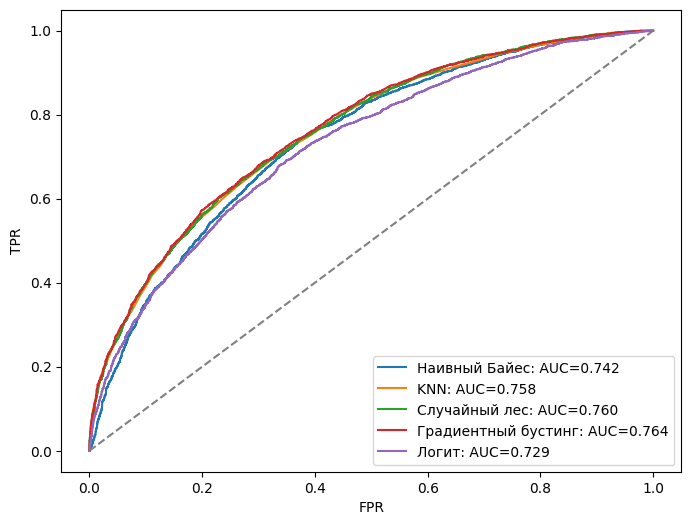
\includegraphics[keepaspectratio,alt={ROC-кривые и AUC пяти классификаторов}]{report_assets/block3_cell_44_output_0.png}}
\caption{ROC-кривые и AUC пяти классификаторов}
\end{figure}

{\def\LTcaptype{none} % do not increment counter
\begin{longtable}[]{@{}lr@{}}
\toprule\noalign{}
модель & AUC \\
\midrule\noalign{}
\endhead
\bottomrule\noalign{}
\endlastfoot
Градиентный бустинг & 0.764 \\
Случайный лес & 0.760 \\
KNN & 0.758 \\
Наивный Байес & 0.742 \\
Логит & 0.729 \\
\end{longtable}
}

    Чем выше ROC-кривая и чем больше AUC, тем лучше модель отделяет клиентов
с подпиской от клиентов без подписки при разных порогах. В отличие от
accuracy, AUC оценивает не одно бинарное решение, а качество
ранжирования вероятностей.

По AUC на тестовой выборке лучший результат у градиентного бустинга
(\texttt{0.764}), далее идут случайный лес (\texttt{0.760}) и KNN
(\texttt{0.758}). Наивный Байес (\texttt{0.742}) и логит
(\texttt{0.729}) уступают. Это согласуется с содержательной DGP: в
данных есть нелинейные зависимости и взаимодействия, которые ансамбли
деревьев ловят лучше, чем линейная логистическая регрессия и наивный
Байес с сильной предпосылкой условной независимости.

    Сохраним AUC для трех базовых моделей, чтобы итоговые таблицы и
дальнейшие блоки могли обращаться к тем же значениям.

    Повторный вывод таблицы фиксирует общий порядок пяти моделей по AUC на
тестовой выборке. В дальнейших итоговых сравнениях именно AUC
используется как основной критерий выбора лучшего и худшего
классификатора, потому что в прикладной задаче порог затем подбирается
отдельно по прибыли.

    \subsection{Задание 3.5}\label{ux437ux430ux434ux430ux43dux438ux435-3.5}

\begin{tasktext}
Для любой модели на ваш выбор постройте матрицу ошибок на тестовой
выборке при стандартном пороге классификации 0.50. Обсудите, какие
ошибки встречаются чаще и с чем это может быть связано.
\end{tasktext}

\subsubsection{Ответ}

Для каждой модели построим матрицу ошибок при стандартном пороге
классификации \(c=0.50\):

\begin{center}
\begin{adjustbox}{max width=\linewidth}
\(\displaystyle \hat D_i = \mathbb{1}\{\hat p_i \ge 0.50\}.\)
\end{adjustbox}
\end{center}

Матрица ошибок имеет вид

\begin{center}
\begin{adjustbox}{max width=\linewidth}
\(\displaystyle 
\begin{array}{c|cc}
 & \hat D=0 & \hat D=1 \\
\hline
D=0 & TN & FP \\
D=1 & FN & TP
\end{array}
\)
\end{adjustbox}
\end{center}

и показывает, какие типы ошибок делает модель.

    \textbf{Матрицы ошибок при стандартном пороге 0.50}

{\def\LTcaptype{none} % do not increment counter
\begin{longtable}[]{@{}lrrrr@{}}
\toprule\noalign{}
модель & TN & FP & FN & TP \\
\midrule\noalign{}
\endhead
\bottomrule\noalign{}
\endlastfoot
Наивный Байес & 2861 & 924 & 1550 & 2165 \\
KNN & 2710 & 1075 & 1291 & 2424 \\
Случайный лес & 2737 & 1048 & 1312 & 2403 \\
Градиентный бустинг & 2729 & 1056 & 1283 & 2432 \\
Логит & 2588 & 1197 & 1312 & 2403 \\
\end{longtable}
}

    Матрица ошибок показывает, какие ошибки встречаются чаще: ложные
срабатывания \texttt{FP} или пропуски подписчиков \texttt{FN}. Для
бизнес-задачи это важно, потому что разные ошибки могут иметь разную
стоимость.

При пороге \texttt{0.50} у всех моделей число \texttt{FP} и \texttt{FN}
достаточно велико, что ожидаемо при умеренной предсказательной силе
признаков. Например, градиентный бустинг дает \texttt{TP=2432},
\texttt{TN=2729}, \texttt{FP=1056}, \texttt{FN=1283}. Это означает, что
модель лучше случайного угадывания, но все еще часто путает клиентов
около границы решения. Поэтому дальнейший подбор порога по
бизнес-метрике действительно нужен: стандартный порог \texttt{0.50} не
обязан быть оптимальным для прибыли.

    \subsection{Задание 3.6}\label{ux437ux430ux434ux430ux43dux438ux435-3.6}

\begin{tasktext}
Для модели из предыдущего пункта рассмотрите не менее двух порогов,
отличных от 0.50, и рассчитайте для каждого из них ACC, Precision и
Recall. Результаты представьте в форме таблицы. Обсудите, как изменение
порога прогнозирования влияет на распределение ошибок прогнозов
различного типа. Уточните, какие из ошибок могут быть более
существенными исходя из контекста вашей экономической задачи.
Содержательно обоснуйте, какой из двух рассмотренных порогов может быть
предпочтительнее.
\end{tasktext}

\subsubsection{Ответ}

В задании требуется рассмотреть модель из предыдущего пункта. В пункте
3.5 матрицы ошибок были построены для всех моделей, поэтому для
аккуратного сопоставления ниже приводятся пороги для всех пяти
классификаторов. Это не меняет требование задания: для каждой модели,
включая выбранный в предыдущем пункте градиентный бустинг,
рассматриваются два порога, отличных от \texttt{0.50}, а именно
\texttt{0.30} и \texttt{0.70}. Дополнительно оставлен стандартный порог
\texttt{0.50} как база для сравнения.

При каждом пороге прогноз определяется правилом

\begin{center}
\begin{adjustbox}{max width=\linewidth}
\(\displaystyle \hat D_i(c) = \mathbb{1}\{\hat p_i \ge c\}.\)
\end{adjustbox}
\end{center}

Изменение \(c\) меняет соотношение между precision и recall: более
низкий порог делает модель менее строгой, а более высокий порог - более
строгой.

    \textbf{Качество моделей при разных порогах классификации}

{\def\LTcaptype{none} % do not increment counter
\begin{longtable}[]{@{}
  >{\raggedleft\arraybackslash}p{(\linewidth - 10\tabcolsep) * \real{0.1299}}
  >{\raggedright\arraybackslash}p{(\linewidth - 10\tabcolsep) * \real{0.2727}}
  >{\raggedleft\arraybackslash}p{(\linewidth - 10\tabcolsep) * \real{0.1688}}
  >{\raggedleft\arraybackslash}p{(\linewidth - 10\tabcolsep) * \real{0.1299}}
  >{\raggedleft\arraybackslash}p{(\linewidth - 10\tabcolsep) * \real{0.1688}}
  >{\raggedleft\arraybackslash}p{(\linewidth - 10\tabcolsep) * \real{0.1299}}@{}}
\toprule\noalign{}
\begin{minipage}[b]{\linewidth}\raggedleft
модель
\end{minipage} & \begin{minipage}[b]{\linewidth}\raggedright
модель
\end{minipage} & \begin{minipage}[b]{\linewidth}\raggedleft
threshold
\end{minipage} & \begin{minipage}[b]{\linewidth}\raggedleft
ACC
\end{minipage} & \begin{minipage}[b]{\linewidth}\raggedleft
Precision
\end{minipage} & \begin{minipage}[b]{\linewidth}\raggedleft
Recall
\end{minipage} \\
\midrule\noalign{}
\endhead
\bottomrule\noalign{}
\endlastfoot
0 & Наивный Байес & 0.30 & 0.623 & 0.575 & 0.917 \\
1 & Наивный Байес & 0.50 & 0.670 & 0.701 & 0.583 \\
2 & Наивный Байес & 0.70 & 0.593 & 0.795 & 0.240 \\
3 & KNN & 0.30 & 0.635 & 0.585 & 0.908 \\
4 & KNN & 0.50 & 0.685 & 0.693 & 0.652 \\
5 & KNN & 0.70 & 0.637 & 0.807 & 0.353 \\
6 & Случайный лес & 0.30 & 0.628 & 0.577 & 0.931 \\
7 & Случайный лес & 0.50 & 0.685 & 0.696 & 0.647 \\
8 & Случайный лес & 0.70 & 0.624 & 0.830 & 0.302 \\
9 & Градиентный бустинг & 0.30 & 0.637 & 0.585 & 0.919 \\
10 & Градиентный бустинг & 0.50 & 0.688 & 0.697 & 0.655 \\
11 & Градиентный бустинг & 0.70 & 0.627 & 0.828 & 0.312 \\
12 & Логит & 0.30 & 0.600 & 0.558 & 0.918 \\
13 & Логит & 0.50 & 0.665 & 0.667 & 0.647 \\
14 & Логит & 0.70 & 0.607 & 0.804 & 0.273 \\
\end{longtable}
}

    При снижении порога модель чаще прогнозирует подписку, поэтому recall
обычно растет, а precision может снижаться. При повышении порога прогноз
становится осторожнее: precision растет, но часть настоящих подписчиков
чаще попадает в пропуски.

В таблице это видно для всех моделей: при пороге \texttt{0.30} recall
примерно около \texttt{0.91-0.93}, то есть модель находит почти всех
подписчиков, но precision ниже. При пороге \texttt{0.70} precision
возрастает примерно до \texttt{0.80-0.83}, но recall падает до
\texttt{0.24-0.35}.

Если задача состоит в том, чтобы найти как можно больше клиентов,
которые действительно оформят подписку самостоятельно, предпочтительнее
низкий порог \texttt{0.30}, потому что он уменьшает число пропущенных
подписчиков (\texttt{FN}). Если важнее не ошибаться в положительных
прогнозах, предпочтительнее высокий порог \texttt{0.70}, потому что он
уменьшает число ложноположительных прогнозов (\texttt{FP}). В нашей
экономической постановке особенно существенны \texttt{FN}: такой клиент
фактически склонен к подписке, но модель относит его к неподписчикам, и
в следующей бизнес-логике ему могут зря отправить промокод. Поэтому из
двух нестандартных порогов более осторожным для бюджета является
\texttt{0.70}, а для общей статистической точности компромиссным
вариантом остается стандартный порог \texttt{0.50}, потому что при нем
accuracy обычно выше, чем при крайних порогах.

    \subsection{Задание 3.7}\label{ux437ux430ux434ux430ux43dux438ux435-3.7}

\begin{tasktext}
Обсудите прикладную задачу, для решения которой может использоваться
ваша классификационная модель. Опишите конкретного экономического агента
(заказчика), который может быть заинтересован в использовании ваших
прогнозов. Укажите, какие действия целесообразно предпринимать заказчику
в зависимости от того, является ваш прогноз положительным или
отрицательным. Исходя из этих действий и содержательных соображений
предположите цены различных видов прогнозов. Руководствуясь критерием
максимизации прибыли на обучающей выборке, подберите оптимальный порог
прогнозирования для каждого из методов и сравните прибыли на тестовой
выборке при соответствующих порогах. Результат представьте в форме
таблицы, в которой должны быть указаны прибыли на тестовой выборке.
Проинтерпретируйте полученный результат, в частности, объяснив, как
подобранное на данных оптимальное значение порога соотносится с
экономической интуицией.
\end{tasktext}

\subsubsection{Ответ}

Рассмотрим прикладную задачу: сервис доставки использует прогноз, чтобы
решать, кому отправлять промокод на бесплатный пробный период
премиум-подписки. Важно зафиксировать направление управленческого
действия. Положительный класс в классификации означает
\texttt{premium\_subscription\ =\ 1}, то есть клиент с высокой
вероятностью оформит подписку сам. Поэтому воздействовать промокодом
логичнее не на положительный прогноз, а на отрицательный: действие
применяется к клиентам, для которых модель прогнозирует отсутствие
подписки.

Для заданного порога \(c\) прибыль модели записывается как

\begin{center}
\begin{adjustbox}{max width=\linewidth}
\(\displaystyle Profit(c) = p_{TP}TP(c) + p_{TN}TN(c) + p_{FP}FP(c) + p_{FN}FN(c),\)
\end{adjustbox}
\end{center}

где \(p_{TP}, p_{TN}, p_{FP}, p_{FN}\) - цены соответствующих исходов.
Оптимальный порог выбирается на обучающей выборке:

\begin{center}
\begin{adjustbox}{max width=\linewidth}
\(\displaystyle c^* = \arg\max_c Profit_{train}(c).\)
\end{adjustbox}
\end{center}

    Зададим цены исходов относительно сценария, в котором компания ничего не
делает.

    \textbf{Цены ошибок и верных прогнозов для линейной прибыли}

TP 0 TN 100 FP 0 FN -500 dtype: int64

    Положительная прибыль у \texttt{TN} означает полезное действие для
клиента, который без промокода не оформил бы подписку: модель верно
относит его к классу 0, и компания может попытаться подтолкнуть его
промокодом. Отрицательная прибыль у \texttt{FN} отражает лишнюю
стоимость промокода для клиента, который на самом деле относится к
классу 1 и с высокой вероятностью подписался бы сам.

Важно, что здесь экономическая интерпретация отличается от стандартного
правила ``класс 1 = воздействовать''. В нашей постановке класс 1 - это
прогноз самостоятельной подписки, а промокод отправляется тем, для кого
прогноз равен 0. Поэтому \texttt{TN} - это удачно найденный клиент без
подписки, которому можно предложить промокод, а \texttt{FN} - подписчик,
которому промокод был отправлен зря. Такая запись не противоречит
confusion matrix: меняется не определение \texttt{TP/TN/FP/FN}, а
бизнес-действие, которое компания привязывает к отрицательному прогнозу.

    Запрограммируем функцию прибыли для произвольной модели и набора
порогов.

    Функция переводит вероятности в бинарные прогнозы при каждом пороге,
считает типы ошибок и умножает их на заданные цены. Это повторяет
семинарскую логику расчета прибыли: сначала строится прогноз при
конкретном \texttt{threshold}, затем через confusion matrix получаются
\texttt{TP}, \texttt{TN}, \texttt{FP}, \texttt{FN}, после чего считается
сумма цен прогнозов.

    Теперь выберем порог, максимизирующий прибыль на обучающей выборке, и
перенесем его на тестовую выборку. В коде перебираются уникальные
значения оцененных вероятностей на train:

\begin{center}
\begin{adjustbox}{max width=\linewidth}
\(\displaystyle c \in \{\hat p_i: i \in train\}.\)
\end{adjustbox}
\end{center}

Для каждого такого \(c\) считается \(Profit_{train}(c)\), после чего
выбранный \(c^*\) применяется к test.

    Такой порядок нужен, чтобы не подбирать порог по тестовой выборке. Test
используется только для финальной проверки прибыли.

В семинаре подчеркивалось, что порог \(c\) не обязан равняться
\texttt{0.50}: он должен отражать цены ошибок и верных прогнозов.
Поэтому мы сначала выбираем \(c^*\) на train, а затем оцениваем,
насколько выбранное правило переносится на test.

    Рассчитаем оптимальные пороги и тестовую прибыль для всех пяти
классификаторов.

    \textbf{Оптимальный порог и линейная прибыль на test}

{\def\LTcaptype{none} % do not increment counter
\begin{longtable}[]{@{}lrr@{}}
\toprule\noalign{}
модель & оптимальный порог & прибыль на тесте \\
\midrule\noalign{}
\endhead
\bottomrule\noalign{}
\endlastfoot
Случайный лес & 0.189 & 22500 \\
KNN & 0.173 & 18000 \\
Градиентный бустинг & 0.165 & 17700 \\
Наивный Байес & 0.169 & 15300 \\
Логит & 0.164 & 6400 \\
\end{longtable}
}

    Модель с наибольшей тестовой прибылью лучше подходит именно для этой
прикладной задачи. Оптимальный порог может быть ниже или выше 0.50,
потому что он отражает не статистическую симметрию ошибок, а заданные
экономические цены.

В полученной таблице оптимальные пороги для моделей находятся примерно в
диапазоне \texttt{0.16}-\texttt{0.19}, то есть заметно ниже стандартного
порога \texttt{0.50}. Это согласуется с экономической постановкой:
промокод отправляется тем, кому модель прогнозирует отсутствие подписки.
Низкий порог означает, что модель относит к классу \texttt{0} только
клиентов с достаточно малой оцененной вероятностью подписки. Так
компания избегает лишних промокодов для клиентов, которые с высокой
вероятностью подписались бы сами.

По тестовой прибыли лучшим оказывается случайный лес (\texttt{22500}).
Значит, хотя по AUC выше градиентный бустинг, при заданных ценах ошибок
и оптимальном пороге именно случайный лес дает более выгодное
управленческое правило. Это важный вывод: лучшая модель по
статистической метрике и лучшая модель по прибыли могут различаться.

    \subsubsection{Повышенная сложность к заданию
3.7}\label{ux43fux43eux432ux44bux448ux435ux43dux43dux430ux44f-ux441ux43bux43eux436ux43dux43eux441ux442ux44c-ux43a-ux437ux430ux434ux430ux43dux438ux44e-3.7}

Предложите, содержательно обоснуйте и примените собственную, отличную от
линейной функцию прибыли от прогнозов.

\subsubsection{Ответ}

Базовая функция прибыли линейно суммирует выгоды и издержки отдельных
прогнозов. Добавим более реалистичную бизнес-логику: если промокод
отправляется слишком большому числу клиентов, возникают дополнительные
организационные издержки, нагрузка на маркетинговый бюджет и риск
обесценивания акции.

В этой постановке промокод отправляется клиентам с прогнозом
\(\hat D_i=0\), потому что именно они считаются неподписчиками без
дополнительного стимула. Поэтому число клиентов, на которых направлено
воздействие, равно

\begin{center}
\begin{adjustbox}{max width=\linewidth}
\(\displaystyle Target(c)=TN(c)+FN(c).\)
\end{adjustbox}
\end{center}

Нелинейная прибыль задается как

\begin{center}
\begin{adjustbox}{max width=\linewidth}
\(\displaystyle Profit_{nonlinear}(c) = 100TN(c) - 500FN(c) - \gamma \cdot Target(c)^2.\)
\end{adjustbox}
\end{center}

Выберем \(\gamma = 0.0020\). Такой штраф почти не влияет при малом числе
промокодов, но быстро растет при массовой рассылке. Это отражает идею
ограниченного маркетингового бюджета: компания хочет помогать клиентам,
которые без промокода не подписались бы, но не хочет делать слишком
широкую и дорогую акцию.

    Функции вручную считают элементы confusion matrix и добавляют
квадратичный штраф за масштаб воздействия. Готовые метрики качества для
расчета прибыли здесь не используются.

    Для каждой модели подберем порог по новой нелинейной прибыли на train.
Затем сравним его с порогом, найденным в базовой линейной постановке.

    \textbf{Сравнение линейной и нелинейной функции прибыли}

{\def\LTcaptype{none} % do not increment counter
\begin{longtable}[]{@{}
  >{\raggedright\arraybackslash}p{(\linewidth - 24\tabcolsep) * \real{0.0700}}
  >{\raggedleft\arraybackslash}p{(\linewidth - 24\tabcolsep) * \real{0.0900}}
  >{\raggedleft\arraybackslash}p{(\linewidth - 24\tabcolsep) * \real{0.1000}}
  >{\raggedleft\arraybackslash}p{(\linewidth - 24\tabcolsep) * \real{0.1567}}
  >{\raggedleft\arraybackslash}p{(\linewidth - 24\tabcolsep) * \real{0.1533}}
  >{\raggedleft\arraybackslash}p{(\linewidth - 24\tabcolsep) * \real{0.0867}}
  >{\raggedleft\arraybackslash}p{(\linewidth - 24\tabcolsep) * \real{0.0833}}
  >{\raggedleft\arraybackslash}p{(\linewidth - 24\tabcolsep) * \real{0.0967}}
  >{\raggedleft\arraybackslash}p{(\linewidth - 24\tabcolsep) * \real{0.0833}}
  >{\raggedleft\arraybackslash}p{(\linewidth - 24\tabcolsep) * \real{0.0200}}
  >{\raggedleft\arraybackslash}p{(\linewidth - 24\tabcolsep) * \real{0.0200}}
  >{\raggedleft\arraybackslash}p{(\linewidth - 24\tabcolsep) * \real{0.0200}}
  >{\raggedleft\arraybackslash}p{(\linewidth - 24\tabcolsep) * \real{0.0200}}@{}}
\toprule\noalign{}
\begin{minipage}[b]{\linewidth}\raggedright
модель
\end{minipage} & \begin{minipage}[b]{\linewidth}\raggedleft
threshold linear profit
\end{minipage} & \begin{minipage}[b]{\linewidth}\raggedleft
threshold nonlinear profit
\end{minipage} & \begin{minipage}[b]{\linewidth}\raggedleft
train nonlinear profit при linear threshold
\end{minipage} & \begin{minipage}[b]{\linewidth}\raggedleft
test nonlinear profit при linear threshold
\end{minipage} & \begin{minipage}[b]{\linewidth}\raggedleft
train nonlinear profit
\end{minipage} & \begin{minipage}[b]{\linewidth}\raggedleft
test nonlinear profit
\end{minipage} & \begin{minipage}[b]{\linewidth}\raggedleft
positive predictions test
\end{minipage} & \begin{minipage}[b]{\linewidth}\raggedleft
targeted clients test
\end{minipage} & \begin{minipage}[b]{\linewidth}\raggedleft
TP
\end{minipage} & \begin{minipage}[b]{\linewidth}\raggedleft
FP
\end{minipage} & \begin{minipage}[b]{\linewidth}\raggedleft
FN
\end{minipage} & \begin{minipage}[b]{\linewidth}\raggedleft
TN
\end{minipage} \\
\midrule\noalign{}
\endhead
\bottomrule\noalign{}
\endlastfoot
Случайный лес & 0.189 & 0.19 & 75669.40 & 21829.50 & 74344.80 & 21522.60
& 6918 & 582 & 3655 & 3263 & 60 & 522 \\
Градиентный бустинг & 0.165 & 0.17 & 65760.80 & 17148.80 & 63472.30 &
19959.30 & 6934 & 566 & 3655 & 3279 & 60 & 506 \\
KNN & 0.173 & 0.17 & 68195 & 17562 & 68195 & 17562 & 7032 & 468 & 3667 &
3365 & 48 & 420 \\
Наивный Байес & 0.169 & 0.17 & 39367.80 & 15018.80 & 38520 & 15215.70 &
7123 & 377 & 3678 & 3445 & 37 & 340 \\
Логит & 0.164 & 0.17 & 19281.30 & 6256.35 & 17973.90 & 5015.17 & 7196 &
304 & 3673 & 3523 & 42 & 262 \\
\end{longtable}
}

    Таблица показывает, как меняется стратегия после добавления нелинейного
штрафа. В отличие от линейной прибыли, новая функция отдельно учитывает
масштаб промоакции через \texttt{targeted\ clients\ test}: если порог
приводит к слишком широкой рассылке, квадратичный штраф снижает итоговую
прибыль.

У случайного леса линейный и нелинейный пороги почти совпадают
(\texttt{0.189} и \texttt{0.19}), поэтому стратегия устойчива к
добавлению штрафа. У градиентного бустинга порог также остается близким
(\texttt{0.165} и \texttt{0.17}). При этом по нелинейной прибыли
случайный лес снова оказывается лучшим (\texttt{21522.55}). Это
означает, что он лучше балансирует между выгодой от таргетирования и
затратами на слишком широкое воздействие.

    \textbf{Лучшая модель по нелинейной прибыли}

Лучшая модель по нелинейной прибыли: Случайный лес Оптимальный threshold
для лучшей модели: 0.19 Максимальная test nonlinear profit: 21522.55

    По нелинейной прибыли лучшей считается модель с максимальным
\texttt{test\ nonlinear\ profit}. Если оптимальный нелинейный порог
отличается от линейного, это означает, что учет ограниченного
маркетингового бюджета меняет управленческую стратегию: модель выбирает
не просто максимум ожидаемой выгоды по отдельным клиентам, а баланс
между выгодой и масштабом воздействия.

В нашем случае нелинейная прибыль не переворачивает общий бизнес-вывод:
лучшим остается случайный лес. Но сама таблица становится богаче: она
показывает не только прибыль, но и число клиентов, на которых
направляется воздействие (\texttt{targeted\ clients\ test}), а также
\texttt{TP}, \texttt{FP}, \texttt{FN}, \texttt{TN}. Это делает решение
более интерпретируемым для заказчика.

    \subsection{Задание 3.8}\label{ux437ux430ux434ux430ux43dux438ux435-3.8}

\begin{tasktext}
Опишите предполагаемые связи между переменными в форме ориентированного
ациклического графа (DAG). Обучите структуру Байесовской сети на
обучающей выборке и сравните точность прогнозов вашего и обученного DAG
на тестовой выборке.
\end{tasktext}

\subsubsection{Ответ}

Зададим содержательный DAG между наблюдаемыми признаками и переменной
\texttt{premium\_subscription}, затем сравним его прогнозы с DAG,
структура которого обучена по данным.

В Байесовской сети совместное распределение переменных раскладывается по
графу:

\begin{center}
\begin{adjustbox}{max width=\linewidth}
\(\displaystyle P(V_1, \ldots, V_m) = \prod_{j=1}^{m} P(V_j \mid Pa(V_j)),\)
\end{adjustbox}
\end{center}

где \(Pa(V_j)\) - родители узла \(V_j\) в DAG. Для прогноза подписки
используется условное распределение

\begin{center}
\begin{adjustbox}{max width=\linewidth}
\(\displaystyle P(D_i = 1 \mid X_i).\)
\end{adjustbox}
\end{center}

    Сначала построим пользовательский DAG на основе экономической логики
задачи.

    \textbf{Пользовательский DAG Байесовской сети}

\begin{figure}
\centering
\pandocbounded{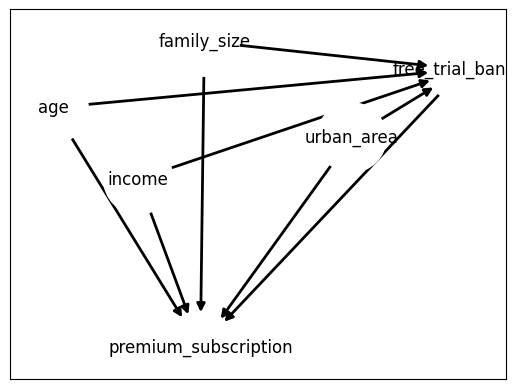
\includegraphics[keepaspectratio,alt={Пользовательский DAG Байесовской сети}]{report_assets/block3_cell_78_output_0.png}}
\caption{Пользовательский DAG Байесовской сети}
\end{figure}

    На графе признаки влияют на вероятность подписки, а также на вероятность
показа баннера. Это соответствует содержательной истории таргетированной
маркетинговой акции.

DAG полезен тем, что явно фиксирует предположения о направлении связей.
В отличие от случайного леса или бустинга, Байесовская сеть не просто
строит черный ящик для прогноза, а задает факторизацию совместного
распределения через родительские узлы. Поэтому ее легче
интерпретировать, хотя она может уступать гибким ансамблям по качеству
прогноза.

    Для дискретной Байесовской сети разобьем непрерывные признаки на
интервалы. Вместо исходных \texttt{income} и \texttt{age} используются
дискретные переменные

\begin{center}
\begin{adjustbox}{max width=\linewidth}
\(\displaystyle income\_bin_i \in \{0,1,2\}, \qquad age\_bin_i \in \{0,1,2\}.\)
\end{adjustbox}
\end{center}

Границы бинов оцениваются только на train и затем применяются к test.

    Такой биннинг не использует тестовую выборку при выборе границ, поэтому
прогноз Байесовской сети проверяется на честном test.

Биннинг нужен потому, что используемая дискретная Байесовская сеть
оценивает таблицы условных вероятностей для конечного числа состояний.
Для \texttt{income} и \texttt{age} строятся три группы, а
бинарные/дискретные признаки уже имеют конечное число значений.

    Оценим параметры пользовательского DAG на обучающей выборке. При
фиксированной структуре графа оцениваются условные вероятности вида

\begin{center}
\begin{adjustbox}{max width=\linewidth}
\(\displaystyle \widehat{P}(V_j = v \mid Pa(V_j) = pa),\)
\end{adjustbox}
\end{center}

то есть таблицы условных вероятностей для каждого узла.

    В этом блоке структура задана вручную, а условные вероятности в узлах
оцениваются по обучающим данным. Иными словами, мы фиксируем
экономическую структуру DAG, а затем по train оцениваем таблицы вида
\(P(V_j \mid Pa(V_j))\). Это отделяет содержательную часть модели от
статистической оценки параметров.

    Получим прогноз пользовательского DAG на тестовой выборке.

    Полученная accuracy показывает, насколько хорошо содержательно заданный
DAG прогнозирует подписку на тестовой выборке. Пользовательский DAG дает
test accuracy около \texttt{0.677}, что сопоставимо с более простыми
классификаторами, но ниже лучших ансамблей деревьев. Это нормальный
результат: ручная структура более интерпретируема, но менее гибка.

    Теперь обучим структуру DAG автоматически на train.

    Автоматически обученная структура отражает зависимости, которые алгоритм
находит в данных по выбранному критерию качества структуры. В отличие от
пользовательского DAG, здесь направления и наличие ребер выбираются
алгоритмом, поэтому результат может лучше подстроиться под данные, но
стать менее прозрачным содержательно.

    Сравним точность пользовательского и обученного DAG на одной и той же
тестовой выборке.

    Сравнение показывает, дает ли автоматическое обучение структуры выигрыш
относительно содержательного DAG. В текущих результатах accuracy
пользовательского DAG и обученного DAG почти совпадают: около
\texttt{0.677}. Это означает, что ручная структура уже хорошо отражает
основные зависимости в данных, а автоматическое обучение структуры не
дает заметного прироста качества по accuracy.

В базовом пункте задания требуется сравнить точность прогнозов
пользовательского и обученного DAG на тестовой выборке, поэтому здесь
Байесовские сети сопоставляются именно по \texttt{ACC\ test}. Дальше в
повышенной сложности мы дополнительно сравниваем их по ROC/AUC, то есть
по качеству ранжирования вероятностей.

    \subsubsection{Повышенная сложность к заданию
3.8}\label{ux43fux43eux432ux44bux448ux435ux43dux43dux430ux44f-ux441ux43bux43eux436ux43dux43eux441ux442ux44c-ux43a-ux437ux430ux434ux430ux43dux438ux44e-3.8}

Постройте ROC-кривую для Байесовской сети и сравните ее AUC с теми, что
были получены для иных методов.

\subsubsection{Ответ}

Для ROC-кривой нужны не только бинарные классы \(0/1\), а оцененные
вероятности положительного класса:

\begin{center}
\begin{adjustbox}{max width=\linewidth}
\(\displaystyle \widehat P(D_i = 1 \mid X_i).\)
\end{adjustbox}
\end{center}

\texttt{bnlearn.predict} возвращает предсказанный класс и вероятность
этого предсказанного класса. Поэтому вероятность положительного класса
восстанавливается так: если Байесовская сеть предсказала \texttt{1},
берем \texttt{p}; если предсказала \texttt{0}, берем \texttt{1-p}. Это
дает сопоставимый с другими моделями скоринг для построения ROC и
расчета AUC.

    Теперь построим ROC-кривые для пользовательского и обученного DAG на
тестовой выборке.

    \textbf{ROC-кривая и AUC Байесовской сети}

\begin{figure}
\centering
\pandocbounded{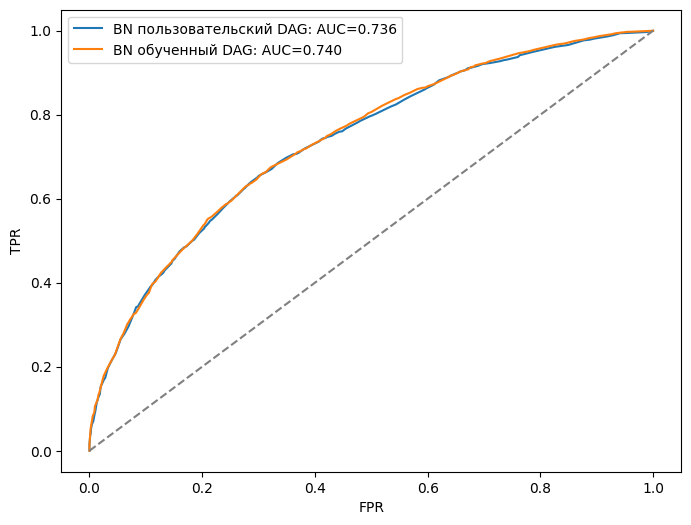
\includegraphics[keepaspectratio,alt={ROC-кривая и AUC Байесовской сети}]{report_assets/block3_cell_98_output_0.png}}
\caption{ROC-кривая и AUC Байесовской сети}
\end{figure}

{\def\LTcaptype{none} % do not increment counter
\begin{longtable}[]{@{}lr@{}}
\toprule\noalign{}
модель & AUC \\
\midrule\noalign{}
\endhead
\bottomrule\noalign{}
\endlastfoot
Байесовская сеть: пользовательский DAG & 0.736 \\
Байесовская сеть: обученный DAG & 0.740 \\
\end{longtable}
}

    Для сравнения добавим Байесовскую сеть в общую таблицу AUC вместе с
пятью классификаторами из предыдущих пунктов.

    \textbf{Сравнение AUC Байесовской сети с другими классификаторами}

{\def\LTcaptype{none} % do not increment counter
\begin{longtable}[]{@{}lr@{}}
\toprule\noalign{}
модель & AUC \\
\midrule\noalign{}
\endhead
\bottomrule\noalign{}
\endlastfoot
Градиентный бустинг & 0.764 \\
Случайный лес & 0.760 \\
KNN & 0.758 \\
Наивный Байес & 0.742 \\
Байесовская сеть: обученный DAG & 0.740 \\
Байесовская сеть: пользовательский DAG & 0.736 \\
Логит & 0.729 \\
\end{longtable}
}

    Таблица сравнивает качество ранжирования по вероятностям. Если AUC
Байесовской сети ниже AUC лучших ансамблевых моделей, это означает, что
сеть хуже ранжирует клиентов по вероятности подписки.

В нашем случае обученный DAG имеет AUC около \texttt{0.741},
пользовательский DAG - около \texttt{0.736}. Это немного ниже
градиентного бустинга (\texttt{0.764}), случайного леса (\texttt{0.760})
и KNN (\texttt{0.758}), но выше логистической регрессии
(\texttt{0.729}). Возможная причина результата: Байесовская сеть более
интерпретируема и явно опирается на структуру зависимостей, тогда как
случайный лес и градиентный бустинг лучше ловят сложные нелинейные
пороги и взаимодействия между признаками.

    \textbf{Сравнение лучшей базовой модели и Байесовской сети по AUC}

Лучшая базовая модель по AUC: Градиентный бустинг 0.764 Лучшая
Байесовская сеть по AUC: Байесовская сеть: обученный DAG 0.740 Разница
AUC лучшей базовой модели и лучшей BN: 0.024

    ROC/AUC показывает именно качество ранжирования вероятностей, а не
качество одного фиксированного порога. Поэтому Байесовская сеть может
иметь accuracy, близкую к другим моделям при пороге/правиле
классификации, но уступать по AUC, если ее вероятности хуже
упорядочивают клиентов от менее склонных к подписке к более склонным.

Содержательно это означает, что BN можно использовать как
интерпретируемую вероятностную модель, но если главная цель -
максимально точное ранжирование клиентов для последующего выбора порога,
то ансамблевые методы остаются предпочтительнее.

    \subsection{Задание 3.9}\label{ux437ux430ux434ux430ux43dux438ux435-3.9}

\begin{tasktext}
На основании проделанного анализа выберите лучший и худший из обученных
классификаторов. Обсудите полученный результат.

Примечание: необходимо самостоятельно сформулировать разумный критерий,
в соответствии с которым будут определяться лучшая и худшая модели.
\end{tasktext}

\subsubsection{Ответ}

Выберем лучший и худший классификатор по AUC на тестовой выборке.
Критерий выбора:

\begin{center}
\begin{adjustbox}{max width=\linewidth}
\(\displaystyle m_{best} = \arg\max_m AUC_m,\)
\end{adjustbox}
\end{center}

\begin{center}
\begin{adjustbox}{max width=\linewidth}
\(\displaystyle m_{worst} = \arg\min_m AUC_m.\)
\end{adjustbox}
\end{center}

Этот критерий подходит здесь, потому что дальше порог можно выбирать
отдельно под экономическую задачу.

    \textbf{Итоговая таблица качества пяти классификаторов}

{\def\LTcaptype{none} % do not increment counter
\begin{longtable}[]{@{}lrrr@{}}
\toprule\noalign{}
модель & test-ACC & AUC & CV-ACC \\
\midrule\noalign{}
\endhead
\bottomrule\noalign{}
\endlastfoot
Градиентный бустинг & 0.688 & 0.764 & 0.696 \\
Случайный лес & 0.685 & 0.760 & 0.694 \\
KNN & 0.685 & 0.758 & 0.693 \\
Наивный Байес & 0.670 & 0.742 & 0.674 \\
Логит & 0.665 & 0.729 & 0.669 \\
\end{longtable}
}

    Итоговая таблица объединяет test accuracy, AUC и CV accuracy для моделей
после тюнинга по accuracy.

    \textbf{Лучшие и худшие классификаторы по AUC}

Три лучших классификатора по AUC: test-ACC AUC CV-ACC модель\\
Градиентный бустинг 0.688 0.764 0.696 Случайный лес 0.685 0.760 0.694
KNN 0.685 0.758 0.693

Лучшая модель: Градиентный бустинг Худшая модель: Логит

    Лучшая модель имеет максимальный AUC на тестовой выборке, то есть лучше
всего ранжирует клиентов по вероятности подписки. Худшая модель имеет
минимальный AUC среди рассмотренных классификаторов.

По итоговой таблице лучший классификатор из методов курса - градиентный
бустинг (\texttt{AUC\ =\ 0.764}), худший - логистическая регрессия
(\texttt{AUC\ =\ 0.729}). Разница объясняется тем, что градиентный
бустинг строит последовательный ансамбль деревьев и способен ловить
нелинейности, а логит задает линейную зависимость логарифма шансов от
признаков. При этом по бизнес-прибыли лучший метод может отличаться от
лучшего по AUC, поэтому итоговый выбор модели зависит от цели:
ранжирование вероятностей или максимизация прибыли.

    \subsection{Задание 3.10. Повышенная
сложность}\label{ux437ux430ux434ux430ux43dux438ux435-3.10.-ux43fux43eux432ux44bux448ux435ux43dux43dux430ux44f-ux441ux43bux43eux436ux43dux43eux441ux442ux44c}

\begin{tasktext}
Включите в анализ дополнительный метод классификации, не
рассматривавшийся в курсе и не представленный в библиотеке scikit-learn.
Опишите данный метод (принцип работы, преимущества и недостатки) и
осуществите тюнинг гиперпараметров. Сопоставьте его точность на тестовой
выборке с точностью лучшего из обученных вами ранее методов. Добавление
обычной регуляризации к классическим методам не считается отдельным
методом.
\end{tasktext}

\subsubsection{Ответ}

Добавим дополнительный метод классификации, который не рассматривался в
курсе и не является моделью из \texttt{scikit-learn}:
\texttt{CatBoostClassifier} из библиотеки \texttt{catboost}.

CatBoost - это градиентный бустинг над решающими деревьями. Его важные
особенности: ordered boosting, снижающий смещение при обучении, и
удобная работа с категориальными признаками без ручного one-hot
encoding. В этой задаче категориальными считаем \texttt{urban\_area},
\texttt{family\_size} и \texttt{free\_trial\_banner}; непрерывные
\texttt{income} и \texttt{age} передаются как числовые признаки.

Преимущества CatBoost: он хорошо ловит нелинейности и взаимодействия
признаков, часто дает сильное качество без сложной предобработки
категорий. Недостатки: модель менее интерпретируема, имеет больше
гиперпараметров и может переобучаться при слишком большой глубине или
числе итераций.

    Зададим компактную сетку гиперпараметров, чтобы тюнинг был
воспроизводимым и не слишком тяжелым. Как и в семинарском
\texttt{GridSearchCV}, перебираются заранее заданные комбинации
параметров. Для CatBoost важны число итераций бустинга, глубина
деревьев, скорость обучения и L2-регуляризация листьев.

    Подберем гиперпараметры CatBoost по accuracy на кросс-валидации, чтобы
сравнение было согласовано с основной таблицей моделей. Категориальные
признаки передаются через \texttt{cat\_features}, поэтому CatBoost сам
строит внутренние кодировки категорий и не требует ручного one-hot
encoding.

    \textbf{Итоговое качество CatBoostClassifier}

{\def\LTcaptype{none} % do not increment counter
\begin{longtable}[]{@{}
  >{\raggedright\arraybackslash}p{(\linewidth - 22\tabcolsep) * \real{0.0407}}
  >{\raggedright\arraybackslash}p{(\linewidth - 22\tabcolsep) * \real{0.2073}}
  >{\raggedleft\arraybackslash}p{(\linewidth - 22\tabcolsep) * \real{0.0528}}
  >{\raggedleft\arraybackslash}p{(\linewidth - 22\tabcolsep) * \real{0.0407}}
  >{\raggedleft\arraybackslash}p{(\linewidth - 22\tabcolsep) * \real{0.0488}}
  >{\raggedleft\arraybackslash}p{(\linewidth - 22\tabcolsep) * \real{0.0447}}
  >{\raggedleft\arraybackslash}p{(\linewidth - 22\tabcolsep) * \real{0.0488}}
  >{\raggedleft\arraybackslash}p{(\linewidth - 22\tabcolsep) * \real{0.0935}}
  >{\raggedleft\arraybackslash}p{(\linewidth - 22\tabcolsep) * \real{0.1098}}
  >{\raggedleft\arraybackslash}p{(\linewidth - 22\tabcolsep) * \real{0.0894}}
  >{\raggedleft\arraybackslash}p{(\linewidth - 22\tabcolsep) * \real{0.1220}}
  >{\raggedleft\arraybackslash}p{(\linewidth - 22\tabcolsep) * \real{0.1016}}@{}}
\toprule\noalign{}
\begin{minipage}[b]{\linewidth}\raggedright
модель
\end{minipage} & \begin{minipage}[b]{\linewidth}\raggedright
лучшие гиперпараметры
\end{minipage} & \begin{minipage}[b]{\linewidth}\raggedleft
train-ACC
\end{minipage} & \begin{minipage}[b]{\linewidth}\raggedleft
CV-ACC
\end{minipage} & \begin{minipage}[b]{\linewidth}\raggedleft
test-ACC
\end{minipage} & \begin{minipage}[b]{\linewidth}\raggedleft
test-F1
\end{minipage} & \begin{minipage}[b]{\linewidth}\raggedleft
test-AUC
\end{minipage} & \begin{minipage}[b]{\linewidth}\raggedleft
test custom utility
\end{minipage} & \begin{minipage}[b]{\linewidth}\raggedleft
linear profit threshold
\end{minipage} & \begin{minipage}[b]{\linewidth}\raggedleft
test linear profit
\end{minipage} & \begin{minipage}[b]{\linewidth}\raggedleft
nonlinear profit threshold
\end{minipage} & \begin{minipage}[b]{\linewidth}\raggedleft
test nonlinear profit
\end{minipage} \\
\midrule\noalign{}
\endhead
\bottomrule\noalign{}
\endlastfoot
CatBoost & \{`depth': 4, `iterations': 300, `l2\_leaf\_reg':\ldots{} &
0.704 & 0.698 & 0.686 & 0.670 & 0.763 & 0.340 & 0.174 & 21600 & 0.15 &
23087.90 \\
\end{longtable}
}

    Сравним CatBoost с лучшей моделью из методов курса по test-метрикам. В
качестве базовой лучшей модели берем классификатор с максимальным AUC из
пункта 3.9 - градиентный бустинг. Это честное сравнение дополнительного
внешнего метода с лучшим методом, который уже был обучен в основной
части блока.

    \textbf{Сравнение CatBoost с лучшей моделью из методов курса}

{\def\LTcaptype{none} % do not increment counter
\begin{longtable}[]{@{}
  >{\raggedright\arraybackslash}p{(\linewidth - 12\tabcolsep) * \real{0.1667}}
  >{\raggedleft\arraybackslash}p{(\linewidth - 12\tabcolsep) * \real{0.0952}}
  >{\raggedleft\arraybackslash}p{(\linewidth - 12\tabcolsep) * \real{0.0873}}
  >{\raggedleft\arraybackslash}p{(\linewidth - 12\tabcolsep) * \real{0.0952}}
  >{\raggedleft\arraybackslash}p{(\linewidth - 12\tabcolsep) * \real{0.1825}}
  >{\raggedleft\arraybackslash}p{(\linewidth - 12\tabcolsep) * \real{0.1746}}
  >{\raggedleft\arraybackslash}p{(\linewidth - 12\tabcolsep) * \real{0.1984}}@{}}
\toprule\noalign{}
\begin{minipage}[b]{\linewidth}\raggedright
модель
\end{minipage} & \begin{minipage}[b]{\linewidth}\raggedleft
test-ACC
\end{minipage} & \begin{minipage}[b]{\linewidth}\raggedleft
test-F1
\end{minipage} & \begin{minipage}[b]{\linewidth}\raggedleft
test-AUC
\end{minipage} & \begin{minipage}[b]{\linewidth}\raggedleft
test custom utility
\end{minipage} & \begin{minipage}[b]{\linewidth}\raggedleft
test linear profit
\end{minipage} & \begin{minipage}[b]{\linewidth}\raggedleft
test nonlinear profit
\end{minipage} \\
\midrule\noalign{}
\endhead
\bottomrule\noalign{}
\endlastfoot
Градиентный бустинг & 0.688 & 0.675 & 0.764 & 0.358 & 17700 &
19959.30 \\
CatBoost & 0.686 & 0.670 & 0.763 & 0.340 & 21600 & 23087.90 \\
\end{longtable}
}

    Добавим CatBoost в общую таблицу AUC базовых классификаторов, чтобы
увидеть его место относительно моделей из курса. AUC здесь особенно
удобен: он сравнивает не один выбранный порог, а общее качество
вероятностного ранжирования клиентов.

    \textbf{Место CatBoost в общей таблице AUC}

{\def\LTcaptype{none} % do not increment counter
\begin{longtable}[]{@{}lr@{}}
\toprule\noalign{}
модель & AUC \\
\midrule\noalign{}
\endhead
\bottomrule\noalign{}
\endlastfoot
Градиентный бустинг & 0.764 \\
CatBoost & 0.763 \\
Случайный лес & 0.760 \\
KNN & 0.758 \\
Наивный Байес & 0.742 \\
Логит & 0.729 \\
\end{longtable}
}

    \textbf{Итог сравнения CatBoost с методами курса}

Лучшая модель из методов курса: Градиентный бустинг Лучшая модель после
добавления CatBoost: Градиентный бустинг Разница AUC CatBoost и лучшей
модели курса: -0.0007

    CatBoost почти догоняет лучшую модель из курса по AUC, но не улучшает
ее: у градиентного бустинга \texttt{AUC\ =\ 0.764}, у CatBoost
\texttt{AUC\ =\ 0.763}, разница около \texttt{-0.0007}. Это практически
паритет по качеству ранжирования, но формально лучшей моделью по AUC
остается градиентный бустинг.

При этом CatBoost дает более высокую нелинейную прибыль в сравнительной
таблице (\texttt{23087.93} против \texttt{19959.29} у градиентного
бустинга). Поэтому CatBoost полезен как сильный внешний benchmark: по
статистическому AUC он не превосходит лучший метод курса, но по
бизнес-критерию с нелинейным штрафом может быть предпочтительнее.
Итоговый выбор зависит от приоритета: если нужен простой и уже изученный
метод с лучшим AUC, выбираем градиентный бустинг; если важнее
бизнес-прибыль по нашей нелинейной функции, CatBoost выглядит
привлекательнее, хотя он менее интерпретируем и требует внешней
библиотеки.

    \subsection{Задание
3.11}\label{ux437ux430ux434ux430ux43dux438ux435-3.11}

\begin{tasktext}
В случае необходимости проведите дополнительный анализ.
\end{tasktext}

\subsubsection{Ответ}

Проведем дополнительные проверки, которые помогают интерпретировать
качество классификаторов и убедиться, что результаты не сводятся к
простому дисбалансу классов или одному признаку.

Доля единиц в выборке считается как

\begin{center}
\begin{adjustbox}{max width=\linewidth}
\(\displaystyle \bar D = \frac{1}{n}\sum_{i=1}^{n} D_i.\)
\end{adjustbox}
\end{center}

Попарное совпадение прогнозов двух моделей \(a\) и \(b\) считается как

\begin{center}
\begin{adjustbox}{max width=\linewidth}
\(\displaystyle Agreement(a,b) = \frac{1}{n}\sum_{i=1}^{n}\mathbb{1}\{\hat D_i^{a} = \hat D_i^{b}\}.\)
\end{adjustbox}
\end{center}

    Сначала посмотрим долю единиц в train и test.

    \textbf{Проверка долей классов в train и test}

{\def\LTcaptype{none} % do not increment counter
\begin{longtable}[]{@{}rlr@{}}
\toprule\noalign{}
модель & metric & value \\
\midrule\noalign{}
\endhead
\bottomrule\noalign{}
\endlastfoot
0 & train\_share\_ones & 0.494 \\
1 & test\_share\_ones & 0.495 \\
\end{longtable}
}

    Близкие доли единиц в train и test означают, что разбиение не создало
заметного сдвига по целевой переменной. В обеих выборках доля
подписчиков близка к \texttt{0.49-0.50}, поэтому различия в качестве
моделей нельзя объяснить тем, что в test случайно попал совсем другой
баланс классов.

    Сравним бинарные прогнозы моделей попарно.

    \textbf{Совпадение бинарных прогнозов между моделями}

{\def\LTcaptype{none} % do not increment counter
\begin{longtable}[]{@{}rlr@{}}
\toprule\noalign{}
модель & models & share\_equal \\
\midrule\noalign{}
\endhead
\bottomrule\noalign{}
\endlastfoot
8 & Случайный лес vs Логит & 0.846 \\
6 & KNN vs Логит & 0.851 \\
9 & Градиентный бустинг vs Логит & 0.853 \\
0 & Наивный Байес vs KNN & 0.858 \\
1 & Наивный Байес vs Случайный лес & 0.863 \\
2 & Наивный Байес vs Градиентный бустинг & 0.868 \\
3 & Наивный Байес vs Логит & 0.882 \\
4 & KNN vs Случайный лес & 0.927 \\
5 & KNN vs Градиентный бустинг & 0.932 \\
7 & Случайный лес vs Градиентный бустинг & 0.933 \\
\end{longtable}
}

    Если доля совпадающих прогнозов очень высока, модели фактически
принимают похожие решения. Если совпадение ниже, разные алгоритмы
по-разному используют структуру признаков.

В нашем случае совпадение прогнозов между некоторыми моделями находится
около \texttt{0.85-0.86}, а между KNN, случайным лесом и градиентным
бустингом выше \texttt{0.93}. Это означает, что сильные нелинейные
модели часто классифицируют клиентов похожим образом, но логит и наивный
Байес принимают более отличающиеся решения.

    Сравним предсказанные вероятности моделей. Для двух моделей \(a\) и
\(b\) считается корреляция между векторами вероятностей:

\begin{center}
\begin{adjustbox}{max width=\linewidth}
\(\displaystyle Corr(\hat p^a, \hat p^b) = Corr\left((\hat p_1^a, \ldots, \hat p_n^a), (\hat p_1^b, \ldots, \hat p_n^b)\right).\)
\end{adjustbox}
\end{center}

Эта проверка показывает, насколько похоже модели ранжируют клиентов.

    \textbf{Корреляция предсказанных вероятностей между моделями}

{\def\LTcaptype{none} % do not increment counter
\begin{longtable}[]{@{}rlr@{}}
\toprule\noalign{}
модель & models & corr \\
\midrule\noalign{}
\endhead
\bottomrule\noalign{}
\endlastfoot
6 & KNN vs Логит & 0.855 \\
8 & Случайный лес vs Логит & 0.856 \\
0 & Наивный Байес vs KNN & 0.860 \\
9 & Градиентный бустинг vs Логит & 0.863 \\
1 & Наивный Байес vs Случайный лес & 0.875 \\
2 & Наивный Байес vs Градиентный бустинг & 0.879 \\
3 & Наивный Байес vs Логит & 0.892 \\
4 & KNN vs Случайный лес & 0.959 \\
5 & KNN vs Градиентный бустинг & 0.962 \\
7 & Случайный лес vs Градиентный бустинг & 0.979 \\
\end{longtable}
}

    Корреляция вероятностей показывает, насколько похоже модели ранжируют
клиентов, даже если бинарные прогнозы при пороге 0.50 частично
совпадают.

Высокая корреляция вероятностей между случайным лесом и градиентным
бустингом означает, что эти модели не только часто дают одинаковые
классы, но и похожим образом упорядочивают клиентов по вероятности
подписки. Более низкая корреляция с логитом показывает, что линейная
модель видит структуру риска иначе.

    Для случайного леса и градиентного бустинга посмотрим важность
признаков.

    \textbf{Важность признаков в случайном лесе и градиентном бустинге}

{\def\LTcaptype{none} % do not increment counter
\begin{longtable}[]{@{}lrr@{}}
\toprule\noalign{}
модель & rf\_importance & gb\_importance \\
\midrule\noalign{}
\endhead
\bottomrule\noalign{}
\endlastfoot
income & 0.447 & 0.225 \\
age & 0.303 & 0.243 \\
family\_size & 0.119 & 0.185 \\
urban\_area & 0.077 & 0.195 \\
free\_trial\_banner & 0.055 & 0.152 \\
\end{longtable}
}

    Важности признаков показывают, какие переменные деревья чаще используют
для разделения клиентов. Это помогает понять, не доминирует ли один
признак над всей классификацией.

У случайного леса наибольшие важности получают \texttt{income} и
\texttt{age}, у градиентного бустинга вклад распределен более равномерно
между \texttt{income}, \texttt{age}, \texttt{urban\_area},
\texttt{family\_size} и \texttt{free\_trial\_banner}. Это хорошо: модель
не сводится только к инструменту \texttt{free\_trial\_banner}, а
использует несколько экономически осмысленных характеристик клиента.

    Проверим качество простого правила, которое использует только
\texttt{free\_trial\_banner}:

\begin{center}
\begin{adjustbox}{max width=\linewidth}
\(\displaystyle \hat D_i^{banner} = free\_trial\_banner_i.\)
\end{adjustbox}
\end{center}

Это базовое сравнение показывает, насколько далеко можно продвинуться
без обучения сложной модели.

    \textbf{Качество простого правила по баннеру}

{\def\LTcaptype{none} % do not increment counter
\begin{longtable}[]{@{}rlr@{}}
\toprule\noalign{}
модель & metric & value \\
\midrule\noalign{}
\endhead
\bottomrule\noalign{}
\endlastfoot
0 & ACC\_banner\_only & 0.609 \\
1 & Precision\_banner\_only & 0.654 \\
2 & Recall\_banner\_only & 0.445 \\
\end{longtable}
}

    Если лучшее качество моделей заметно выше качества простого правила по
баннеру, значит классификаторы используют не только инструмент, но и
остальные признаки.

Простое правило по \texttt{free\_trial\_banner} дает
\texttt{ACC\ =\ 0.609}, тогда как лучшая модель имеет
\texttt{ACC\ =\ 0.688}. Разрыв около \texttt{0.079} показывает, что
модели действительно извлекают дополнительную информацию из дохода,
возраста, города и размера семьи. Это важная диагностическая проверка:
классификация не должна превращаться в механическое повторение
инструмента.

    Соберем итоговую диагностическую таблицу по лучшей модели и простому
правилу.

    \textbf{Итоговая диагностическая проверка классификации}

{\def\LTcaptype{none} % do not increment counter
\begin{longtable}[]{@{}rlr@{}}
\toprule\noalign{}
модель & metric & value \\
\midrule\noalign{}
\endhead
\bottomrule\noalign{}
\endlastfoot
0 & ACC\_banner\_only & 0.609 \\
1 & ACC\_best\_model & 0.688 \\
2 & AUC\_best\_model & 0.764 \\
3 & ACC\_gap\_best\_minus\_banner & 0.079 \\
4 & min\_pairwise\_agreement & 0.846 \\
5 & max\_pairwise\_agreement & 0.933 \\
\end{longtable}
}

    Эта таблица резюмирует, насколько лучшая модель превосходит простое
правило и насколько похожи между собой прогнозы разных классификаторов.

Итоговая диагностика поддерживает основной вывод блока: данные не
являются тривиально предсказуемыми одним баннером, модели различаются
между собой, а лучший классификатор дает заметный, но не огромный
прирост качества. Поэтому дальнейший анализ эффектов воздействия должен
учитывать качество классификационной модели, но не переоценивать его:
прогноз воздействия остается умеренно точным, а не почти идеальным.

    \section{Блок 4.
Регрессия}\label{ux431ux43bux43eux43a-4.-ux440ux435ux433ux440ux435ux441ux441ux438ux44f}

\begin{tasktext}
\textbf{Текст задания.} В каждом из заданий, если не сказано иного,
необходимо использовать хотя бы 3 метода из следующих: случайный лес,
метод наименьших квадратов, метод ближайших соседей и градиентный
бустинг.
\end{tasktext}

\textbf{Ответ.} В этом разделе решается задача прогнозирования
непрерывной целевой переменной \texttt{monthly\_spending}. Обозначим ее
как \(Y_i\), а вектор признаков клиента как \(X_i\). Цель регрессионной
модели - построить функцию \(\hat f(X_i)\), которая приближает условное
математическое ожидание:

\begin{center}
\begin{adjustbox}{max width=\linewidth}
\(\displaystyle \hat Y_i = \hat f(X_i) \approx E(Y_i \mid X_i).\)
\end{adjustbox}
\end{center}

В соответствии с условием задания переменная воздействия
\texttt{premium\_subscription} не включается в признаки. Это важно: если
бы мы добавили воздействие в регрессионную модель прогноза, модель
частично использовала бы информацию о treatment, что нарушило бы
постановку блока регрессии и могло бы повлиять на последующий анализ
эффектов воздействия.

Сначала подготавливаются данные, метрики и модели. Все модели обучаются
и сравниваются на одном и том же train/test split, чтобы результаты были
сопоставимы.

    \subsection{Задание 4.1}\label{ux437ux430ux434ux430ux43dux438ux435-4.1}

\begin{tasktext}
\textbf{Текст задания.} Отберите признаки, которые могут быть полезны
при прогнозировании целевой (зависимой) переменной. Не включайте в число
этих признаков переменную воздействия.
\end{tasktext}

\textbf{Ответ.} Целевая переменная:

\begin{center}
\begin{adjustbox}{max width=\linewidth}
\(\displaystyle Y_i = \text{monthly\_spending}_i.\)
\end{adjustbox}
\end{center}

Матрица признаков:

\begin{center}
\begin{adjustbox}{max width=\linewidth}
\(\displaystyle X_i = (\text{income}_i, \text{age}_i, \text{urban\_area}_i, \text{family\_size}_i, \text{free\_trial\_banner}_i).\)
\end{adjustbox}
\end{center}

Переменная воздействия \(D_i = \text{premium\_subscription}_i\) не
входит в \(X_i\).

{\def\LTcaptype{none} % do not increment counter
\begin{longtable}[]{@{}ll@{}}
\toprule\noalign{}
переменная & роль \\
\midrule\noalign{}
\endhead
\bottomrule\noalign{}
\endlastfoot
\texttt{monthly\_spending} & целевая переменная \\
\texttt{income} & признак \\
\texttt{age} & признак \\
\texttt{urban\_area} & признак \\
\texttt{family\_size} & признак \\
\texttt{free\_trial\_banner} & признак \\
\end{longtable}
}

В качестве признаков используются доход, возраст, тип территории, размер
семьи и инструмент \texttt{free\_trial\_banner}. Такой набор
содержательно связан с месячными тратами: доход отражает
платежеспособность, возраст - жизненный цикл клиента, городская
территория - доступность сервиса, размер семьи - потенциальный объем
потребления. \texttt{free\_trial\_banner} не является переменной
воздействия; это инструментальная переменная из процесса генерации,
поэтому ее включение не нарушает прямой запрет на
\texttt{premium\_subscription}. Важно, что здесь
\texttt{free\_trial\_banner} используется только как прогнозный признак
в регрессионной задаче. В блоке оценки эффектов воздействия без
инструментальной переменной он не включается в causal controls, чтобы не
смешивать обычную корректировку по наблюдаемым признакам с
инструментальной вариацией.

Выборка разделена на обучающую и тестовую в пропорции 75/25:

{\def\LTcaptype{none} % do not increment counter
\begin{longtable}[]{@{}lr@{}}
\toprule\noalign{}
показатель & значение \\
\midrule\noalign{}
\endhead
\bottomrule\noalign{}
\endlastfoot
\texttt{n\_train} & 22500 \\
\texttt{n\_test} & 7500 \\
\texttt{test\_share} & 0.25 \\
\end{longtable}
}

Тестовая часть составляет 25\%, что соответствует требуемому интервалу
от 20\% до 30\%.

    \subsection{Задание 4.2}\label{ux437ux430ux434ux430ux43dux438ux435-4.2}

\begin{tasktext}
\textbf{Текст задания.} Для каждого метода оцените \texttt{RMSE} и
\texttt{MAPE}, используя произвольные значения гиперпараметров на
обучающей выборке, тестовой выборке и с помощью кросс-валидации. С
помощью кросс-валидации на обучающей выборке подберите оптимальные
значения гиперпараметров. В одной таблице укажите исходные и подобранные
значения гиперпараметров, а также \texttt{RMSE} и \texttt{MAPE},
рассчитанные на тестовой выборке и с помощью кросс-валидации до и после
тюнинга. Обсудите наличие или отсутствие признаков переобучения модели и
проинтерпретируйте полученные результаты.
\end{tasktext}

\textbf{Ответ.} Используются четыре метода: МНК, KNN, случайный лес и
градиентный бустинг, то есть больше минимально требуемых трех.

Метрики качества:

\begin{center}
\begin{adjustbox}{max width=\linewidth}
\(\displaystyle RMSE = \sqrt{\frac{1}{n}\sum_{i=1}^{n}(Y_i - \hat Y_i)^2},\)
\end{adjustbox}
\end{center}

\begin{center}
\begin{adjustbox}{max width=\linewidth}
\(\displaystyle MAPE = \frac{1}{n}\sum_{i=1}^{n}\left|\frac{Y_i - \hat Y_i}{Y_i}\right| \cdot 100\%.\)
\end{adjustbox}
\end{center}

\texttt{RMSE} измеряет типичный масштаб ошибки в единицах
\texttt{monthly\_spending}, поэтому используется как основной критерий
сравнения. \texttt{MAPE} показывает относительную ошибку и в таблицах
приведен в процентах: например, значение \texttt{94.661} означает
среднюю абсолютную процентную ошибку около \texttt{94.70\%}. В наших
данных есть очень малые значения \texttt{monthly\_spending}, поэтому
\texttt{MAPE} менее устойчива и используется только как дополнительная
метрика, а не как основной критерий выбора лучшей модели.

Кросс-валидационная оценка строится как среднее по фолдам:

\begin{center}
\begin{adjustbox}{max width=\linewidth}
\(\displaystyle CV = \frac{1}{K}\sum_{k=1}^{K}Q_k,\)
\end{adjustbox}
\end{center}

где \(Q_k\) - значение метрики на validation-части \(k\)-го фолда.

Методы устроены следующим образом. МНК оценивает линейную зависимость:

\begin{center}
\begin{adjustbox}{max width=\linewidth}
\(\displaystyle \hat Y_i = \hat\beta_0 + X_i'\hat\beta.\)
\end{adjustbox}
\end{center}

KNN-регрессия прогнозирует значение по ближайшим соседям; поскольку
расстояния зависят от масштаба признаков, используется стандартизация:

\begin{center}
\begin{adjustbox}{max width=\linewidth}
\(\displaystyle \tilde X_{ij} = \frac{X_{ij} - \bar X_j}{\hat\sigma_j}.\)
\end{adjustbox}
\end{center}

Случайный лес усредняет прогнозы деревьев:

\begin{center}
\begin{adjustbox}{max width=\linewidth}
\(\displaystyle \hat f_{RF}(x) = \frac{1}{B}\sum_{b=1}^{B}\hat f_b(x).\)
\end{adjustbox}
\end{center}

Градиентный бустинг строит ансамбль последовательно:

\begin{center}
\begin{adjustbox}{max width=\linewidth}
\(\displaystyle F_{m+1}(x) = F_m(x) + \gamma h_m(x),\)
\end{adjustbox}
\end{center}

где \(h_m(x)\) - очередное дерево, а \(\gamma\) соответствует
\texttt{learning\_rate}.

    \textbf{Исходные гиперпараметры моделей}

{\def\LTcaptype{none} % do not increment counter
\begin{longtable}[]{@{}
  >{\raggedright\arraybackslash}p{(\linewidth - 2\tabcolsep) * \real{0.5000}}
  >{\raggedright\arraybackslash}p{(\linewidth - 2\tabcolsep) * \real{0.5000}}@{}}
\toprule\noalign{}
\begin{minipage}[b]{\linewidth}\raggedright
модель
\end{minipage} & \begin{minipage}[b]{\linewidth}\raggedright
исходные гиперпараметры
\end{minipage} \\
\midrule\noalign{}
\endhead
\bottomrule\noalign{}
\endlastfoot
МНК & нет настраиваемых гиперпараметров \\
KNN & \texttt{n\_neighbors=25}, \texttt{weights=distance},
\texttt{StandardScaler} \\
Случайный лес & \texttt{max\_depth=10}, \texttt{max\_features=sqrt},
\texttt{n\_estimators=100} \\
Градиентный бустинг & \texttt{max\_depth=3},
\texttt{learning\_rate=0.07}, \texttt{n\_estimators=120} \\
\end{longtable}
}

\textbf{Качество до тюнинга}

{\def\LTcaptype{none} % do not increment counter
\begin{longtable}[]{@{}
  >{\raggedright\arraybackslash}p{(\linewidth - 12\tabcolsep) * \real{0.1111}}
  >{\raggedleft\arraybackslash}p{(\linewidth - 12\tabcolsep) * \real{0.1481}}
  >{\raggedleft\arraybackslash}p{(\linewidth - 12\tabcolsep) * \real{0.1481}}
  >{\raggedleft\arraybackslash}p{(\linewidth - 12\tabcolsep) * \real{0.1481}}
  >{\raggedleft\arraybackslash}p{(\linewidth - 12\tabcolsep) * \real{0.1481}}
  >{\raggedleft\arraybackslash}p{(\linewidth - 12\tabcolsep) * \real{0.1481}}
  >{\raggedleft\arraybackslash}p{(\linewidth - 12\tabcolsep) * \real{0.1481}}@{}}
\toprule\noalign{}
\begin{minipage}[b]{\linewidth}\raggedright
модель
\end{minipage} & \begin{minipage}[b]{\linewidth}\raggedleft
RMSE train
\end{minipage} & \begin{minipage}[b]{\linewidth}\raggedleft
MAPE train
\end{minipage} & \begin{minipage}[b]{\linewidth}\raggedleft
RMSE test
\end{minipage} & \begin{minipage}[b]{\linewidth}\raggedleft
MAPE test
\end{minipage} & \begin{minipage}[b]{\linewidth}\raggedleft
RMSE-CV
\end{minipage} & \begin{minipage}[b]{\linewidth}\raggedleft
MAPE-CV
\end{minipage} \\
\midrule\noalign{}
\endhead
\bottomrule\noalign{}
\endlastfoot
МНК & 5005.00 & 99.786 & 4983.14 & 97.411 & 5005.65 & 99.750 \\
KNN & 0.0000 & 0.0000 & 5004.85 & 99.046 & 5034.77 & 97.389 \\
Случайный лес & 4372.27 & 89.032 & 4749.34 & 99.927 & 4769.50 &
99.504 \\
Градиентный бустинг & 4672.24 & 95.501 & 4708.21 & 96.569 & 4729.15 &
96.689 \\
\end{longtable}
}

По исходным гиперпараметрам лучший результат по \texttt{RMSE\ test} дает
градиентный бустинг (\texttt{4708.21}), немного хуже работает случайный
лес (\texttt{4749.34}), затем идут МНК и KNN. Это согласуется с
устройством данных: зависимость \texttt{monthly\_spending} от признаков
нелинейная, поэтому ансамбли деревьев лучше аппроксимируют функцию
\(E(Y\mid X)\), чем линейная модель.

Особенно важен результат KNN: при \texttt{weights="distance"} на
обучающей выборке \texttt{RMSE\ =\ 0} и \texttt{MAPE\ =\ 0}. Это
означает, что модель фактически запоминает train-наблюдения. Но на test
и CV качество заметно хуже. Это классический признак переобучения.

    \textbf{Подбор гиперпараметров и итоговая таблица}

Подбор выполнялся по \texttt{RMSE} на кросс-валидации. Формально
выбиралась комбинация гиперпараметров:

\begin{center}
\begin{adjustbox}{max width=\linewidth}
\(\displaystyle \hat\lambda = \arg\min_{\lambda \in \Lambda} CV(\lambda).\)
\end{adjustbox}
\end{center}

{\def\LTcaptype{none} % do not increment counter
\begin{longtable}[]{@{}
  >{\raggedright\arraybackslash}p{(\linewidth - 28\tabcolsep) * \real{0.0526}}
  >{\raggedright\arraybackslash}p{(\linewidth - 28\tabcolsep) * \real{0.0526}}
  >{\raggedright\arraybackslash}p{(\linewidth - 28\tabcolsep) * \real{0.0526}}
  >{\raggedleft\arraybackslash}p{(\linewidth - 28\tabcolsep) * \real{0.0702}}
  >{\raggedleft\arraybackslash}p{(\linewidth - 28\tabcolsep) * \real{0.0702}}
  >{\raggedleft\arraybackslash}p{(\linewidth - 28\tabcolsep) * \real{0.0702}}
  >{\raggedleft\arraybackslash}p{(\linewidth - 28\tabcolsep) * \real{0.0702}}
  >{\raggedleft\arraybackslash}p{(\linewidth - 28\tabcolsep) * \real{0.0702}}
  >{\raggedleft\arraybackslash}p{(\linewidth - 28\tabcolsep) * \real{0.0702}}
  >{\raggedleft\arraybackslash}p{(\linewidth - 28\tabcolsep) * \real{0.0702}}
  >{\raggedleft\arraybackslash}p{(\linewidth - 28\tabcolsep) * \real{0.0702}}
  >{\raggedleft\arraybackslash}p{(\linewidth - 28\tabcolsep) * \real{0.0702}}
  >{\raggedleft\arraybackslash}p{(\linewidth - 28\tabcolsep) * \real{0.0702}}
  >{\raggedleft\arraybackslash}p{(\linewidth - 28\tabcolsep) * \real{0.0702}}
  >{\raggedleft\arraybackslash}p{(\linewidth - 28\tabcolsep) * \real{0.0702}}@{}}
\toprule\noalign{}
\begin{minipage}[b]{\linewidth}\raggedright
модель
\end{minipage} & \begin{minipage}[b]{\linewidth}\raggedright
исходные гиперпараметры
\end{minipage} & \begin{minipage}[b]{\linewidth}\raggedright
подобранные гиперпараметры
\end{minipage} & \begin{minipage}[b]{\linewidth}\raggedleft
RMSE train до
\end{minipage} & \begin{minipage}[b]{\linewidth}\raggedleft
RMSE train после
\end{minipage} & \begin{minipage}[b]{\linewidth}\raggedleft
MAPE train до
\end{minipage} & \begin{minipage}[b]{\linewidth}\raggedleft
MAPE train после
\end{minipage} & \begin{minipage}[b]{\linewidth}\raggedleft
RMSE test до
\end{minipage} & \begin{minipage}[b]{\linewidth}\raggedleft
RMSE test после
\end{minipage} & \begin{minipage}[b]{\linewidth}\raggedleft
MAPE test до
\end{minipage} & \begin{minipage}[b]{\linewidth}\raggedleft
MAPE test после
\end{minipage} & \begin{minipage}[b]{\linewidth}\raggedleft
RMSE-CV до
\end{minipage} & \begin{minipage}[b]{\linewidth}\raggedleft
RMSE-CV после
\end{minipage} & \begin{minipage}[b]{\linewidth}\raggedleft
MAPE-CV до
\end{minipage} & \begin{minipage}[b]{\linewidth}\raggedleft
MAPE-CV после
\end{minipage} \\
\midrule\noalign{}
\endhead
\bottomrule\noalign{}
\endlastfoot
Градиентный бустинг &
\texttt{max\_depth=3,\ learning\_rate=0.07,\ n\_estimators=120} &
\texttt{learning\_rate=0.10,\ max\_depth=3,\ n\_estimators=120} &
4672.24 & 4659.32 & 95.501 & 93.603 & 4708.21 & 4710.36 & 96.569 &
94.661 & 4729.15 & 4728.38 & 96.689 & 95.459 \\
Случайный лес &
\texttt{max\_depth=10,\ max\_features=sqrt,\ n\_estimators=100} &
\texttt{max\_depth=8,\ max\_features=sqrt,\ n\_estimators=120} & 4372.27
& 4605.23 & 89.032 & 100.15 & 4749.34 & 4732.91 & 99.927 & 104.13 &
4769.50 & 4760.95 & 99.504 & 104.10 \\
KNN & \texttt{n\_neighbors=25,\ weights=distance,\ StandardScaler} &
\texttt{n\_neighbors=45,\ weights=uniform} & 0.0000 & 4660.88 & 0.0000 &
99.555 & 5004.85 & 4760.31 & 99.046 & 103.21 & 5034.77 & 4771.43 &
97.389 & 102.99 \\
МНК & нет настраиваемых гиперпараметров & \texttt{\{\}} & 5005.00 &
5005.00 & 99.786 & 99.786 & 4983.14 & 4983.14 & 97.411 & 97.411 &
5005.65 & 5005.65 & 99.750 & 99.750 \\
\end{longtable}
}

После тюнинга минимальный \texttt{RMSE\ test} у градиентного бустинга
(\texttt{4710.36}), далее идут случайный лес (\texttt{4732.91}) и KNN
(\texttt{4760.31}), а МНК остается худшей по \texttt{RMSE\ test}
(\texttt{4983.14}). Разница между градиентным бустингом и случайным
лесом невелика: примерно \texttt{22.558} единицы RMSE, поэтому обе
модели дают близкое качество.

Значения \texttt{MAPE} получаются большими, потому что в данных есть
очень малые значения \texttt{monthly\_spending}: даже умеренная
абсолютная ошибка при малом знаменателе дает большой процент. Поэтому
при содержательной интерпретации и выборе лучшей модели основное
внимание уделяется \texttt{RMSE}, а \texttt{MAPE} используется как
дополнительный индикатор устойчивости.

    \textbf{Диагностика переобучения}

Для диагностики переобучения считаем разницу между качеством на тестовой
и обучающей выборках после тюнинга:

\begin{center}
\begin{adjustbox}{max width=\linewidth}
\(\displaystyle Gap_{RMSE} = RMSE_{test} - RMSE_{train}.\)
\end{adjustbox}
\end{center}

{\def\LTcaptype{none} % do not increment counter
\begin{longtable}[]{@{}
  >{\raggedright\arraybackslash}p{(\linewidth - 12\tabcolsep) * \real{0.1111}}
  >{\raggedleft\arraybackslash}p{(\linewidth - 12\tabcolsep) * \real{0.1481}}
  >{\raggedleft\arraybackslash}p{(\linewidth - 12\tabcolsep) * \real{0.1481}}
  >{\raggedleft\arraybackslash}p{(\linewidth - 12\tabcolsep) * \real{0.1481}}
  >{\raggedleft\arraybackslash}p{(\linewidth - 12\tabcolsep) * \real{0.1481}}
  >{\raggedleft\arraybackslash}p{(\linewidth - 12\tabcolsep) * \real{0.1481}}
  >{\raggedleft\arraybackslash}p{(\linewidth - 12\tabcolsep) * \real{0.1481}}@{}}
\toprule\noalign{}
\begin{minipage}[b]{\linewidth}\raggedright
модель
\end{minipage} & \begin{minipage}[b]{\linewidth}\raggedleft
RMSE train после
\end{minipage} & \begin{minipage}[b]{\linewidth}\raggedleft
RMSE test после
\end{minipage} & \begin{minipage}[b]{\linewidth}\raggedleft
RMSE test-train gap
\end{minipage} & \begin{minipage}[b]{\linewidth}\raggedleft
MAPE train после
\end{minipage} & \begin{minipage}[b]{\linewidth}\raggedleft
MAPE test после
\end{minipage} & \begin{minipage}[b]{\linewidth}\raggedleft
MAPE test-train gap
\end{minipage} \\
\midrule\noalign{}
\endhead
\bottomrule\noalign{}
\endlastfoot
Случайный лес & 4605.23 & 4732.91 & 127.68 & 100.15 & 104.13 & 3.984 \\
KNN & 4660.88 & 4760.31 & 99.430 & 99.555 & 103.21 & 3.653 \\
Градиентный бустинг & 4659.32 & 4710.36 & 51.033 & 93.603 & 94.661 &
1.059 \\
МНК & 5005.00 & 4983.14 & -21.867 & 99.786 & 97.411 & -2.375 \\
\end{longtable}
}

После тюнинга наибольший разрыв между test и train по \texttt{RMSE} у
случайного леса (\texttt{127.68}), затем у KNN (\texttt{99.430}). У
градиентного бустинга разрыв меньше (\texttt{51.033}), поэтому его
качество выглядит более устойчивым. МНК почти не переобучается, но из-за
линейной формы хуже описывает нелинейную зависимость в данных.

Иными словами, у МНК проблема скорее в смещении модели, а у более гибких
методов потенциальная проблема - дисперсия и переобучение. Лучший
результат градиентного бустинга означает, что в этой задаче он дает
наиболее удачный компромисс между гибкостью и обобщающей способностью.

    \subsection{Задание 4.3}\label{ux437ux430ux434ux430ux43dux438ux435-4.3}

\begin{tasktext}
\textbf{Текст задания.} На основании проделанного анализа выберите
лучшую и худшую из обученных моделей. Обоснуйте сделанный выбор.
\end{tasktext}

\textbf{Ответ.} Лучшие и худшие модели выбираются по \texttt{RMSE} на
тестовой выборке после тюнинга:

\begin{center}
\begin{adjustbox}{max width=\linewidth}
\(\displaystyle RMSE_{test} = \sqrt{\frac{1}{n_{test}}\sum_{i \in test}(Y_i - \hat Y_i)^2}.\)
\end{adjustbox}
\end{center}

{\def\LTcaptype{none} % do not increment counter
\begin{longtable}[]{@{}lrrrr@{}}
\toprule\noalign{}
модель & RMSE test & MAPE test & RMSE gap vs best & MAPE gap vs best \\
\midrule\noalign{}
\endhead
\bottomrule\noalign{}
\endlastfoot
Градиентный бустинг & 4710.36 & 94.661 & 0.0000 & 0.0000 \\
Случайный лес & 4732.91 & 104.13 & 22.558 & 9.471 \\
KNN & 4760.31 & 103.21 & 49.958 & 8.546 \\
МНК & 4983.14 & 97.411 & 272.78 & 2.750 \\
\end{longtable}
}

По выбранному критерию лучшей моделью является градиентный бустинг: его
\texttt{RMSE\ test\ =\ 4710.36}. Худшая модель - МНК с
\texttt{RMSE\ test\ =\ 4983.14}, что хуже лучшей модели примерно на
\texttt{272.78} единицы целевой переменной.

Такой результат содержательно ожидаем. В процессе генерации данных
заложены нелинейности и взаимодействия между признаками, поэтому
линейная спецификация МНК слишком проста. Градиентный бустинг, напротив,
последовательно строит ансамбль деревьев и лучше аппроксимирует
нелинейную функцию \(E(Y\mid X)\).

    \subsection{Задание 4.2, повышенная
сложность}\label{ux437ux430ux434ux430ux43dux438ux435-4.2-ux43fux43eux432ux44bux448ux435ux43dux43dux430ux44f-ux441ux43bux43eux436ux43dux43eux441ux442ux44c}

\begin{tasktext}
\textbf{Текст задания.} Подберите на обучающей выборке оптимальные
значения гиперпараметров градиентного бустинга, ориентируясь на значение
OOB (out-of-bag) ошибки. Сопоставьте гиперпараметры и точность на
тестовой выборке для градиентного бустинга в зависимости от того,
используется кросс-валидация или OOB ошибка.
\end{tasktext}

\textbf{Ответ.} Реализуется stochastic gradient boosting с
\texttt{subsample\ \textless{}\ 1}. При таком бустинге на каждой
итерации часть наблюдений не попадает в подвыборку; именно они
используются для внутренней out-of-bag диагностики. В отличие от
случайного леса, где OOB-прогноз строится как голосование деревьев, для
градиентного бустинга OOB является приближенной внутренней оценкой
качества стохастического ансамбля. Поэтому ниже OOB используется как
критерий подбора внутри этого класса моделей, а итоговое сравнение все
равно проверяется на test.

Содержательно OOB-критерий можно интерпретировать как приближение
среднеквадратичной ошибки на наблюдениях, которые не использовались
соответствующими итерациями бустинга:

\begin{center}
\begin{adjustbox}{max width=\linewidth}
\(\displaystyle OOB\ error \approx \frac{1}{n}\sum_{i=1}^{n}(Y_i - \hat Y_i^{OOB})^2.\)
\end{adjustbox}
\end{center}

Преимущество OOB - обычно меньшая вычислительная стоимость по сравнению
с полной кросс-валидацией. Недостаток - OOB доступна только для методов
со случайными подвыборками и может быть менее универсальной для
сравнения с другими моделями.

\textbf{Лучшие OOB-конфигурации}

{\def\LTcaptype{none} % do not increment counter
\begin{longtable}[]{@{}
  >{\raggedright\arraybackslash}p{(\linewidth - 4\tabcolsep) * \real{0.2727}}
  >{\raggedleft\arraybackslash}p{(\linewidth - 4\tabcolsep) * \real{0.3636}}
  >{\raggedleft\arraybackslash}p{(\linewidth - 4\tabcolsep) * \real{0.3636}}@{}}
\toprule\noalign{}
\begin{minipage}[b]{\linewidth}\raggedright
best\_params
\end{minipage} & \begin{minipage}[b]{\linewidth}\raggedleft
OOB error
\end{minipage} & \begin{minipage}[b]{\linewidth}\raggedleft
OOB RMSE
\end{minipage} \\
\midrule\noalign{}
\endhead
\bottomrule\noalign{}
\endlastfoot
\texttt{n\_estimators=120,\ learning\_rate=0.10,\ max\_depth=3,\ subsample=0.60}
& 21418050.00 & 4627.96 \\
\texttt{n\_estimators=80,\ learning\_rate=0.10,\ max\_depth=3,\ subsample=0.80}
& 21536320.00 & 4640.72 \\
\texttt{n\_estimators=80,\ learning\_rate=0.10,\ max\_depth=3,\ subsample=0.60}
& 21736060.00 & 4662.19 \\
\texttt{n\_estimators=120,\ learning\_rate=0.05,\ max\_depth=3,\ subsample=0.60}
& 21784020.00 & 4667.34 \\
\end{longtable}
}

OOB-подбор выбрал конфигурацию \texttt{n\_estimators=120},
\texttt{learning\_rate=0.10}, \texttt{max\_depth=3},
\texttt{subsample=0.60}; соответствующая \texttt{OOB\ RMSE} равна
\texttt{4627.96}.

    \textbf{Сравнение OOB и CV для градиентного бустинга}

{\def\LTcaptype{none} % do not increment counter
\begin{longtable}[]{@{}
  >{\raggedright\arraybackslash}p{(\linewidth - 12\tabcolsep) * \real{0.1200}}
  >{\raggedright\arraybackslash}p{(\linewidth - 12\tabcolsep) * \real{0.1200}}
  >{\raggedright\arraybackslash}p{(\linewidth - 12\tabcolsep) * \real{0.1200}}
  >{\raggedleft\arraybackslash}p{(\linewidth - 12\tabcolsep) * \real{0.1600}}
  >{\raggedleft\arraybackslash}p{(\linewidth - 12\tabcolsep) * \real{0.1600}}
  >{\raggedleft\arraybackslash}p{(\linewidth - 12\tabcolsep) * \real{0.1600}}
  >{\raggedleft\arraybackslash}p{(\linewidth - 12\tabcolsep) * \real{0.1600}}@{}}
\toprule\noalign{}
\begin{minipage}[b]{\linewidth}\raggedright
method
\end{minipage} & \begin{minipage}[b]{\linewidth}\raggedright
tuning\_type
\end{minipage} & \begin{minipage}[b]{\linewidth}\raggedright
best\_params
\end{minipage} & \begin{minipage}[b]{\linewidth}\raggedleft
OOB error
\end{minipage} & \begin{minipage}[b]{\linewidth}\raggedleft
CV score
\end{minipage} & \begin{minipage}[b]{\linewidth}\raggedleft
test RMSE
\end{minipage} & \begin{minipage}[b]{\linewidth}\raggedleft
test MAPE
\end{minipage} \\
\midrule\noalign{}
\endhead
\bottomrule\noalign{}
\endlastfoot
\texttt{GradientBoostingRegressor} & OOB &
\texttt{n\_estimators=120,\ learning\_rate=0.10,\ max\_depth=3,\ subsample=0.60}
& 21418050.00 & --- & 4710.77 & 94.355 \\
\texttt{GradientBoostingRegressor} & CV on same grid &
\texttt{n\_estimators=120,\ learning\_rate=0.10,\ max\_depth=3,\ subsample=0.80}
& --- & 4725.10 & 4709.17 & 94.647 \\
Градиентный бустинг & main regression block &
\texttt{learning\_rate=0.10,\ max\_depth=3,\ n\_estimators=120} & --- &
4728.38 & 4710.36 & 94.661 \\
\end{longtable}
}

На тестовой выборке CV-вариант оказался немного лучше по \texttt{RMSE}:
\texttt{4709.17} против \texttt{4710.77} у OOB-варианта. По
\texttt{MAPE} немного лучше OOB-вариант: \texttt{94.355} против
\texttt{94.647}, но из-за очень малых значений
\texttt{monthly\_spending} эта метрика менее устойчива.

OOB и CV приводят к очень похожим моделям, различается только доля
подвыборки \texttt{subsample}. Существенных признаков сильного
переобучения у OOB-модели нет: ее тестовое качество близко к CV-варианту
и к лучшему градиентному бустингу из основного блока. В качестве
основного критерия здесь разумно оставить \texttt{RMSE}, поэтому на
тесте предпочтительнее CV-подбор, хотя различие с OOB-подбором очень
небольшое.

\textbf{Численная зависимость OOB RMSE от числа деревьев}

{\def\LTcaptype{none} % do not increment counter
\begin{longtable}[]{@{}rr@{}}
\toprule\noalign{}
n\_estimators & OOB RMSE \\
\midrule\noalign{}
\endhead
\bottomrule\noalign{}
\endlastfoot
40 & 4760.89 \\
80 & 4662.19 \\
120 & 4627.96 \\
160 & 4650.54 \\
200 & 4626.38 \\
\end{longtable}
}

Ошибка заметно снижается при переходе от 40 к 120 деревьям. После этого
изменения небольшие: при 160 деревьях ошибка временно растет, а при 200
снова почти возвращается к минимуму. Это говорит о том, что увеличение
числа деревьев дает ограниченный дополнительный выигрыш.

    \subsection{Задание 4.4, повышенная
сложность}\label{ux437ux430ux434ux430ux43dux438ux435-4.4-ux43fux43eux432ux44bux448ux435ux43dux43dux430ux44f-ux441ux43bux43eux436ux43dux43eux441ux442ux44c}

\begin{tasktext}
\textbf{Текст задания.} Включите в анализ дополнительный метод
регрессии, не рассматривавшийся в курсе и не представленный в библиотеке
\texttt{scikit-learn}. Опишите данный метод: принцип работы,
преимущества и недостатки. Осуществите тюнинг гиперпараметров и
сопоставьте его точность на тестовой выборке с точностью лучшего из
обученных ранее методов.
\end{tasktext}

\textbf{Ответ.} В качестве внешнего метода используется
\texttt{CatBoostRegressor} из библиотеки \texttt{catboost}. CatBoost -
это градиентный бустинг над деревьями решений. Как и обычный бустинг, он
строит модель в виде суммы базовых деревьев:

\begin{center}
\begin{adjustbox}{max width=\linewidth}
\(\displaystyle \hat f_M(x) = \sum_{m=0}^{M}\gamma_m h_m(x).\)
\end{adjustbox}
\end{center}

Основные плюсы CatBoost: хорошая работа с табличными данными,
способность улавливать нелинейности и взаимодействия признаков,
встроенная регуляризация и устойчивость при аккуратном тюнинге. Основные
минусы: меньшая интерпретируемость по сравнению с МНК, риск переобучения
при слишком сложной настройке, внешняя зависимость и необходимость
подбора гиперпараметров.

Для тюнинга используется validation-подход:

\begin{center}
\begin{adjustbox}{max width=\linewidth}
\(\displaystyle train \rightarrow train_{inner} \cup validation.\)
\end{adjustbox}
\end{center}

Лучшие параметры выбирались по validation \texttt{RMSE}:

\begin{center}
\begin{adjustbox}{max width=\linewidth}
\(\displaystyle \hat\lambda_{CatBoost} = \arg\min_{\lambda \in \Lambda} RMSE_{valid}(\lambda).\)
\end{adjustbox}
\end{center}

    \textbf{Тюнинг CatBoost}

{\def\LTcaptype{none} % do not increment counter
\begin{longtable}[]{@{}
  >{\raggedright\arraybackslash}p{(\linewidth - 4\tabcolsep) * \real{0.2727}}
  >{\raggedleft\arraybackslash}p{(\linewidth - 4\tabcolsep) * \real{0.3636}}
  >{\raggedleft\arraybackslash}p{(\linewidth - 4\tabcolsep) * \real{0.3636}}@{}}
\toprule\noalign{}
\begin{minipage}[b]{\linewidth}\raggedright
best\_params
\end{minipage} & \begin{minipage}[b]{\linewidth}\raggedleft
validation RMSE
\end{minipage} & \begin{minipage}[b]{\linewidth}\raggedleft
validation MAPE
\end{minipage} \\
\midrule\noalign{}
\endhead
\bottomrule\noalign{}
\endlastfoot
\texttt{iterations=200,\ depth=3,\ learning\_rate=0.10,\ l2\_leaf\_reg=3}
& 4701.59 & 87.809 \\
\texttt{iterations=200,\ depth=3,\ learning\_rate=0.10,\ l2\_leaf\_reg=10}
& 4703.71 & 87.663 \\
\texttt{iterations=200,\ depth=4,\ learning\_rate=0.10,\ l2\_leaf\_reg=3}
& 4703.94 & 88.543 \\
\texttt{iterations=200,\ depth=4,\ learning\_rate=0.10,\ l2\_leaf\_reg=10}
& 4704.32 & 88.170 \\
\end{longtable}
}

Лучшие гиперпараметры по validation \texttt{RMSE}:
\texttt{iterations=200}, \texttt{depth=3}, \texttt{learning\_rate=0.10},
\texttt{l2\_leaf\_reg=3}.

\textbf{Сравнение CatBoost с лучшей моделью основного блока}

{\def\LTcaptype{none} % do not increment counter
\begin{longtable}[]{@{}
  >{\raggedright\arraybackslash}p{(\linewidth - 14\tabcolsep) * \real{0.1034}}
  >{\raggedright\arraybackslash}p{(\linewidth - 14\tabcolsep) * \real{0.1034}}
  >{\raggedright\arraybackslash}p{(\linewidth - 14\tabcolsep) * \real{0.1034}}
  >{\raggedleft\arraybackslash}p{(\linewidth - 14\tabcolsep) * \real{0.1379}}
  >{\raggedleft\arraybackslash}p{(\linewidth - 14\tabcolsep) * \real{0.1379}}
  >{\raggedleft\arraybackslash}p{(\linewidth - 14\tabcolsep) * \real{0.1379}}
  >{\raggedleft\arraybackslash}p{(\linewidth - 14\tabcolsep) * \real{0.1379}}
  >{\raggedleft\arraybackslash}p{(\linewidth - 14\tabcolsep) * \real{0.1379}}@{}}
\toprule\noalign{}
\begin{minipage}[b]{\linewidth}\raggedright
method
\end{minipage} & \begin{minipage}[b]{\linewidth}\raggedright
source
\end{minipage} & \begin{minipage}[b]{\linewidth}\raggedright
best\_params
\end{minipage} & \begin{minipage}[b]{\linewidth}\raggedleft
validation/CV RMSE
\end{minipage} & \begin{minipage}[b]{\linewidth}\raggedleft
test RMSE
\end{minipage} & \begin{minipage}[b]{\linewidth}\raggedleft
test MAPE
\end{minipage} & \begin{minipage}[b]{\linewidth}\raggedleft
RMSE gap vs main best
\end{minipage} & \begin{minipage}[b]{\linewidth}\raggedleft
MAPE gap vs main best
\end{minipage} \\
\midrule\noalign{}
\endhead
\bottomrule\noalign{}
\endlastfoot
Градиентный бустинг & основной блок регрессии &
\texttt{learning\_rate=0.10,\ max\_depth=3,\ n\_estimators=120} &
4728.38 & 4710.36 & 94.661 & 0.0000 & 0.0000 \\
\texttt{CatBoostRegressor} & дополнительный внешний метод &
\texttt{iterations=200,\ depth=3,\ learning\_rate=0.10,\ l2\_leaf\_reg=3}
& 4701.59 & 4698.18 & 94.003 & -12.174 & -0.659 \\
\end{longtable}
}

CatBoost дал \texttt{RMSE\ =\ 4698.18} и \texttt{MAPE\ =\ 94.003} на
тестовой выборке. Это лучше лучшей модели из основного блока,
градиентного бустинга из \texttt{sklearn}, у которого
\texttt{RMSE\ =\ 4710.36} и \texttt{MAPE\ =\ 94.661}. Улучшение по
\texttt{RMSE} составляет примерно \texttt{12.174} единицы целевой
переменной, а по \texttt{MAPE} примерно \texttt{0.659}.

Следовательно, в этой задаче CatBoost дает небольшое, но заметное
улучшение качества. Это содержательно объяснимо: CatBoost, как более
продвинутый вариант бустинга над деревьями, лучше подстраивается под
нелинейности и взаимодействия в табличных данных. При этом выигрыш не
огромный, поэтому с практической точки зрения нужно учитывать и
стоимость внешней зависимости. Основной вывод лучше делать по
\texttt{RMSE}, потому что \texttt{MAPE} остается менее устойчивой
метрикой из-за очень малых значений \texttt{monthly\_spending}.

    \subsection{Задание 4.5}\label{ux437ux430ux434ux430ux43dux438ux435-4.5}

\begin{tasktext}
\textbf{Текст задания.} В случае необходимости проведите дополнительный
анализ.
\end{tasktext}

\textbf{Ответ.} Дополнительный анализ в блоке регрессии был проведен в
рамках двух пунктов повышенной сложности: OOB-подбор градиентного
бустинга и внешний метод CatBoost. Эти проверки показали, что
стандартный градиентный бустинг из основного блока уже дает устойчивое
качество, OOB и CV выбирают очень похожие модели, а CatBoost немного
улучшает тестовый \texttt{RMSE}. Отдельный дополнительный анализ сверх
этих пунктов не потребовался.

    \section{5 Эффекты
воздействия}\label{ux44dux444ux444ux435ux43aux442ux44b-ux432ux43eux437ux434ux435ux439ux441ux442ux432ux438ux44f}

При выполнении данного задания необходимо объединить обучающую и
тестовую выборки в одну.

Далее каждый пункт оформлен в формате: номер задания, формулировка
задания, ответ.

    Подключим библиотеки, которые используются в семинаре по эффектам
воздействия: \texttt{statsmodels} для МНК, \texttt{doubleml} для
двойного машинного обучения и модели \texttt{sklearn} для оценки
условных средних и вероятностей.

    Сначала загрузим полную выборку, обучающую и тестовую части, а также
полный симуляционный датасет с потенциальными исходами из раздела 2.

    \textbf{Проверка объединенной выборки}

{\def\LTcaptype{none} % do not increment counter
\begin{longtable}[]{@{}lr@{}}
\toprule\noalign{}
датасет & число наблюдений \\
\midrule\noalign{}
\endhead
\bottomrule\noalign{}
\endlastfoot
\texttt{df} & 30000 \\
\texttt{df\_full} & 30000 \\
\texttt{df\_train} & 22500 \\
\texttt{df\_test} & 7500 \\
\texttt{df\_train\ +\ df\_test} & 30000 \\
\end{longtable}
}

Наблюдаемые колонки: \texttt{monthly\_spending},
\texttt{premium\_subscription}, \texttt{income}, \texttt{age},
\texttt{urban\_area}, \texttt{family\_size},
\texttt{free\_trial\_banner}.

    В полной выборке 30000 наблюдений: 22500 из обучающей части и 7500 из
тестовой. Значит для раздела 5 используется объединенная выборка, как
требуется в задании.

    В \texttt{df\_full.csv} сохранены наблюдаемые переменные, потенциальные
исходы и служебные переменные симуляции из раздела 2. Поэтому для
расчета истинных ATE, LATE и CATE повторная генерация данных здесь не
нужна.

Далее проверим согласованность наблюдаемых колонок и будем использовать
сохраненные потенциальные исходы.

    Инструментальная переменная \texttt{free\_trial\_banner} уже сохранена в
полном датасете вместе с вероятностью и индексом ее генерации.

    Потенциальные значения переменной воздействия \texttt{premium1} и
\texttt{premium0} также читаются из полного датасета. Разница между ними
нужна для выделения соблюдателей при расчете LATE.

    Потенциальные исходы зависимой переменной \texttt{monthly\_spending0} и
\texttt{monthly\_spending1} читаются из полного датасета.

    Проверим, что наблюдаемые переменные в \texttt{df\_full.csv} совпадают с
сохраненным \texttt{df.csv}. После этого будем использовать полный
датасет для доступа к потенциальным исходам, которые в реальных данных
были бы ненаблюдаемыми.

    \textbf{Проверка совпадения наблюдаемых переменных в \texttt{df.csv} и
\texttt{df\_full.csv}}

{\def\LTcaptype{none} % do not increment counter
\begin{longtable}[]{@{}ll@{}}
\toprule\noalign{}
переменная & совпадает \\
\midrule\noalign{}
\endhead
\bottomrule\noalign{}
\endlastfoot
\texttt{monthly\_spending} & True \\
\texttt{premium\_subscription} & True \\
\texttt{income} & True \\
\texttt{age} & True \\
\texttt{urban\_area} & True \\
\texttt{family\_size} & True \\
\texttt{free\_trial\_banner} & True \\
\end{longtable}
}

    Все наблюдаемые переменные совпадают. Значит потенциальные исходы и
служебные переменные загружены из той же генерации данных, что и
наблюдаемый \texttt{df.csv}.

Истинные \texttt{ATE}, \texttt{LATE}, \texttt{ATET} и распределение
истинного \texttt{CATE} будем считать на полной объединенной выборке из
30000 наблюдений. После этого, как разрешено в примечании к заданию, для
оценок по наблюдаемым данным используем рабочую подвыборку из 10000
наблюдений.

    Полная выборка используется для эталонных эффектов из потенциальных
исходов. Рабочая подвыборка содержит те же наблюдаемые переменные,
потенциальные исходы \texttt{monthly\_spending0},
\texttt{monthly\_spending1}, условные средние \texttt{g0}, \texttt{g1} и
тип клиента относительно инструмента. Все дальнейшие оценки, основанные
только на наблюдаемых данных, считаются на этой рабочей подвыборке.

    \subsection{5.1}\label{section}

\textbf{Задание.} Математически запишите выражения для ATE и LATE (с
учетом специфики обозначений ваших переменных). Содержательно
проинтерпретируйте, что они отражают в вашем исследовании.

\textbf{Ответ.}

В обозначениях проекта \texttt{monthly\_spending1} --- потенциальные
месячные траты клиента при наличии премиум-подписки, а
\texttt{monthly\_spending0} --- потенциальные месячные траты без
премиум-подписки.

Средний эффект воздействия:

\begin{center}
\begin{adjustbox}{max width=\linewidth}
\(\displaystyle ATE = E(monthly\_spending1_i - monthly\_spending0_i).\)
\end{adjustbox}
\end{center}

Он показывает, насколько в среднем меняются месячные траты клиента при
переходе к премиум-подписке.

Локальный средний эффект воздействия:

\begin{center}
\begin{adjustbox}{max width=\linewidth}
\(\displaystyle LATE = E(monthly\_spending1_i - monthly\_spending0_i \mid premium1_i > premium0_i).\)
\end{adjustbox}
\end{center}

Он показывает средний эффект подписки для соблюдателей: клиентов,
которые оформили бы премиум-подписку при показе баннера и не оформили бы
ее без баннера.

Здесь индикатор воздействия наблюдается как

\begin{center}
\begin{adjustbox}{max width=\linewidth}
\(\displaystyle premium\_subscription_i = \begin{cases}premium1_i\text{, если }free\_trial\_banner_i = 1\\ premium0_i\text{, если }free\_trial\_banner_i = 0\end{cases}\)
\end{adjustbox}
\end{center}

Поэтому различие между \texttt{ATE} и \texttt{LATE} содержательно
связано с тем, что инструмент меняет решение о подписке не у всех
клиентов, а только у части из них.

    \subsection{5.2}\label{section}

\textbf{Задание.} Используя симулированные вами, но недоступные в
реальных данных потенциальные исходы (гипотетические значения), получите
оценки среднего эффекта воздействия, условных средних эффектов
воздействия и локального среднего эффекта воздействия. Для ATE и LATE
результаты представьте в форме таблицы, а для CATE постройте гистограмму
или ядерную оценку функции плотности. Проинтерпретируйте полученные
значения.

\textbf{Ответ.}

Сначала рассчитаем индивидуальные эффекты воздействия как разность двух
потенциальных исходов:

\begin{center}
\begin{adjustbox}{max width=\linewidth}
\(\displaystyle TE_i = monthly\_spending1_i - monthly\_spending0_i.\)
\end{adjustbox}
\end{center}

Тогда средний эффект воздействия можно оценить напрямую как:

\begin{center}
\begin{adjustbox}{max width=\linewidth}
\(\displaystyle \widehat{ATE} = \frac{1}{n}\sum\limits_{i=1}^{n} TE_i.\)
\end{adjustbox}
\end{center}

Локальный средний эффект воздействия для соблюдателей оценивается как:

\begin{center}
\begin{adjustbox}{max width=\linewidth}
\(\displaystyle \widehat{LATE} = \frac{1}{n_c}\sum\limits_{i: premium1_i > premium0_i} TE_i,\)
\end{adjustbox}
\end{center}

где \(n_c\) --- число соблюдателей.

Условный средний эффект воздействия в симуляции имеет вид:

\begin{center}
\begin{adjustbox}{max width=\linewidth}
\(\displaystyle CATE_i = E(monthly\_spending1_i \mid X_i) - E(monthly\_spending0_i \mid X_i).\)
\end{adjustbox}
\end{center}

В нашем случае \texttt{g0} и \texttt{g1} из DGP зависят не только от
наблюдаемых признаков \texttt{income}, \texttt{age},
\texttt{urban\_area}, \texttt{family\_size}, но и от скрытой
\texttt{online\_preference}. Поэтому далее истинный \texttt{CATE}
трактуется как oracle/simulation \texttt{CATE} по полной DGP с учетом
скрытой компоненты. Это не тот же объект, что идентифицируемый в
реальных данных \texttt{CATE} только по наблюдаемым \texttt{X}:
oracle-версия нужна здесь как симуляционный эталон для сравнения
качества методов.

    Первые значения показывают, что эффект премиум-подписки неодинаков для
разных клиентов. Это ожидаемо, потому что в генерации эффект зависит от
дохода, города, размера семьи, возраста и ненаблюдаемой
онлайн-склонности.

    Оценим \texttt{ATE}, \texttt{LATE} и \texttt{ATET} напрямую по
потенциальным исходам на полной объединенной выборке. Такая возможность
есть только в симуляции, поэтому эти величины играют роль эталона,
относительно которого затем удобно сравнивать оценки на наблюдаемых
данных.

Содержательно получаем следующую картину. Истинный средний эффект
воздействия равен примерно \texttt{6293}, то есть премиум-подписка в
среднем заметно увеличивает месячные траты клиента. Истинный локальный
эффект \texttt{LATE} равен примерно \texttt{6280} и очень близок к
\texttt{ATE}. Это означает, что для соблюдателей, то есть клиентов,
которых можно подтолкнуть к подписке показом баннера, эффект подписки
примерно сопоставим со средним эффектом по всей выборке.

Оценка \texttt{ATET} выше, около \texttt{7275}, что естественно
интерпретируется как более сильный эффект среди тех клиентов, которые в
наблюдаемой выборке реально получили воздействие. Уже на этом шаге
видно, что разные целевые параметры относятся к разным группам клиентов,
поэтому в дальнейшем нельзя механически сопоставлять \texttt{ATE},
\texttt{ATET} и \texttt{LATE} как одно и то же число.

    \textbf{Истинные эффекты по потенциальным исходам}

{\def\LTcaptype{none} % do not increment counter
\begin{longtable}[]{@{}lr@{}}
\toprule\noalign{}
параметр & оценка \\
\midrule\noalign{}
\endhead
\bottomrule\noalign{}
\endlastfoot
ATE & 6292.96 \\
LATE & 6280.32 \\
ATET & 7274.64 \\
\end{longtable}
}

    На полной объединенной выборке средний эффект подписки положителен:
премиум-подписка заметно увеличивает месячные траты. LATE относится не
ко всем клиентам, а к соблюдателям: тем, чье решение о подписке меняется
под воздействием баннера.

    Теперь рассчитаем CATE как разность условных средних потенциальных
исходов и построим гистограмму распределения условных эффектов.

    \textbf{Распределение истинного CATE}

\begin{figure}
\centering
\pandocbounded{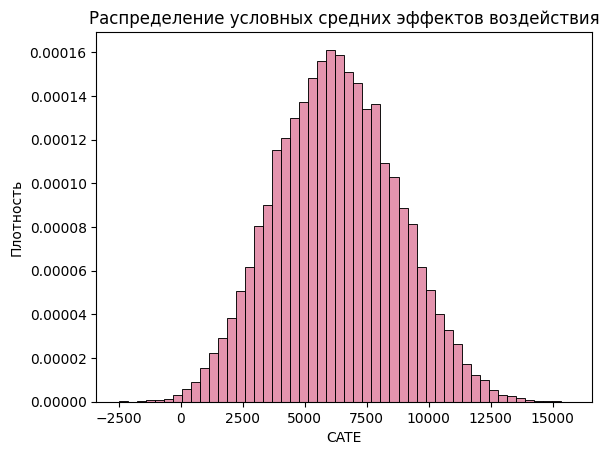
\includegraphics[keepaspectratio,alt={Распределение CATE}]{report_assets/block5_cell_24_output_0.png}}
\caption{Распределение CATE}
\end{figure}

Первые значения \texttt{CATE\_full}: \texttt{7783.72}, \texttt{6017.36},
\texttt{5772.28}, \texttt{939.15}, \texttt{6502.53}, \texttt{5183.60},
\texttt{8234.62}, \texttt{5998.70}, \texttt{6951.41}, \texttt{8082.29}.

    Распределение CATE показывает гетерогенность эффекта: премиум-подписка
приносит разный прирост месячных трат для разных сегментов клиентов.

    \subsection{5.3}\label{section}

\textbf{Задание.} Оцените средний эффект воздействия как разницу в
средних по выборкам тех, кто получил и не получил воздействие. Опишите
недостатки соответствующего подхода с учетом специфики рассматриваемой
вами экономической проблемы.

\textbf{Ответ.}

Наивная оценка опирается на допущение независимости:

\begin{center}
\begin{adjustbox}{max width=\linewidth}
\(\displaystyle E(monthly\_spending1_i \mid premium\_subscription_i = 1) = E(monthly\_spending1_i),\)
\end{adjustbox}
\end{center}
\begin{center}
\begin{adjustbox}{max width=\linewidth}
\(\displaystyle E(monthly\_spending0_i \mid premium\_subscription_i = 0) = E(monthly\_spending0_i).\)
\end{adjustbox}
\end{center}

Тогда средний эффект воздействия оценивается как разница выборочных
средних:

\begin{center}
\begin{adjustbox}{max width=\linewidth}
\(\displaystyle \widehat{ATE}_{naive} = \frac{1}{n_1}\sum\limits_{i: premium\_subscription_i = 1} monthly\_spending_i - \frac{1}{n_0}\sum\limits_{i: premium\_subscription_i = 0} monthly\_spending_i.\)
\end{adjustbox}
\end{center}

В нашей задаче это допущение не выполняется, потому что на решение о
подписке и на траты одновременно влияет ненаблюдаемая
\texttt{online\_preference}.

    \textbf{Наивная оценка ATE}

{\def\LTcaptype{none} % do not increment counter
\begin{longtable}[]{@{}lr@{}}
\toprule\noalign{}
параметр & оценка \\
\midrule\noalign{}
\endhead
\bottomrule\noalign{}
\endlastfoot
ATE oracle & 6292.96 \\
ATE naive & 9883.19 \\
\end{longtable}
}

    Наивная оценка оказывается существенно выше истинного \texttt{ATE}:
примерно \texttt{9883} против \texttt{6293}. Следовательно, простая
разница средних завышает эффект подписки примерно на \texttt{3590}
денежных единиц.

Как и в семинарской логике, это завышение связано с тем, что разница
средних смешивает два эффекта:

\begin{center}
\begin{adjustbox}{max width=\linewidth}
\(\displaystyle E(monthly\_spending_i \mid premium\_subscription_i = 1) - E(monthly\_spending_i \mid premium\_subscription_i = 0) = ATE + \text{selection bias}.\)
\end{adjustbox}
\end{center}

В нашей задаче смещение возникает из-за самоотбора: клиенты с большей
склонностью к онлайн-покупкам чаще оформляют премиум-подписку и
одновременно больше тратят даже без нее. Поэтому наивная разница средних
улавливает не только причинный эффект подписки, но и исходные различия
между группами. Именно из-за этого для корректного анализа нужны методы,
которые хотя бы частично контролируют наблюдаемую неоднородность, а при
наличии эндогенности затем и инструментальный подход.

    \subsection{5.4}\label{section}

\textbf{Задание.} Используя оценки, полученные лучшими из обученных
ранее классификационных и регрессионных моделей, оцените средний эффект
воздействия с помощью: метода наименьших квадратов; условных
математических ожиданий; взвешивания на обратные вероятности; метода,
обладающего двойной устойчивостью; двойного машинного обучения. Сравните
результаты и назовите ключевую предпосылку этих методов. Содержательно
обсудите причины, по которым она может соблюдаться или нарушаться в
вашем случае. Приведите содержательную экономическую интерпретацию
оценки среднего эффекта воздействия.

\textbf{Ответ.}

Подготовим признаки и лучшие модели из разделов 3 и 4. Здесь под лучшими
моделями понимаются лучшие модели из основных методов курса, без
внешнего \texttt{CatBoost} из повышенной сложности блока 4. Это
осознанное ограничение: \texttt{CatBoost} действительно дал чуть меньший
\texttt{RMSE} в блоке 4, но он был добавлен как внешний benchmark
повышенной сложности; для сопоставимости с семинарскими causal-методами
в блоке 5 используем лучшие sklearn-модели из основной линейки. В блоке
5 из предыдущих разделов переносятся архитектуры и гиперпараметры, а
сами nuisance-модели переобучаются на causal controls \texttt{income},
\texttt{age}, \texttt{urban\_area}, \texttt{family\_size} без
инструмента \texttt{free\_trial\_banner}. Поэтому метрики ниже
используются как обоснование выбора класса модели, а не как качество
ровно той же матрицы признаков.

В разделе 3 лучший классификатор из основных методов выбран по
максимальному \texttt{AUC} на тестовой выборке: это градиентный бустинг
(\texttt{AUC\ =\ 0.764}) с параметрами \texttt{n\_estimators\ =\ 100},
\texttt{learning\_rate\ =\ 0.10}, \texttt{max\_depth\ =\ 2}. Этот
критерий подходит для propensity score, потому что нам важна не только
бинарная метка, но и качество ранжирования клиентов по вероятности
подписки.

В разделе 4 лучшая регрессионная модель из основных методов выбрана по
минимальному \texttt{RMSE} на тестовой выборке после тюнинга: это
градиентный бустинг (\texttt{RMSE\ test\ =\ 4710.36}) с параметрами
\texttt{n\_estimators\ =\ 120}, \texttt{learning\_rate\ =\ 0.10},
\texttt{max\_depth\ =\ 3}. \texttt{RMSE} используется как основной
критерий, потому что \texttt{MAPE} менее устойчив из-за малых значений
\texttt{monthly\_spending}.

Основная предпосылка методов этого пункта --- условная независимость
воздействия после учета наблюдаемых признаков:

\begin{center}
\begin{adjustbox}{max width=\linewidth}
\(\displaystyle E(monthly\_spending1_i \mid premium\_subscription_i = 1, X_i) = E(monthly\_spending1_i \mid X_i),\)
\end{adjustbox}
\end{center}
\begin{center}
\begin{adjustbox}{max width=\linewidth}
\(\displaystyle E(monthly\_spending0_i \mid premium\_subscription_i = 0, X_i) = E(monthly\_spending0_i \mid X_i).\)
\end{adjustbox}
\end{center}

Если она выполнена, то различия между клиентами с подпиской и без
подписки можно скорректировать с помощью наблюдаемых признаков
\texttt{X\ =\ (income,\ age,\ urban\_area,\ family\_size)}.

    Эти модели используются как nuisance-модели: регрессия оценивает
условные средние трат, а классификатор оценивает вероятность получения
воздействия.

    Сначала оценим \texttt{ATE} с помощью МНК, отдельно аппроксимируя
месячные траты для клиентов с подпиской и без подписки. Это повторяет
идею из семинара: мы строим две модели условных математических ожиданий,
а затем усредняем разность предсказаний по всей выборке.

При таком подходе

\begin{center}
\begin{adjustbox}{max width=\linewidth}
\(\displaystyle \widehat{ATE}_{LS} = \frac{1}{n}\sum\limits_{i=1}^{n}\left(\widehat{E}(monthly\_spending1_i \mid X_i) - \widehat{E}(monthly\_spending0_i \mid X_i)\right),\)
\end{adjustbox}
\end{center}

а индивидуальная разность прогнозов дает оценку условного эффекта

\begin{center}
\begin{adjustbox}{max width=\linewidth}
\(\displaystyle \widehat{CATE}^{LS}_i = \widehat{E}(monthly\_spending1_i \mid X_i) - \widehat{E}(monthly\_spending0_i \mid X_i).\)
\end{adjustbox}
\end{center}

То есть МНК здесь выступает не только как способ получить средний
эффект, но и как первый, самый простой способ аппроксимировать
гетерогенность воздействия по наблюдаемым признакам.

    \textbf{ATE по МНК}

{\def\LTcaptype{none} % do not increment counter
\begin{longtable}[]{@{}lr@{}}
\toprule\noalign{}
параметр & оценка \\
\midrule\noalign{}
\endhead
\bottomrule\noalign{}
\endlastfoot
ATE oracle & 6292.96 \\
ATE naive & 9883.19 \\
ATE ls & 8034.57 \\
\end{longtable}
}

    Оценка \texttt{ATE\_ls} равна примерно \texttt{8035}, то есть она
заметно ниже наивной оценки, но все еще существенно выше истинного
\texttt{ATE\ =\ 6293}. Это означает, что учет наблюдаемых признаков
действительно снимает часть селекционного смещения, но не устраняет его
полностью.

Причина в том, что линейная спецификация остается достаточно грубой по
сравнению с истинным механизмом генерации данных, а ненаблюдаемая
\texttt{online\_preference} вообще не входит в модель. Поэтому МНК
корректирует различия по \texttt{income}, \texttt{age},
\texttt{urban\_area} и \texttt{family\_size}, но не может удалить
смещение, связанное со скрытой склонностью к онлайн-потреблению.
Содержательно это хороший первый benchmark: он лучше наивной разницы
средних, но еще не решает проблему эндогенности.

    Теперь оценим ATE через условные математические ожидания с помощью
T-learner: одна модель обучается на клиентах без подписки, вторая --- на
клиентах с подпиской.

В терминах семинара это оценка вида

\begin{center}
\begin{adjustbox}{max width=\linewidth}
\(\displaystyle \widehat{CATE}^{T}_i = \widehat{E}(monthly\_spending_i \mid X_i, premium\_subscription_i = 1) - \widehat{E}(monthly\_spending_i \mid X_i, premium\_subscription_i = 0),\)
\end{adjustbox}
\end{center}

а средний эффект воздействия получается усреднением этих условных
эффектов:

\begin{center}
\begin{adjustbox}{max width=\linewidth}
\(\displaystyle \widehat{ATE}^{T} = \frac{1}{n}\sum\limits_{i=1}^{n} \widehat{CATE}^{T}_i.\)
\end{adjustbox}
\end{center}

    \textbf{ATE через условные математические ожидания}

{\def\LTcaptype{none} % do not increment counter
\begin{longtable}[]{@{}lr@{}}
\toprule\noalign{}
параметр & оценка \\
\midrule\noalign{}
\endhead
\bottomrule\noalign{}
\endlastfoot
ATE oracle & 6292.96 \\
ATE naive & 9883.19 \\
ATE ls & 8034.57 \\
ATE conditional means & 7840.64 \\
\end{longtable}
}

    T-learner также дает оценку выше истинного ATE. Метод лучше учитывает
нелинейности, но не решает проблему ненаблюдаемой переменной, влияющей и
на подписку, и на траты.

    Оценим \texttt{ATE} с помощью \texttt{DoubleML} без инструментальной
переменной. Как и в семинаре, здесь используются две nuisance-функции:

\begin{center}
\begin{adjustbox}{max width=\linewidth}
\(\displaystyle g(d, X_i) = E(monthly\_spending_i \mid premium\_subscription_i = d, X_i),\)
\end{adjustbox}
\end{center}

\begin{center}
\begin{adjustbox}{max width=\linewidth}
\(\displaystyle m(X_i) = P(premium\_subscription_i = 1 \mid X_i).\)
\end{adjustbox}
\end{center}

Затем эти оценки подставляются в ортогонализованную moment-функцию. Идея
такого подхода в том, что итоговая оценка становится менее
чувствительной к малым ошибкам в оценивании вспомогательных объектов, а
\texttt{cross-fitting} помогает уменьшить переобучение.

По сравнению с простыми plug-in методами \texttt{DML} особенно полезен
тогда, когда условные средние и propensity score оцениваются гибкими
ML-моделями, а не жесткими линейными спецификациями.

    \textbf{DoubleML без инструмента}

{\def\LTcaptype{none} % do not increment counter
\begin{longtable}[]{@{}lr@{}}
\toprule\noalign{}
показатель & значение \\
\midrule\noalign{}
\endhead
\bottomrule\noalign{}
\endlastfoot
ATE dml standard & 7810.00 \\
std err & 74.435 \\
95\% CI lower & 7664.11 \\
95\% CI upper & 7955.89 \\
\end{longtable}
}

    Оценка \texttt{DoubleML} без инструмента равна примерно \texttt{7810},
то есть она ближе к истинному \texttt{ATE}, чем наивная оценка и МНК, но
все равно остается завышенной. Это хорошо согласуется с экономическим
содержанием задачи.

\texttt{DoubleMLIRM} интерпретируется как оценка \texttt{ATE} только при
допущении условной независимости потенциальных исходов и воздействия
после контроля на \texttt{X}. В нашей генерации это допущение нарушено,
потому что скрытая \texttt{online\_preference} влияет и на вероятность
подписки, и на итоговые траты. Поэтому даже современный
полупараметрический метод с ML nuisance-моделями не может полностью
устранить смещение, если ключевая ненаблюдаемая переменная отсутствует в
данных.

    Далее используем IPW: сначала оценим вероятность подписки по наблюдаемым
признакам, затем построим взвешенный псевдоисход.

IPW-оценка среднего эффекта воздействия имеет вид:

\begin{center}
\begin{adjustbox}{max width=\linewidth}
\(\displaystyle \widehat{ATE}^{IPW} = \frac{1}{n}\sum\limits_{i=1}^{n}\frac{premium\_subscription_i \cdot monthly\_spending_i}{\hat{P}(premium\_subscription_i = 1 \mid X_i)} - \frac{(1 - premium\_subscription_i) \cdot monthly\_spending_i}{1 - \hat{P}(premium\_subscription_i = 1 \mid X_i)}.\)
\end{adjustbox}
\end{center}

Здесь веса корректируют несбалансированность между treated и control
группами по наблюдаемым признакам.

    \textbf{IPW и диагностика propensity score}

{\def\LTcaptype{none} % do not increment counter
\begin{longtable}[]{@{}lr@{}}
\toprule\noalign{}
показатель & оценка \\
\midrule\noalign{}
\endhead
\bottomrule\noalign{}
\endlastfoot
min propensity & 0.012 \\
max propensity & 0.950 \\
ATE IPW & 7816.84 \\
\end{longtable}
}

    Оцененные вероятности не равны 0 или 1, поэтому IPW применим технически.
Содержательно результат также опирается на условную независимость и
поэтому не полностью устраняет эндогенность подписки.

    Теперь рассчитаем \texttt{DR}-оценку. Как и в семинаре, она объединяет
outcome-модели и propensity score, поэтому обладает свойством двойной
устойчивости.

Формально

\begin{center}
\begin{adjustbox}{max width=\linewidth}
\(\displaystyle \widehat{ATE}^{DR} = \frac{1}{n}\sum\limits_{i=1}^{n}\widehat{E}(monthly\_spending_i \mid X_i, T_i = 1) - \widehat{E}(monthly\_spending_i \mid X_i, T_i = 0) + \frac{T_i \cdot (monthly\_spending_i - \widehat{E}(monthly\_spending_i \mid X_i, T_i = 1))}{\hat{P}(T_i = 1 \mid X_i)} - \frac{(1-T_i) \cdot (monthly\_spending_i - \widehat{E}(monthly\_spending_i \mid X_i, T_i = 0))}{1 - \hat{P}(T_i = 1 \mid X_i)}.\)
\end{adjustbox}
\end{center}

Преимущество состоит в том, что при корректной спецификации хотя бы
одной из двух частей, модели исхода или модели вероятности воздействия,
оценка сохраняет состоятельность. Поэтому \texttt{DR} удобно
рассматривать как более надежный benchmark, чем чистый
outcome-regression или чистый \texttt{IPW}.

    \textbf{Сравнение ATE до PSM}

{\def\LTcaptype{none} % do not increment counter
\begin{longtable}[]{@{}lr@{}}
\toprule\noalign{}
метод & оценка \\
\midrule\noalign{}
\endhead
\bottomrule\noalign{}
\endlastfoot
ATE oracle & 6292.96 \\
ATE naive & 9883.19 \\
ATE ls & 8034.57 \\
ATE conditional means & 7840.64 \\
ATE dml standard & 7810.00 \\
ATE IPW & 7816.84 \\
ATE DR & 7819.54 \\
\end{longtable}
}

    Сводная таблица показывает, что все методы на наблюдаемых данных дают
положительный эффект подписки, но практически все они завышают истинный
\texttt{ATE\ =\ 6293}. Наивная оценка максимальна, что соответствует
сильному смещению отбора. После учета наблюдаемых признаков оценки
снижаются: \texttt{ATE\ conditional\ means\ ≈\ 7841},
\texttt{ATE\ dml\ standard\ ≈\ 7810}, \texttt{ATE\ IPW\ ≈\ 7817},
\texttt{ATE\ DR\ ≈\ 7820}.

Наиболее близкими к истинному \texttt{ATE} среди этих методов
оказываются \texttt{T-learner}, \texttt{DML}, \texttt{IPW} и
\texttt{DR}, но даже они остаются выше эталона. Содержательно это
означает, что контроль по наблюдаемым переменным действительно убирает
часть смещения, но скрытая \texttt{online\_preference} не позволяет
полностью восстановить причинный эффект на основе только условия
условной независимости.

Экономическая интерпретация при этом стабильна: премиум-подписка
повышает траты, но если игнорировать ненаблюдаемую селекцию, масштаб
эффекта легко переоценить.

    \textbf{Повышенная сложность. Ответ.} В качестве дополнительного метода
оценки \texttt{ATE} используем \texttt{Propensity\ Score\ Matching}.

Как и в классической постановке из семинарской логики, сначала
оценивается propensity score

\begin{center}
\begin{adjustbox}{max width=\linewidth}
\(\displaystyle p(X_i) = P(premium\_subscription_i = 1 \mid X_i),\)
\end{adjustbox}
\end{center}

после чего treated и control наблюдения сопоставляются по близости этих
вероятностей. Идея \texttt{PSM} состоит в том, что если после
conditioning на \texttt{p(X)} распределения наблюдаемых признаков в
группах становятся близкими, то сравнение исходов внутри matched-пар
лучше приближает причинный эффект, чем сырая разница средних.

В текущем ноутбуке для оценки \texttt{propensity\ score} используется
логистическая регрессия со стандартизацией признаков, а затем
применяется симметричное \texttt{nearest-neighbor\ matching}. Такой
выбор остается достаточно простым, хорошо интерпретируется и
соответствует классическому изложению метода.

    \textbf{PSM: common support и caliper}

\begin{figure}
\centering
\pandocbounded{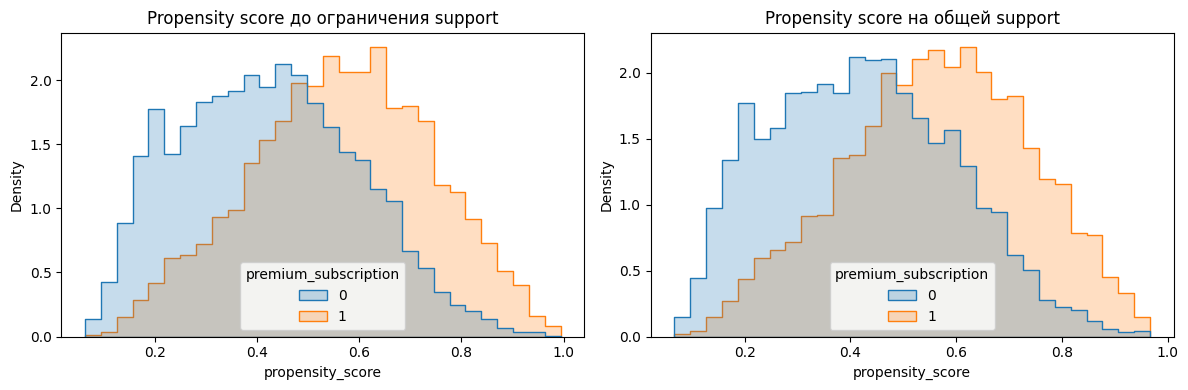
\includegraphics[keepaspectratio,alt={Propensity score и common support}]{report_assets/block5_cell_48_output_0.png}}
\caption{Propensity score и common support}
\end{figure}

{\def\LTcaptype{none} % do not increment counter
\begin{longtable}[]{@{}lr@{}}
\toprule\noalign{}
показатель & оценка \\
\midrule\noalign{}
\endhead
\bottomrule\noalign{}
\endlastfoot
нижняя граница support & 0.067 \\
верхняя граница support & 0.966 \\
доля на общей support & 0.999 \\
caliper по logit propensity & 0.175 \\
\end{longtable}
}

Почти вся выборка находится на общей support, однако нижняя граница
propensity score близка к нулю. Поэтому для методов, основанных на
обратных вероятностях, далее важно контролировать экстремальные веса:
формально нулевых вероятностей нет, но слабый overlap может повышать
дисперсию оценок.

    Для оценки \texttt{ATE} применим симметричное
\texttt{nearest-neighbor\ matching} с возвращением: propensity score
оценивается логистической регрессией, а matching и \texttt{caliper}
считаются в одной шкале \texttt{logit\ propensity\ score}.

Для каждого клиента с подпиской подбирается ближайший клиент без
подписки, а для каждого клиента без подписки --- ближайший клиент с
подпиской. После этого индивидуальные matched-разности усредняются по
общей support. Такой вариант удобен тем, что он ориентирован именно на
оценку среднего эффекта воздействия по всей рабочей выборке, а не только
на \texttt{ATT}.

Идея общей support здесь принципиальна: сравнивать можно только те
наблюдения, для которых в противоположной группе есть достаточно похожие
аналоги по propensity score; само расстояние при matching считается по
\texttt{logit\_ps}.

    \textbf{PSM: matched estimate}

{\def\LTcaptype{none} % do not increment counter
\begin{longtable}[]{@{}lr@{}}
\toprule\noalign{}
показатель & оценка \\
\midrule\noalign{}
\endhead
\bottomrule\noalign{}
\endlastfoot
matched treated & 4914 \\
matched control & 5072 \\
ATE PSM & 8019.06 \\
PSM - true ATE & 1726.10 \\
\textbar PSM - true ATE\textbar{} & 1726.10 \\
\end{longtable}
}

    Проверим баланс контрольных переменных до и после matching с помощью
\texttt{standardized\ mean\ differences}. Здесь \texttt{SMD\ before}
считается не на всей исходной выборке, а на наблюдениях общей support до
matching:

\begin{center}
\begin{adjustbox}{max width=\linewidth}
\(\displaystyle SMD(X_j) = \frac{\bar{X}_{1j} - \bar{X}_{0j}}{\sqrt{\frac{Var(X_{1j}) + Var(X_{0j})}{2}}}.\)
\end{adjustbox}
\end{center}

Именно так, как обсуждается в стандартной теории matching, после
хорошего сопоставления абсолютные значения \texttt{SMD} должны
уменьшаться и становиться близкими к нулю. В наших результатах это и
происходит: по всем контрольным переменным баланс после matching заметно
улучшается.

При этом сама \texttt{ATE\ PSM} оценка остается около \texttt{8019}, то
есть все равно заметно выше истинного \texttt{ATE}. Следовательно,
\texttt{PSM} хорошо выравнивает наблюдаемую часть различий между
группами, но не может убрать смещение, вызванное ненаблюдаемой
\texttt{online\_preference}.

    \textbf{PSM: баланс covariates и итоговая ATE-таблица}

{\def\LTcaptype{none} % do not increment counter
\begin{longtable}[]{@{}lrrrr@{}}
\toprule\noalign{}
переменная & SMD before & SMD after & \textbar SMD before\textbar{} &
\textbar SMD after\textbar{} \\
\midrule\noalign{}
\endhead
\bottomrule\noalign{}
\endlastfoot
income & 0.455 & -0.0090 & 0.455 & 0.0090 \\
age & -0.274 & -0.0070 & 0.274 & 0.0070 \\
urban\_area & 0.458 & 0.017 & 0.458 & 0.017 \\
family\_size & 0.289 & -0.016 & 0.289 & 0.016 \\
\end{longtable}
}

{\def\LTcaptype{none} % do not increment counter
\begin{longtable}[]{@{}lr@{}}
\toprule\noalign{}
метод & оценка \\
\midrule\noalign{}
\endhead
\bottomrule\noalign{}
\endlastfoot
ATE oracle & 6292.96 \\
ATE naive & 9883.19 \\
ATE ls & 8034.57 \\
ATE conditional means & 7840.64 \\
ATE dml standard & 7810.00 \\
ATE IPW & 7816.84 \\
ATE DR & 7819.54 \\
ATE PSM & 8019.06 \\
\end{longtable}
}

    \texttt{Propensity\ Score\ Matching} хорошо подходит здесь как
дополнительный метод оценки \texttt{ATE}, потому что он напрямую решает
задачу сопоставления treated и control клиентов по наблюдаемым
признакам. По сравнению с \texttt{IPW} метод обычно менее чувствителен к
экстремальным весам, а по сравнению с \texttt{OLS} и \texttt{T-learner}
делает акцент именно на сопоставимости групп. Слабая сторона
\texttt{PSM} состоит в возможной потере наблюдений вне общей support и в
том, что метод по-прежнему не устраняет смещение из-за ненаблюдаемой
\texttt{online\_preference}.

В наших данных \texttt{PSM} заметно улучшает баланс наблюдаемых
признаков: абсолютные \texttt{SMD} после matching становятся очень
малыми. Однако сама оценка \texttt{ATE\ PSM} равна примерно
\texttt{8019}, то есть все равно заметно выше истинного
\texttt{ATE\ =\ 6293}. Поэтому содержательный вывод такой: как
дополнительный метод для пункта \texttt{5.4} \texttt{PSM} зашел хорошо,
но полностью проблему эндогенности он не решает.

    \subsection{5.5}\label{section}

\textbf{Задание.} Оцените условные средние эффекты воздействия с
помощью: метода наименьших квадратов; S-learner; T-learner; метода
трансформации классов; X-learner. Сравните результаты и обсудите,
насколько в вашем случае мотивированы применение метода X-learner.
Опишите, как можно было бы использовать полученные вами оценки в бизнесе
или при реализации государственных программ.

\textbf{Ответ.}

Напомним, что условный средний эффект воздействия определяется как

\begin{center}
\begin{adjustbox}{max width=\linewidth}
\(\displaystyle CATE_i = E(monthly\_spending1_i \mid X_i) - E(monthly\_spending0_i \mid X_i).\)
\end{adjustbox}
\end{center}

CATE по МНК и T-learner уже были рассчитаны выше. Теперь оценим CATE с
помощью S-learner: обучим одну модель на признаках и индикаторе
подписки, а затем подставим каждому клиенту оба значения воздействия.

    \texttt{S-learner} использует одну общую модель для обеих групп и
восстанавливает эффект через разность двух counterfactual-прогнозов
одной и той же функции. Это удобно, потому что вся выборка используется
совместно, а сама процедура вычислительно проста.

Однако, как и подчеркивается в семинарской теории, при слабом сигнале
воздействия или при очень разных структурных зависимостях в treated и
control группах такой подход может сглаживать индивидуальные эффекты.
Одна общая модель может слишком сильно усреднять поведение двух режимов
и тем самым недооценивать или переоценивать heterogeneity.

    Оценим CATE методом трансформации классов: модель обучается
прогнозировать IPW-псевдоисход, который является шумной индивидуальной
оценкой эффекта.

В этом подходе сначала строится псевдоисход

\begin{center}
\begin{adjustbox}{max width=\linewidth}
\(\displaystyle monthly\_spending_i^{*} = \frac{premium\_subscription_i \cdot monthly\_spending_i}{\hat{P}(premium\_subscription_i = 1 \mid X_i)} - \frac{(1-premium\_subscription_i) \cdot monthly\_spending_i}{1 - \hat{P}(premium\_subscription_i = 1 \mid X_i)},\)
\end{adjustbox}
\end{center}

а затем оценивается условное математическое ожидание

\begin{center}
\begin{adjustbox}{max width=\linewidth}
\(\displaystyle \widehat{CATE}^{CT}_i = \widehat{E}(monthly\_spending_i^{*} \mid X_i).\)
\end{adjustbox}
\end{center}

    Метод трансформации классов прост в реализации, потому что сводит задачу
оценки \texttt{CATE} к обычной задаче регрессии на псевдоисход. Но цена
этой простоты --- высокая дисперсия.

В наших результатах это видно особенно хорошо: \texttt{CT} дает самый
высокий \texttt{MSE0} среди рассмотренных \texttt{CATE}-методов. Это
означает, что в данной задаче шум в \texttt{IPW}-псевдоисходах слишком
велик, и модель хуже восстанавливает индивидуальную гетерогенность
эффекта, чем \texttt{S-learner}, \texttt{X-learner} и даже
\texttt{T-learner}.

    Оценим CATE с помощью X-learner. Сначала строятся имитированные эффекты
для treated и control групп, затем эти эффекты прогнозируются и
объединяются с весами, связанными с вероятностью подписки.

Для клиентов с подпиской и без подписки строятся две вспомогательные
величины:

\begin{center}
\begin{adjustbox}{max width=\linewidth}
\(\displaystyle D1_i = monthly\_spending_i - \widehat{E}(monthly\_spending0_i \mid X_i), \qquad premium\_subscription_i = 1,\)
\end{adjustbox}
\end{center}
\begin{center}
\begin{adjustbox}{max width=\linewidth}
\(\displaystyle D0_i = \widehat{E}(monthly\_spending1_i \mid X_i) - monthly\_spending_i, \qquad premium\_subscription_i = 0.\)
\end{adjustbox}
\end{center}

После этого оцениваются условные ожидания этих величин и объединяются в
итоговую оценку

\begin{center}
\begin{adjustbox}{max width=\linewidth}
\(\displaystyle \widehat{CATE}^{X}_i = \hat{p}(X_i) \cdot \widehat{E}(D0_i \mid X_i) + (1-\hat{p}(X_i)) \cdot \widehat{E}(D1_i \mid X_i),\)
\end{adjustbox}
\end{center}

где \(\hat{p}(X_i)\) --- оцененная вероятность подписки.

    \texttt{X-learner} особенно мотивирован в нашей задаче по двум причинам,
как и в семинаре. Во-первых, сам эффект подписки гетерогенен. Во-вторых,
treated и control группы различаются по составу, поэтому полезно
отдельно использовать информацию о псевдоэффектах, получаемых внутри
каждой группы.

Именно поэтому \texttt{X-learner} часто работает лучше в задачах, где
есть структурная неоднородность и разная информативность двух
подвыборок. В наших данных этот вывод подтверждается численно: по
\texttt{MSE0} именно \texttt{X-learner} показывает наилучшее качество
восстановления истинного \texttt{CATE}.

    \textbf{Повышенная сложность. Ответ.} В качестве дополнительного метода
повышенной сложности оценим \texttt{CATE} с помощью \texttt{R-learner}.
Идея метода состоит в том, чтобы сначала убрать из
\texttt{monthly\_spending} и \texttt{premium\_subscription} часть,
объясняемую наблюдаемыми признаками, а затем восстанавливать
гетерогенный эффект по остаткам.

Базовое уравнение имеет вид

\begin{center}
\begin{adjustbox}{max width=\linewidth}
\(\displaystyle monthly\_spending_i - m(X_i) = \tau(X_i) \cdot (premium\_subscription_i - e(X_i)) + \varepsilon_i,\)
\end{adjustbox}
\end{center}

где \(m(X_i) = E(monthly\_spending_i \mid X_i)\),
\(e(X_i) = P(premium\_subscription_i = 1 \mid X_i)\), а \(\tau(X_i)\)
--- искомый условный эффект воздействия. Такой подход хорошо подходит
здесь как дополнительный метод \texttt{CATE}, потому что он отдельно
моделирует outcome и propensity score, а затем оценивает именно
гетерогенный эффект.

    \textbf{R-learner: основные результаты}

{\def\LTcaptype{none} % do not increment counter
\begin{longtable}[]{@{}lr@{}}
\toprule\noalign{}
показатель & оценка \\
\midrule\noalign{}
\endhead
\bottomrule\noalign{}
\endlastfoot
share kept after trimming & 1.000 \\
mean R-learner CATE & 7582.08 \\
mean R-learner CATE - true ATE & 1289.12 \\
mean individual bias & 1293.64 \\
\end{longtable}
}

    В \texttt{R-learner} мы используем residualization-подход: сначала
оцениваем \texttt{m(X)} и \texttt{e(X)}, затем переходим к остаткам
исхода и воздействия. Это упрощенная реализация \texttt{R-learner} без
cross-fitting, поэтому возможна зависимость от качества nuisance-моделей
и переобучения.

Фактически оценивается уравнение

\begin{center}
\begin{adjustbox}{max width=\linewidth}
\(\displaystyle monthly\_spending_i - \hat{m}(X_i) \approx \tau(X_i) \cdot (premium\_subscription_i - \hat{e}(X_i)).\)
\end{adjustbox}
\end{center}

Небольшой \texttt{trimming} по наблюдениям с почти нулевым остатком
воздействия нужен для численной устойчивости. Если величина
\(premium\_subscription_i - \hat{e}(X_i)\) слишком мала, то псевдоисход
становится нестабильным и может искусственно увеличивать дисперсию
оценки \texttt{CATE}.

    \textbf{Распределение CATE по R-learner}

\begin{figure}
\centering
\pandocbounded{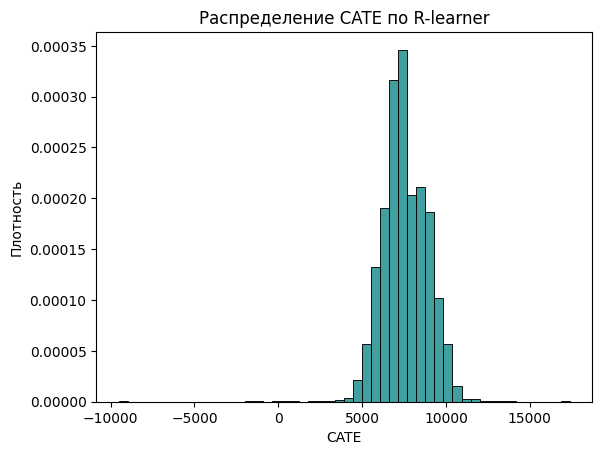
\includegraphics[keepaspectratio,alt={Распределение CATE по R-learner}]{report_assets/block5_cell_66_output_0.png}}
\caption{Распределение CATE по R-learner}
\end{figure}

    \texttt{R-learner} занимает промежуточное место между уже
использованными подходами. По сравнению с \texttt{S-learner} он меньше
зависит от того, насколько одна общая модель умеет различать treatment
heterogeneity. По сравнению с \texttt{T-learner} он эффективнее
использует общую информацию о вероятности подписки и среднем уровне
исхода. По сравнению с методом трансформации классов \texttt{R-learner}
обычно устойчивее, потому что не строится напрямую только на шумном
\texttt{IPW}-псевдоисходе. По сравнению с \texttt{X-learner} его плюс в
явной residualization-логике, а минус в чувствительности к качеству
nuisance-моделей \(m(X)\) и \(e(X)\).

На наших данных \texttt{R-learner} дает средний \texttt{CATE\ ≈\ 7582},
то есть по среднему уровню он ближе к истинному \texttt{ATE}, чем
остальные CATE-методы. По \texttt{RMSE} он почти совпадает с
\texttt{X-learner} и немного лучше \texttt{S-learner}, но по корреляции
с истинным \texttt{CATE} уступает \texttt{X-learner}, \texttt{S-learner}
и МНК. Значит, как дополнительный метод повышенной сложности
\texttt{R-learner} здесь сработал содержательно корректно, но не
является однозначно лучшим по всем критериям индивидуальной
гетерогенности.

    Сравним \texttt{CATE}-оценки с истинными значениями, доступными в
симуляции. Это ключевое преимущество учебной постановки: в реальных
данных истинный \texttt{CATE\_i} недоступен, а здесь мы можем напрямую
измерить качество восстановления гетерогенности.

Поэтому далее удобно смотреть не только на отдельные примеры
предсказаний, но и на интегральные критерии качества по всей выборке.

    Таблица показывает индивидуальные оценки \texttt{CATE} для каждого
метода. Для качества сравнения, как и в семинаре, удобно использовать
среднеквадратичную ошибку относительно истинного \texttt{CATE}:

\begin{center}
\begin{adjustbox}{max width=\linewidth}
\(\displaystyle MSE_0 = \frac{1}{n}\sum\limits_{i=1}^{n}(CATE_i - \widehat{CATE}_i)^2.\)
\end{adjustbox}
\end{center}

Кроме того, полезно смотреть на

\begin{center}
\begin{adjustbox}{max width=\linewidth}
\(\displaystyle RMSE = \sqrt{MSE_0}, \qquad MAE = \frac{1}{n}\sum\limits_{i=1}^{n}|CATE_i - \widehat{CATE}_i|,\)
\end{adjustbox}
\end{center}

а также на среднее значение предсказанного \texttt{CATE}, его смещение
относительно истинного среднего эффекта и корреляцию с истинным
\texttt{CATE}. Такой набор метрик позволяет разделить два вопроса:
насколько хорошо метод восстанавливает средний уровень эффекта и
насколько хорошо он ранжирует клиентов по индивидуальной гетерогенности.

    \textbf{Качество CATE-оценок относительно oracle-CATE}

{\def\LTcaptype{none} % do not increment counter
\begin{longtable}[]{@{}lrrrrr@{}}
\toprule\noalign{}
метод & mean CATE & bias mean & RMSE & MAE & corr with true CATE \\
\midrule\noalign{}
\endhead
\bottomrule\noalign{}
\endlastfoot
LS & 8034.57 & 1741.61 & 2588.92 & 2119.93 & 0.617 \\
T-learner & 7840.64 & 1547.68 & 2503.46 & 2023.76 & 0.588 \\
S-learner & 7785.13 & 1492.17 & 2450.86 & 1989.37 & 0.604 \\
CT & 7816.84 & 1523.88 & 3691.49 & 2529.43 & 0.410 \\
X-learner & 7751.17 & 1458.21 & 2429.07 & 1966.27 & 0.605 \\
R-learner & 7582.08 & 1289.12 & 2431.15 & 1943.29 & 0.530 \\
\end{longtable}
}

    По нашим метрикам лучше всего гетерогенность эффекта по \texttt{MSE0}
восстанавливает \texttt{X-learner}: у него минимальный
\texttt{MSE0\ ≈\ 5.9\ \textbackslash{}cdot\ 10\^{}6} и наименьший
\texttt{RMSE} среди рассматриваемых методов. \texttt{R-learner} идет
практически рядом по \texttt{RMSE} и имеет меньший \texttt{MAE}, а
\texttt{S-learner} также показывает сильный результат. Метод
трансформации классов заметно хуже по \texttt{MSE0} из-за высокой
дисперсии IPW-псевдоисходов.

Содержательно это означает, что для задач, где важна точность
индивидуальной величины эффекта, \texttt{X-learner} в этой симуляции
выглядит наиболее убедительно по основной MSE-метрике. Если же акцент
делать именно на ранжировке клиентов, нужно также смотреть на корреляцию
с истинным \texttt{CATE}: по ней лучшим оказывается МНК, а
\texttt{X-learner} и \texttt{S-learner} идут близко. Такие оценки можно
использовать, например, для показа премиум-офера тем клиентам, у которых
предсказанный прирост трат максимален, но решение лучше проверять по
нескольким метрикам одновременно.

    Дополнительно сравним CATE-оценки с IPW-псевдоисходами. Этот критерий
более шумный, но показывает, насколько методы близки к
псевдоиндивидуальным эффектам, построенным только на наблюдаемых данных.

Соответствующий критерий имеет вид:

\begin{center}
\begin{adjustbox}{max width=\linewidth}
\(\displaystyle MSE_1 = \frac{1}{n}\sum\limits_{i=1}^{n}(monthly\_spending_i^{*} - \widehat{CATE}_i)^2.\)
\end{adjustbox}
\end{center}

    \textbf{MSE1 по IPW-псевдоисходам}

{\def\LTcaptype{none} % do not increment counter
\begin{longtable}[]{@{}lr@{}}
\toprule\noalign{}
метод & MSE1 \\
\midrule\noalign{}
\endhead
\bottomrule\noalign{}
\endlastfoot
LS & 508965200.00 \\
T-learner & 507271700.00 \\
S-learner & 509209600.00 \\
CT & 478352600.00 \\
X-learner & 508492900.00 \\
R-learner & 507514900.00 \\
\end{longtable}
}

    Значения \texttt{MSE1} по псевдоисходам существенно больше, потому что
сами \texttt{IPW}-псевдоисходы имеют высокую дисперсию. Поэтому, как и в
семинаре, основной содержательный критерий здесь --- это сравнение с
истинным \texttt{CATE}, а не только с шумной proxy-целью.

В нашем случае по \texttt{MSE1} минимальное значение получается у метода
трансформации классов, потому что он напрямую обучается на том же
IPW-псевдоисходе. Но это не означает, что он лучше восстанавливает
истинный \texttt{CATE}: по \texttt{MSE0} относительно симуляционного
oracle-CATE метод \texttt{CT} оказывается худшим. Поэтому главный вывод
делаем по \texttt{MSE0}, а \texttt{MSE1} используем только как
дополнительную диагностику близости к шумной proxy-цели.

    \subsection{5.6}\label{section}

\textbf{Задание.} Оцените локальный средний эффект воздействия с
помощью: двойного машинного обучения без инструментальной переменной;
двойного машинного обучения с инструментальной переменной. Сопоставьте
результаты и объясните, в чем в вашем случае будет заключаться различие
между средним эффектом воздействия и локальным средним эффектом
воздействия. Приведите содержательную экономическую интерпретацию оценки
локального среднего эффекта воздействия.

\textbf{Ответ.}

Как и в семинаре, здесь важно отделить проблему \texttt{ATE} от проблемы
\texttt{LATE}. При наличии эндогенности без инструмента можно пытаться
оценивать \texttt{ATE} только при очень сильной предпосылке условной
независимости. Если же эта предпосылка нарушена, то инструментальный
подход позволяет идентифицировать не средний эффект для всех клиентов, а
локальный средний эффект для соблюдателей.

Сначала построим \texttt{DML} без инструмента. Технически это
\texttt{DoubleMLIRM}, поэтому он оценивает \texttt{ATE} при условной
независимости, а не полноценный \texttt{LATE}. Без инструментальной
переменной локальный эффект для соблюдателей в том же смысле, что и
IV-\texttt{LATE}, не идентифицируется. Поэтому этот результат
используется ниже как \texttt{ATE/DML}-бенчмарк без инструмента: он
показывает, что дает causal ML при игнорировании инструментальной
структуры, но не является самостоятельной оценкой \texttt{LATE}.

    Перед DML-оценками зафиксируем важную техническую деталь сравнения.
Истинные \texttt{ATE} и \texttt{LATE} выше рассчитаны на полной выборке
из 30000 наблюдений, а DML-оценки ниже строятся на рабочей подвыборке из
10000 наблюдений. Поэтому в таблицах дальше full-sample эффекты остаются
главным эталоном DGP, но для контроля также выводим oracle-эффекты на
самой рабочей подвыборке.

    \textbf{Oracle-эффекты на полной выборке и рабочей подвыборке}

{\def\LTcaptype{none} % do not increment counter
\begin{longtable}[]{@{}lrr@{}}
\toprule\noalign{}
параметр & полная выборка 30000 & рабочая подвыборка 10000 \\
\midrule\noalign{}
\endhead
\bottomrule\noalign{}
\endlastfoot
ATE oracle & 6292.96 & 6324.95 \\
LATE oracle & 6280.32 & 6328.99 \\
ATET oracle & 7274.64 & 7285.16 \\
\end{longtable}
}

    \textbf{DML без инструмента в 5.6}

{\def\LTcaptype{none} % do not increment counter
\begin{longtable}[]{@{}lr@{}}
\toprule\noalign{}
показатель & значение \\
\midrule\noalign{}
\endhead
\bottomrule\noalign{}
\endlastfoot
ATE/DML no IV benchmark & 7810.00 \\
std err & 74.435 \\
95\% CI lower & 7664.11 \\
95\% CI upper & 7955.89 \\
\end{longtable}
}

    Оценка без инструмента показывает, что будет получено, если игнорировать
инструментальную структуру и опираться только на наблюдаемые признаки. В
нашем случае это дает число \texttt{≈\ 7810}. Его нельзя
интерпретировать как \texttt{LATE}: это бенчмарк для среднего эффекта
при условной независимости. Однако сравнение с oracle-\texttt{LATE}
полезно диагностически: результат заметно выше как full-sample oracle
\texttt{LATE\ =\ 6280}, так и sample oracle \texttt{LATE\ ≈\ 6329}.

Следовательно, если не учитывать эндогенность подписки и не использовать
инструмент, оценка эффекта оказывается завышенной относительно
локального эффекта для соблюдателей. Это ровно та проблема, ради которой
в следующем шаге и нужен \texttt{IV-DML}.

    \textbf{Ответ.} Теперь используем \texttt{DoubleMLIIVM}, где
\texttt{free\_trial\_banner} выступает инструментом для
премиум-подписки. Эта модель оценивает \texttt{LATE} для соблюдателей.

В инструментальном подходе \texttt{DoubleMLIIVM} используются три
nuisance-объекта:

\begin{center}
\begin{adjustbox}{max width=\linewidth}
\(\displaystyle g(Z_i, X_i) = E(monthly\_spending_i \mid X_i, free\_trial\_banner_i = Z_i),\)
\end{adjustbox}
\end{center}
\begin{center}
\begin{adjustbox}{max width=\linewidth}
\(\displaystyle m(X_i) = P(free\_trial\_banner_i = 1 \mid X_i),\)
\end{adjustbox}
\end{center}
\begin{center}
\begin{adjustbox}{max width=\linewidth}
\(\displaystyle r(Z_i, X_i) = P(premium\_subscription_i = 1 \mid X_i, free\_trial\_banner_i = Z_i).\)
\end{adjustbox}
\end{center}

При выполнении условий релевантности, экзогенности и монотонности
инструмента \texttt{DoubleMLIIVM} оценивает именно локальный средний
эффект воздействия. Иными словами, он отвечает на вопрос: каков эффект
подписки для тех клиентов, чье решение о подписке действительно меняется
из-за баннера.

    Перед оценкой \texttt{IV-DML} проверим first stage и состав типов
клиентов. Баннер должен заметно менять вероятность подписки, а
соблюдатели должны иметь ненулевую долю; это поддерживает релевантность
инструмента и содержательную интерпретацию \texttt{LATE}. Доли типов
клиентов (\texttt{Complier}, \texttt{Always\ taker},
\texttt{Never\ taker}) являются oracle-диагностикой из симуляционной
DGP: в реальных данных они напрямую не наблюдаются. Observed first-stage
difference может не совпадать с oracle-долей compliers, потому что
сравнение \texttt{P(D=1\textbar{}Z=1)-P(D=1\textbar{}Z=0)} считается по
фактически получившим и не получившим баннер на конечной подвыборке, где
состав групп по \texttt{X} может отличаться.

    \textbf{First-stage и oracle-типы клиентов}

{\def\LTcaptype{none} % do not increment counter
\begin{longtable}[]{@{}lr@{}}
\toprule\noalign{}
показатель & оценка \\
\midrule\noalign{}
\endhead
\bottomrule\noalign{}
\endlastfoot
P(D=1 \textbar{} Z=0) & 0.411 \\
P(D=1 \textbar{} Z=1) & 0.648 \\
first-stage difference & 0.237 \\
share Complier & 0.162 \\
share Always Taker & 0.438 \\
share Never Taker & 0.400 \\
\end{longtable}
}

    \textbf{IV-DML}

{\def\LTcaptype{none} % do not increment counter
\begin{longtable}[]{@{}lr@{}}
\toprule\noalign{}
показатель & значение \\
\midrule\noalign{}
\endhead
\bottomrule\noalign{}
\endlastfoot
LATE dml IV & 6250.16 \\
std err & 572.89 \\
95\% CI lower & 5127.31 \\
95\% CI upper & 7373.02 \\
\end{longtable}
}

    \texttt{IV-DML} оценивает эффект не для всех клиентов, а для
соблюдателей, то есть для той подгруппы, чье решение о подписке
изменяется под воздействием баннера. В наших данных оценка
\texttt{LATE\ dml\ IV} равна примерно \texttt{6250}. По сравнению с
full-sample oracle \texttt{LATE\ =\ 6280} абсолютное отклонение
составляет около \texttt{30}; по сравнению с sample oracle
\texttt{LATE\ ≈\ 6329} отклонение составляет около \texttt{79}.

Оба сравнения намного лучше бенчмарка без инструмента (\texttt{≈\ 1530}
относительно full-sample \texttt{LATE} и \texttt{≈\ 1481} относительно
sample \texttt{LATE}). Значит, именно введение инструмента радикально
улучшает качество оценки локального эффекта. Экономически это означает,
что баннер позволяет выделить клиентов, для которых подписка
действительно является маржинальным решением, и именно для них эффект
подписки можно оценить особенно содержательно.

    \textbf{Повышенная сложность. Ответ.} Поскольку \texttt{Rscript} и пакет
\texttt{switchSelection} в текущей среде недоступны, оценим
параметрический benchmark без R: two-step endogenous switching model в
Python. Это не полноценная реализация \texttt{switchSelection}/FIML и
ниже не оцениваются стандартные ошибки switching-модели, поэтому
результат используется именно как параметрическая точка сравнения.

На первом шаге оценивается параметрическое selection equation через
probit:

\begin{center}
\begin{adjustbox}{max width=\linewidth}
\(\displaystyle premium\_subscription_i^{*} = \alpha_0 + \alpha_1 free\_trial\_banner_i + X_i'\alpha + u_i, \qquad premium\_subscription_i = 1[premium\_subscription_i^{*} > 0].\)
\end{adjustbox}
\end{center}

На втором шаге отдельно для клиентов с подпиской и без подписки
оцениваются outcome-equations с поправкой Хекмана через inverse Mills
ratio:

\begin{center}
\begin{adjustbox}{max width=\linewidth}
\(\displaystyle monthly\_spending_i = X_i'\beta_1 + \rho_1\sigma_1\lambda_1(X_i,Z_i) + \varepsilon_{1i}, \qquad D_i=1,\)
\end{adjustbox}
\end{center}

\begin{center}
\begin{adjustbox}{max width=\linewidth}
\(\displaystyle monthly\_spending_i = X_i'\beta_0 + \rho_0\sigma_0\lambda_0(X_i,Z_i) + \varepsilon_{0i}, \qquad D_i=0.\)
\end{adjustbox}
\end{center}

Это параметрический подход: и модель выбора режима, и модели исходов
задаются явной функциональной формой. По сравнению с \texttt{IV-DML} он
лучше интерпретируется, но сильнее зависит от корректности
probit-спецификации и линейных outcome-equations.

    \textbf{Параметрический switching benchmark}

{\def\LTcaptype{none} % do not increment counter
\begin{longtable}[]{@{}lr@{}}
\toprule\noalign{}
показатель & оценка \\
\midrule\noalign{}
\endhead
\bottomrule\noalign{}
\endlastfoot
share negative raw complier weights & 0.0000 \\
share clipped or near-zero weights & 0.0000 \\
mean raw complier weight & 0.160 \\
mean clipped complier weight & 0.160 \\
sum clipped complier weights & 1601.94 \\
LATE parametric switching & 8027.34 \\
\textbar parametric switching - true LATE\textbar{} & 1747.02 \\
\end{longtable}
}

    По параметрической switching-модели получаем предсказанные потенциальные
исходы \(\widehat{monthly\_spending1}_i\) и
\(\widehat{monthly\_spending0}_i\), а затем индивидуальный
параметрический эффект

\begin{center}
\begin{adjustbox}{max width=\linewidth}
\(\displaystyle \widehat{\tau}_i = \widehat{monthly\_spending1}_i - \widehat{monthly\_spending0}_i.\)
\end{adjustbox}
\end{center}

Чтобы приблизиться именно к локальному эффекту для соблюдателей,
используем параметрические complier weights:

\begin{center}
\begin{adjustbox}{max width=\linewidth}
\(\displaystyle \widehat{c}_i = \widehat{P}(premium\_subscription_i = 1 \mid free\_trial\_banner_i = 1, X_i) - \widehat{P}(premium\_subscription_i = 1 \mid free\_trial\_banner_i = 0, X_i).\)
\end{adjustbox}
\end{center}

Тогда итоговая параметрическая оценка имеет вид

\begin{center}
\begin{adjustbox}{max width=\linewidth}
\(\displaystyle \widehat{LATE}^{param} = \frac{\sum_i \widehat{c}_i \widehat{\tau}_i}{\sum_i \widehat{c}_i}.\)
\end{adjustbox}
\end{center}

Если из-за численных ошибок некоторые веса оказываются отрицательными,
мы клиппируем их к нулю. Такая процедура делает интерпретацию весов как
вероятностной меры принадлежности к соблюдателям более устойчивой.

    \textbf{Сравнение LATE-оценок}

{\def\LTcaptype{none} % do not increment counter
\begin{longtable}[]{@{}lrr@{}}
\toprule\noalign{}
метод & оценка & \textbar estimate - true LATE\textbar{} \\
\midrule\noalign{}
\endhead
\bottomrule\noalign{}
\endlastfoot
ATE & 6292.96 & 12.641 \\
LATE oracle & 6280.32 & 0.0000 \\
ATE/DML no IV benchmark & 7810.00 & 1529.68 \\
LATE dml IV & 6250.16 & 30.159 \\
LATE parametric switching & 8027.34 & 1747.02 \\
\end{longtable}
}

    \texttt{ATE} относится ко всем клиентам, а \texttt{LATE} --- только к
соблюдателям. В данном исследовании \texttt{LATE} показывает эффект
премиум-подписки для клиентов, которых можно подтолкнуть к подписке
показом баннера. Поэтому строка \texttt{ATE/DML\ no\ IV\ benchmark} в
таблице выше не является оценкой \texttt{LATE}; она оставлена только как
сравнение с подходом, который не использует инструмент и опирается на
условную независимость по наблюдаемым признакам.

Параметрический switching benchmark дает оценку того же локального
эффекта через жесткую функциональную форму: probit для выбора подписки и
две линейные outcome-модели с поправкой на selection. В отличие от
\texttt{IV-DML}, этот подход менее гибкий и чувствителен к спецификации,
зато его легче интерпретировать как явную структурную модель выбора
режима и исходов. Поскольку это ручная two-step-реализация без
стандартных ошибок и без полноценного \texttt{switchSelection},
результат следует использовать только как иллюстративный параметрический
benchmark, а не как надежную финальную оценку. Большое отклонение от
oracle \texttt{LATE} показывает, что в этой DGP линейная
switching-спецификация недостаточно хорошо приближает истинный механизм.

    \subsection{5.7}\label{section}

\textbf{Задание.} Оцените средние эффекты воздействия и локальные
средние эффекты воздействия используя худшие из обученных
классификационных и регрессионных моделей. Сопоставьте результаты с
теми, что были получены с помощью лучших моделей. Сдеайте вывод об
устойчивости результатов к качеству используемых методов машинного
обучения.

\textbf{Ответ.}

В этом пункте, как и в семинаре, сохраняются те же формулы для
\texttt{T-learner}, \texttt{IPW}, \texttt{DR}, \texttt{DML} и
\texttt{IV-DML}, но nuisance-модели заменяются худшими по качеству из
предыдущих разделов.

В разделе 3 худший классификатор из основных методов выбран по
минимальному \texttt{AUC} на тестовой выборке: это логистическая
регрессия (\texttt{AUC\ =\ 0.729}) с параметрами после тюнинга по
accuracy \texttt{C\ =\ 0.01},
\texttt{penalty\ =\ \textquotesingle{}l2\textquotesingle{}}. В разделе 4
худшая регрессионная модель из основных методов выбрана по максимальному
\texttt{RMSE} на тестовой выборке после тюнинга: это МНК
(\texttt{RMSE\ test\ =\ 4983.14}), реализованный как
\texttt{LinearRegression} без дополнительных гиперпараметров. Как и в
пункте 5.4, в блоке 5 эти модели переобучаются на causal controls без
\texttt{free\_trial\_banner}.

Такая замена позволяет проверить, насколько чувствительны оценки
\texttt{ATE} и \texttt{LATE} к ошибкам прогнозирования условных средних
и вероятностей. Если метод устойчив, то замена лучших моделей на худшие
не должна полностью менять качественный вывод. Если же оценка резко
меняется, это означает сильную зависимость итогового causal-вывода от
качества вспомогательных ML-моделей.

    Повторим T-learner, IPW, DR, DML и IV-DML с худшими nuisance-моделями.
Для IPW/DR отдельно проверяем диапазон propensity score: если
вероятность близка к 0 или 1, веса становятся большими и оценки могут
быть нестабильными.

    \textbf{Худшая propensity-модель: диапазон вероятностей}

{\def\LTcaptype{none} % do not increment counter
\begin{longtable}[]{@{}lr@{}}
\toprule\noalign{}
показатель & оценка \\
\midrule\noalign{}
\endhead
\bottomrule\noalign{}
\endlastfoot
worst min prob & 0.073 \\
worst max prob & 0.992 \\
\end{longtable}
}

    Для DML-оценок отдельно создадим объекты \texttt{DoubleMLData} и
применим худшие модели как nuisance-оценки.

    Сопоставим оценки, полученные лучшими и худшими моделями. Это позволяет
отделить два уровня неопределенности: собственно эконометрическую
идентификацию и качество статистического приближения nuisance-объектов.

В наших результатах \texttt{ATE}-оценки при переходе к худшим моделям в
целом сдвигаются вверх, а инструментальная \texttt{LATE\ DML\ IV}
меняется особенно заметно: примерно с \texttt{6250} до \texttt{8450}.
Следовательно, в этой симуляции \texttt{IV-DML} чувствителен к качеству
вспомогательных моделей, потому что в нем одновременно участвуют
outcome-model, treatment-model и instrument-model. Этот вывод относится
именно к реализации с выбранными nuisance-моделями и не отменяет того,
что инструментальная идентификация остается ключевой для работы с
эндогенностью.

    \textbf{Устойчивость к качеству nuisance-моделей}

{\def\LTcaptype{none} % do not increment counter
\begin{longtable}[]{@{}lrr@{}}
\toprule\noalign{}
метод & лучшие модели & худшие модели \\
\midrule\noalign{}
\endhead
\bottomrule\noalign{}
\endlastfoot
ATE ls & 8034.57 & 8034.57 \\
ATE conditional means & 7840.64 & 8034.57 \\
ATE IPW & 7816.84 & 7914.96 \\
ATE DR & 7819.54 & 8065.18 \\
ATE DML & 7810.00 & 8064.23 \\
LATE DML IV & 6250.16 & 8450.27 \\
\end{longtable}
}

    Оценки ATE заметно меняются при переходе к худшим nuisance-моделям, что
говорит о чувствительности результатов к качеству прогнозных моделей.
Строка \texttt{ATE\ ls} не меняется, потому что худшая регрессионная
модель и есть линейная регрессия/МНК, то есть тот же estimator, который
используется в LS-бенчмарке. У худшего propensity максимальная
вероятность близка к 1 (\texttt{0.992}), поэтому IPW/DR с худшими
моделями потенциально менее устойчивы из-за больших обратных весов. Для
LATE через IV-DML различие также может быть существенным, потому что
инструментальная модель требует одновременно хороших моделей исхода,
воздействия и инструмента.

    \subsection{5.8}\label{section}

\textbf{Задание.} Резюмируйте ключевые выводы проведенного в данном
разделе анализа.

\textbf{Ответ.}

Соберем итоговые таблицы раздела, а затем содержательно интерпретируем
их с точки зрения \texttt{ATE}, \texttt{CATE}, \texttt{LATE} и
устойчивости методов.

    \textbf{Итоговые таблицы блока 5}

\textbf{ATE}

{\def\LTcaptype{none} % do not increment counter
\begin{longtable}[]{@{}lr@{}}
\toprule\noalign{}
метод & оценка \\
\midrule\noalign{}
\endhead
\bottomrule\noalign{}
\endlastfoot
ATE oracle & 6292.96 \\
ATE naive & 9883.19 \\
ATE ls & 8034.57 \\
ATE conditional means & 7840.64 \\
ATE dml standard & 7810.00 \\
ATE IPW & 7816.84 \\
ATE DR & 7819.54 \\
ATE PSM & 8019.06 \\
\end{longtable}
}

\textbf{CATE MSE0}

{\def\LTcaptype{none} % do not increment counter
\begin{longtable}[]{@{}lr@{}}
\toprule\noalign{}
метод & MSE0 \\
\midrule\noalign{}
\endhead
\bottomrule\noalign{}
\endlastfoot
LS & 6702512.00 \\
T-learner & 6267289.00 \\
S-learner & 6006731.00 \\
CT & 13627120.00 \\
X-learner & 5900400.00 \\
R-learner & 5910478.00 \\
\end{longtable}
}

\textbf{LATE}

{\def\LTcaptype{none} % do not increment counter
\begin{longtable}[]{@{}lrr@{}}
\toprule\noalign{}
метод & оценка & \textbar estimate - true LATE\textbar{} \\
\midrule\noalign{}
\endhead
\bottomrule\noalign{}
\endlastfoot
ATE & 6292.96 & 12.641 \\
LATE oracle & 6280.32 & 0.0000 \\
ATE/DML no IV benchmark & 7810.00 & 1529.68 \\
LATE dml IV & 6250.16 & 30.159 \\
LATE parametric switching & 8027.34 & 1747.02 \\
\end{longtable}
}

    Проведенный анализ дает несколько важных выводов.

Во-первых, премиум-подписка оказывает положительный причинный эффект на
месячные траты клиентов. Истинный \texttt{ATE} в симуляции на полной
объединенной выборке равен примерно \texttt{6293}, а истинный
\texttt{LATE} --- \texttt{6280}, так что для соблюдателей эффект близок
к среднему эффекту по выборке.

Во-вторых, наивная оценка сильно завышает эффект (\texttt{9883} против
\texttt{6293}) из-за самоотбора. Это подтверждает, что простое сравнение
клиентов с подпиской и без подписки неприменимо, когда существует
ненаблюдаемая переменная, одновременно влияющая и на treatment, и на
outcome.

В-третьих, методы из пункта \texttt{5.4}, основанные на наблюдаемых
признаках, действительно сокращают смещение, но не устраняют его
полностью. Оценки остаются выше эталона, поскольку предпосылка условной
независимости нарушается скрытой \texttt{online\_preference}.

В-четвертых, для оценки гетерогенности эффекта лучшим методом по
\texttt{MSE0} оказывается \texttt{X-learner}; \texttt{R-learner} идет
почти наравне по \texttt{RMSE} и имеет наименьшее смещение среднего
эффекта. При этом для задачи ранжировки важно помнить, что по корреляции
с истинным \texttt{CATE} лучшим оказывается МНК, поэтому таргетирование
лучше оценивать не по одной метрике. Метод трансформации классов
работает хуже по \texttt{MSE0} из-за высокой дисперсии псевдоисходов,
хотя по \texttt{MSE1} он ближе всего к собственному IPW-псевдоисходу.

В-пятых, при наличии эндогенности принципиально важен инструментальный
подход. Бенчмарк \texttt{DML} без инструмента не является оценкой
\texttt{LATE}, потому что без инструмента локальный эффект для
соблюдателей не идентифицируется в том же смысле. Он заметно расходится
с true \texttt{LATE}, тогда как \texttt{IV-DML} дает оценку гораздо
ближе к локальному эффекту для соблюдателей. Параметрический switching
benchmark дает дополнительную точку сравнения, но заметно сильнее
ошибается из-за жестких функциональных предпосылок.

Наконец, проверка устойчивости показывает, что качество nuisance-моделей
действительно важно. При переходе к худшим моделям меняются и
\texttt{ATE}, и особенно \texttt{LATE} через \texttt{IV-DML}. В этом
блоке лучшие/худшие модели трактуются как модели из основной
sklearn-линейки и переобучаются на causal controls без
\texttt{free\_trial\_banner}; внешний \texttt{CatBoost} из повышенной
сложности блока 4 не используется как nuisance-модель ради
сопоставимости с семинарскими методами. Параметрический switching
benchmark также не является полноценным \texttt{switchSelection},
поэтому используется только как иллюстративное сравнение с
\texttt{IV-DML}. Поэтому общий практический вывод такой: causal-методы
машинного обучения полезны и информативны, но их результат нужно
интерпретировать вместе с предпосылками идентификации, качеством
вспомогательных прогнозных моделей и ограничениями выбранной
спецификации.

    \subsection{5.9}\label{section}

\textbf{Задание.} В случае необходимости проведите дополнительный
анализ.

\textbf{Ответ.}

Дополнительный анализ в данном разделе не требуется. Основные оценки
\texttt{ATE}, \texttt{CATE} и \texttt{LATE}, а также проверка
устойчивости к качеству моделей уже проведены. Отдельно была добавлена
повышенная сложность с \texttt{PSM}, \texttt{R-learner} и
параметрическим switching benchmark, поэтому содержательно раздел
покрывает как базовые, так и расширенные подходы к оцениванию эффектов
воздействия.


    % Add a bibliography block to the postdoc
    
    
    
\end{document}
